\RequirePackage{pdfmanagement-testphase}
\DeclareDocumentMetadata {lang=en-US}

% xmp metadata for pdf
% Originally used \usepackage[a-2a]{pdfx}
% \usepackage{hyperxmp} replaced it
% \RequirePackage{pdfmanagement-testphase} replaced it
% \PassOptionsToPackage{enable-debug,check-declarations}{expl3} broke with version 0.9 of tagpdf
% \ExplSyntaxOn no need for these 3 lines because metadata can handle it
% \pdfmanagement_add:nnn{Catalog}{Lang}{(enUS)} enUS is wrong, should be en-US
% \ExplSyntaxOff

\documentclass[11pt,
  english,
  a4paper,
]{article}
\usepackage{sa4ss}
\usepackage{amsmath,amssymb,array}
\usepackage{booktabs}

% From tagged-template.latex
\usepackage{lmodern}
\usepackage{ifxetex,ifluatex}
\ifnum 0\ifxetex 1\fi\ifluatex 1\fi=0 % if pdftex
  \usepackage[T1]{fontenc}
  \usepackage[utf8]{inputenc}
  \usepackage{textcomp} % provide euro and other symbols
\else % if luatex or xetex
  \usepackage{unicode-math}
  \defaultfontfeatures{Scale=MatchLowercase}
  \defaultfontfeatures[\rmfamily]{Ligatures=TeX,Scale=1}
\fi

% Use upquote if available, for straight quotes in verbatim environments
\IfFileExists{upquote.sty}{\usepackage{upquote}}{}
\IfFileExists{microtype.sty}{% use microtype if available
  \usepackage[]{microtype}
  \UseMicrotypeSet[protrusion]{basicmath} % disable protrusion for tt fonts
}{}
\makeatletter
\@ifundefined{KOMAClassName}{% if non-KOMA class
  \IfFileExists{parskip.sty}{%
    \usepackage{parskip}
  }{% else
    \setlength{\parindent}{0pt}
    \setlength{\parskip}{6pt plus 2pt minus 1pt}}
}{% if KOMA class
  \KOMAoptions{parskip=half}}
\makeatother
\usepackage{xcolor}
\IfFileExists{xurl.sty}{\usepackage{xurl}}{} % add URL line breaks if available
\hypersetup{
  pdftitle={The status of copper rockfish (Sebastes caurinus) in U.S. waters off the coast of Oregon in 2021 using catch and length data},
  pdflang={en},
  hidelinks,
  pdfcreator={LaTeX via pandoc}}
\urlstyle{same} % disable monospaced font for URLs
\usepackage{longtable}
% Correct order of tables after \paragraph or \subparagraph
\usepackage{etoolbox}
\makeatletter
\patchcmd\longtable{\par}{\if@noskipsec\mbox{}\fi\par}{}{}
\makeatother
% Allow footnotes in longtable head/foot
\IfFileExists{footnotehyper.sty}{\usepackage{footnotehyper}}{\usepackage{footnote}}
\makesavenoteenv{longtable}
\usepackage{graphicx}
\makeatletter
\def\maxwidth{\ifdim\Gin@nat@width>\linewidth\linewidth\else\Gin@nat@width\fi}
\def\maxheight{\ifdim\Gin@nat@height>\textheight\textheight\else\Gin@nat@height\fi}
\makeatother
% Scale images if necessary, so that they will not overflow the page
% margins by default, and it is still possible to overwrite the defaults
% using explicit options in \includegraphics[width, height, ...]{}
\setkeys{Gin}{width=\maxwidth,height=\maxheight,keepaspectratio}
% Set default figure placement to htbp
\makeatletter
\def\fps@figure{htbp}
\makeatother
\setlength{\emergencystretch}{3em} % prevent overfull lines
\providecommand{\tightlist}{%
  \setlength{\itemsep}{0pt}\setlength{\parskip}{0pt}}
\setcounter{secnumdepth}{5}
\ifxetex
  % Load polyglossia as late as possible: uses bidi with RTL langages (e.g. Hebrew, Arabic)
  \usepackage{polyglossia}
  \setmainlanguage[]{english}
\else
  \usepackage[shorthands=off,main=english]{babel}
\fi

\providecommand{\tightlist}{%
  \setlength{\itemsep}{0pt}\setlength{\parskip}{0pt}}


\date{}
\newcommand{\trTitle}{The status of copper rockfish (\emph{Sebastes caurinus}) in U.S. waters off the coast of Oregon in 2021 using catch and length data}
\newcommand{\trYear}{2021}
\newcommand{\trMonth}{March}
\newcommand{\trAuthsLong}{truetruetruetrue}
\newcommand{\trAuthsBack}{Wetzel, C.R., B.J. Langseth, J.M. Cope, A.D. Whitman}
\newcommand{\trCitation}{
\begin{hangparas}{1em}{1}
\trAuthsBack{}. \trYear{}. \trTitle{}. Pacific Fisheries Management Council, Portland, Oregon. \pageref{LastPage}{}\,p.
\end{hangparas}}

\AtBeginDocument{\tagstructbegin{tag=Document}}
\AtEndDocument{\tagstructend}
\pretocmd{\maketitle}{\tagstructbegin{tag=H1}\tagmcbegin{tag=H1}}{}{}
\apptocmd{\maketitle}{\tagmcend\tagstructend}{}{}

\begin{document}

%%%%% Frontmatter %%%%%

% Footnote symbols in front matter
\renewcommand*{\thefootnote}{\fnsymbol{footnote}}

\small
\thispagestyle{empty}
\pagenumbering{roman}
\noindent
\begin{center}
\title{The status of copper rockfish (\emph{Sebastes caurinus}) in U.S. waters off the coast of Oregon in 2021 using catch and length data}
% \textnormal{\MakeTextUppercase{\trTitle{}}}
\vspace{1.5cm}
{\Large\textbf\newline{The status of copper rockfish (\emph{Sebastes caurinus}) in U.S. waters off the coast of Oregon in 2021 using catch and length data}}
\vfill
by\\
Chantel R. Wetzel\textsuperscript{1}\\
Brian J. Langseth\textsuperscript{1}\\
Jason M. Cope\textsuperscript{1}\\
Alison D. Whitman\textsuperscript{2}\vfill
\textsuperscript{1}Northwest Fisheries Science Center, U.S. Department of Commerce, National Oceanic and Atmospheric Administration, National Marine Fisheries Service, 2725 Montlake Boulevard East, Seattle, Washington 98112\\
\textsuperscript{2}Oregon Department of Fish and Wildlife, 2040 Southeast Marine Science Drive, Newport, Oregon 97365\vfill
\trMonth{} \trYear{}
\end{center}
\clearpage

% Fourth page: Colophon
\thispagestyle{empty}
\vspace*{\fill}
\begin{center}
\copyright{} Pacific Fisheries Management Council, \trYear{}\\
\end{center}
\par
\bigskip
\noindent
Correct citation for this publication:
\bigskip
\par
\trCitation{}
\clearpage

% Add TOC to pdf bookmarks (clickable pdf)
\pdfbookmark[1]{\contentsname}{toc}

% Table of contents page, lists of figures and tables
\tableofcontents\clearpage
\listoffigures \listoftables \clearpage
\label{TRlastRoman}
\clearpage

% Table of contents
\newpage
\thispagestyle{empty} % to remove page number

% Settings for the main document
\pagenumbering{arabic}  % Regular page numbers
\pagestyle{plain}  % No page number on first page of main document, use 'empty'
\renewcommand*{\thefootnote}{\arabic{footnote}}  % Back to numeric footnotes
\setcounter{footnote}{0}  % And start at 1
\renewcommand{\headrulewidth}{0.5pt}
\renewcommand{\footrulewidth}{0.5pt}
%\pagestyle{fancy}\fancyhead[c]{Draft: Do not cite or circulate}

\newcommand{\lt}{\ensuremath <}
\newcommand{\gt}{\ensuremath >}

%Define cslreferences environment, required by pandoc 2.8
%https://github.com/rstudio/rmarkdown/issues/1649
\newlength{\cslhangindent}
\setlength{\cslhangindent}{1.5em}
\newenvironment{cslreferences}%
  {\setlength{\parindent}{0pt}%
  \everypar{\setlength{\hangindent}{\cslhangindent}}\ignorespaces}%
  {\par}

\pagebreak
\pagenumbering{roman}
\setcounter{page}{1}

\vspace{40cm}

\tagstructbegin{tag=P}\tagmcbegin{tag=P}

\emph{These materials do not constitute a formal publication and are for information only. They are in a pre-review, pre-decisional state and should not be formally cited (or reproduced). They are to be considered provisional and do not represent any determination or policy of NOAA or the Department of Commerce.}

\leavevmode\tagmcend\tagstructend\par

\pagebreak
\setlength{\parskip}{5mm plus1mm minus1mm}
\pagenumbering{arabic}
\setcounter{page}{1}
\renewcommand{\thefigure}{\arabic{figure}}
\renewcommand{\thetable}{\arabic{table}}
\setcounter{table}{0}
\setcounter{figure}{0}

\setlength\parskip{0.5em plus 0.1em minus 0.2em}

\tagstructbegin{tag=H1}\tagmcbegin{tag=H1}

\hypertarget{introduction}{%
\section{Introduction}\label{introduction}}

\leavevmode\tagmcend\tagstructend

\tagstructbegin{tag=H2}\tagmcbegin{tag=H2}

\hypertarget{basic-information}{%
\subsection{Basic Information}\label{basic-information}}

\leavevmode\tagmcend\tagstructend

\tagstructbegin{tag=P}\tagmcbegin{tag=P}

This assessment reports the status of copper rockfish (\emph{Sebastes caurinus}) off the Oregon coast using data through 2020.

\leavevmode\tagmcend\tagstructend\par

\tagstructbegin{tag=P}\tagmcbegin{tag=P}

Copper rockfish is a medium- to large-sized nearshore rockfish found from Mexico to Alaska. The core range is comparatively large, from northern Baja Mexico to the Gulf of Alaska, as well as in Puget Sound. Copper rockfish have historically been a part of both commercial (mainly in the live-fish fishery in recent years) and recreational fisheries throughout its range.

\leavevmode\tagmcend\tagstructend\par

\tagstructbegin{tag=P}\tagmcbegin{tag=P}

Copper rockfish are commonly found in waters less than 130 meters in depth in nearshore kelp forests and rocky habitat {\tagstructbegin{tag=Reference}\tagmcbegin{tag=Reference}(Love 1996)\leavevmode\tagmcend\tagstructend}. The diets of copper rockfish consist primarily of crustaceans, mollusks, and fish {\tagstructbegin{tag=Reference}\tagmcbegin{tag=Reference}(Lea, McAllister, and VenTresca 1999; Bizzarro, Yoklavich, and Wakefield 2017)\leavevmode\tagmcend\tagstructend}. The body coloring or copper rockfish varies across the coast with northern fish often exhibiting dark brown to olive with southern fish exhibiting yellow to olive-pink variations in color {\tagstructbegin{tag=Reference}\tagmcbegin{tag=Reference}(Miller and Lea 1972)\leavevmode\tagmcend\tagstructend} which initially led to them being designated as two separate species (\emph{S. caurinus} and \emph{S. vexillaris}).

\leavevmode\tagmcend\tagstructend\par

\tagstructbegin{tag=P}\tagmcbegin{tag=P}

Numerous genetic studies have been performed looking for genetic variation in copper rockfish with variable outcomes. Genetic work has revealed significant differences between Puget Sound and coastal stocks of copper rockfish {\tagstructbegin{tag=Reference}\tagmcbegin{tag=Reference}(Dick, Shurin, and Taylor 2014)\leavevmode\tagmcend\tagstructend}. Stocks along the West Coast have not been determined to be genetically distinct populations but significant population sub-division has been detected, indicating limited oceanographic exchange among geographically proximate locations {\tagstructbegin{tag=Reference}\tagmcbegin{tag=Reference}(Buonaccorsi et al. 2002; Johansson et al. 2008)\leavevmode\tagmcend\tagstructend}. A specific study examining copper rockfish populations off the coast of Santa Barbara and Monterrey California identified a genetic break between the north and south with moderate differentiation {\tagstructbegin{tag=Reference}\tagmcbegin{tag=Reference}(Sivasundar and Palumbi 2010)\leavevmode\tagmcend\tagstructend}.

\leavevmode\tagmcend\tagstructend\par

\tagstructbegin{tag=P}\tagmcbegin{tag=P}

Copper rockfish is a relatively long-lived rockfish and are estimated to live at least 50 years {\tagstructbegin{tag=Reference}\tagmcbegin{tag=Reference}(Love 1996)\leavevmode\tagmcend\tagstructend}. Copper rockfish was determined to have the highest vulnerability (V = 2.27) of any West Coast groundfish stock evaluated in a productivity susceptibility analysis {\tagstructbegin{tag=Reference}\tagmcbegin{tag=Reference}(Cope et al. 2011)\leavevmode\tagmcend\tagstructend}.

\leavevmode\tagmcend\tagstructend\par

\tagstructbegin{tag=H2}\tagmcbegin{tag=H2}

\hypertarget{historical-and-current-fishery-information}{%
\subsection{Historical and Current Fishery Information}\label{historical-and-current-fishery-information}}

\leavevmode\tagmcend\tagstructend

\tagstructbegin{tag=P}\tagmcbegin{tag=P}

Off the coast of Oregon, copper rockfish is caught in both commercial and recreational fisheries. The landings from the commercial fishery were minimal until the mid-1960s. Following the development of the nearshore commercial fishery in the late 1990s, Oregon Department of Fish and Wildlife (ODFW) implemented a state-permitted limited access fishery that regulated fleet size, period landing limits and established harvest guidelines {\tagstructbegin{tag=Reference}\tagmcbegin{tag=Reference}(Rodomsky, Calavan, and Lomeli 2020)\leavevmode\tagmcend\tagstructend}. Copper rockfish is one of 11 species in the Other Nearshore Rockfish category managed under a single state harvest guideline. Within this management category, China, quillback and copper rockfish are the three primary species landed. Currently, this commercial fishery is centered on the southern Oregon coast. copper rockfish is primarily landed live as a part of this fishery and is one of the predominant rockfish species in this fishery, but some landings are made to the fresh market. Copper rockfish is primarily landed on hook and line and bottom longline gears in the commercial fishery. The recreational fishery off the coast of Oregon developed during the 1970s, with the first recorded landings of copper rockfish in 1979. Recreational removals have increased across time (Table \ref{tab:allcatches} and Figure \ref{fig:catch}).

\leavevmode\tagmcend\tagstructend\par

\tagstructbegin{tag=P}\tagmcbegin{tag=P}

This analysis asseses the stock off the Oregon coast as a separate stock from other populations off the West Coast based on the fairly sedentary nature of copper rockfish, which likely limits flow of fish between California and Washington. The substrate of the northern Oregon and southern Washington coast is primarily sandy bottom and combined with the Columbia River plume between Oregon and Washington these factors create a natural separation between the Oregon and Washington populations. Additionally, the exploitation history and magnitude of removals off the Oregon coast has been dramatically lower than removals off the California coast.

\leavevmode\tagmcend\tagstructend\par

\tagstructbegin{tag=H2}\tagmcbegin{tag=H2}

\hypertarget{summary-of-management-history-and-performance}{%
\subsection{Summary of Management History and Performance}\label{summary-of-management-history-and-performance}}

\leavevmode\tagmcend\tagstructend

\tagstructbegin{tag=P}\tagmcbegin{tag=P}

Copper rockfish is managed by the Pacific Fishery Management Council (PFMC) as a part of the Nearshore Rockfish North and Nearshore Rockfish South complexes. The North and South areas are split at N. 40{\tagstructbegin{tag=Formula}\tagmcbegin{tag=Formula}\(^\circ\)\leavevmode\tagmcend\tagstructend} 10' Lat. N. off the West Coast. The complex is managed based on a complex level overfishing limit (OFL) and annual catch limit (ACL). The OFL and ACL values for the complex are determined by summing the species specific OFLs and ACLs managed within the complex. Removals for species within the Nearshore complex are managed and tracked against the complex total OFL and ACL, rather than on a species by species basis.

\leavevmode\tagmcend\tagstructend\par

\tagstructbegin{tag=P}\tagmcbegin{tag=P}

Copper rockfish was most recently assessed in 2013 as two stocks, one south of Point Conception in California and one north of Point Conception to the Washington/Canadian border. The 2013 assessment estimated the substocks in each area to be above the management target of 40 percent of unfished conditions with the southern area being assessed at 75 percent of unfished and the northern population at 48 percent of unfished. The OFLs and the ACLs from each assessed area were modified to match the management boundary of North and South of N. 40{\tagstructbegin{tag=Formula}\tagmcbegin{tag=Formula}\(^\circ\)\leavevmode\tagmcend\tagstructend} 10' Lat. N. The OFL and ACLs for copper rockfish North of 40{\tagstructbegin{tag=Formula}\tagmcbegin{tag=Formula}\(^\circ\)\leavevmode\tagmcend\tagstructend} 10' Lat. N. management area, the state/specific ACL allocation (49 percent for Oregon, Groundfish Management Team, personal communication), and the total removals are shown in Table \ref{tab:ofl}.

\leavevmode\tagmcend\tagstructend\par

\tagstructbegin{tag=H1}\tagmcbegin{tag=H1}

\hypertarget{data}{%
\section{Data}\label{data}}

\leavevmode\tagmcend\tagstructend

\tagstructbegin{tag=P}\tagmcbegin{tag=P}

A description of each data source is provided below (Figure \ref{fig:data-plot}).

\leavevmode\tagmcend\tagstructend\par

\tagstructbegin{tag=H2}\tagmcbegin{tag=H2}

\hypertarget{fishery-dependent-data}{%
\subsection{Fishery-Dependent Data}\label{fishery-dependent-data}}

\leavevmode\tagmcend\tagstructend

\tagstructbegin{tag=H3}\tagmcbegin{tag=H3}

\hypertarget{commercial-fishery}{%
\subsubsection{Commercial Fishery}\label{commercial-fishery}}

\leavevmode\tagmcend\tagstructend

\tagstructbegin{tag=H4}\tagmcbegin{tag=H4}

\hypertarget{landings}{%
\paragraph{Landings}\label{landings}}

\leavevmode\tagmcend\tagstructend

\tagstructbegin{tag=P}\tagmcbegin{tag=P}

In Oregon, historical commercial landings from 1892 to 1986 were provided by the ODFW {\tagstructbegin{tag=Reference}\tagmcbegin{tag=Reference}(Karnowski, Gertseva, and Stephens 2014)\leavevmode\tagmcend\tagstructend}. Historical landings were negligable until 1927 after which landings were consistent but minimal (\textless{} 1 mt) until the 1970s, at which point landings increased to a high of 2.2 mt in 1978. Primary gear types during this historical period included longline and troll gears. However, ODFW commercial samplers suggest that these troll landings were primarily landed on hook and line gear, but not separated by gear type on the fish tickets (M. Freeman, ODFW, personal communication).

\leavevmode\tagmcend\tagstructend\par

\tagstructbegin{tag=P}\tagmcbegin{tag=P}

Landings from 1987 - 1999 were compiled from a combination of PacFIN, the central repository for West Coast commercial landings (extracted on 10/13/2020), and a separate ODFW reconstruction that delineated species-specific landings in the unspecified categories on PacFIN (e.g., URCK and POP1, ODFW 2017). Copper rockfish landings from this reconstruction were substituted for the URCK and POP1 landings available from PacFIN, and added to PacFIN landings from other categories for a complete time series during this time period. Commercial landings from 2000 - 2020 are available on PacFIN (extracted on 10/13/2020 and 02/18/2021). Copper rockfish is one of several rockfish species targeted by a nearshore, primarily live-fish fixed gear fishery centered on Oregon's southern coast. Copper rockfish is landed primarily with hook and line gear, but a substantial portion is also landed with bottom longline gear as well. On average, 99.1 percent of copper rockfish landings are from these two gear types (2000 - 2020). In the most recent years, longline landings have eclipsed hook and line landings. Landings from all other gear types, including fish pot and trawl, are minimal relative to jig and longline gears and sporadic. Commercial landings for copper rockfish increased from the mid-1960s to 1974 and have since fluctuated between approximately 0.5 and 2.5 mt annually. In 2003, ODFW implemented a state-permitted limited access fishery that regulated fleet size, period landing limits and established harvest guidelines {\tagstructbegin{tag=Reference}\tagmcbegin{tag=Reference}(Rodomsky, Calavan, and Lomeli 2020)\leavevmode\tagmcend\tagstructend}. From 2003 to 2020, landings have averaged 1.1 mt annually. Commercial removals were aggregated across gear types into a single fleet in the base model. Commercial removals for all years are shown in Table \ref{tab:allcatches} and Figure \ref{fig:catch}.

\leavevmode\tagmcend\tagstructend\par

\tagstructbegin{tag=P}\tagmcbegin{tag=P}

The input catches in the model represent total removals: landings plus discards. Discards totals for the commercial fleet from 2002-2019 were determined based on West Coast Groundfish Observer Program (WCGOP) data provided in the Groundfish Expanded Mortality Multiyear (GEMM) product. The total coastwide observed discards were allocated to state and area based on the total observed landings observed by WCGOP. The historical commercial discard mortality used to adjust the landings data to account for total removals was calculated based on the average coastwide discard rates from WCGOP of 4.4 percent.

\leavevmode\tagmcend\tagstructend\par

\tagstructbegin{tag=H4}\tagmcbegin{tag=H4}

\hypertarget{length-compositions}{%
\paragraph{Length Compositions}\label{length-compositions}}

\leavevmode\tagmcend\tagstructend

\tagstructbegin{tag=P}\tagmcbegin{tag=P}

Commercial copper rockfish length samples are available from PacFIN from 1999 - 2020 (Table \ref{tab:com-len-samps}, extracted on 2/21/2021). Approximately 50.9 percent of these samples are females (n = 714) and 48.9 percent are males (n = 686). Only four fish were unsexed. The majority (82.8 percent) are from the southern Oregon coast, centered in Port Orford (63.9 percent) and Gold Beach (19.0 percent), where the majority of permit holders for the commercial nearshore fishery are based and where most of the landings are made. The majority of length samples are from copper rockfish landed live (67.0 percent).

\leavevmode\tagmcend\tagstructend\par

\tagstructbegin{tag=P}\tagmcbegin{tag=P}

The lengths observed by the commercial fishery range between 30 - 54 cm (the maximum length data bin size, Figure \ref{fig:com-len-data}). The mean size observed by the commercial fishery was relatively variable from year to year with the mean length occurring between 40 - 45 cm across both sexes (Figure \ref{fig:mean-com-len-data}).

\leavevmode\tagmcend\tagstructend\par

\tagstructbegin{tag=P}\tagmcbegin{tag=P}

The input sample sizes were calculated via the Stewart method (Ian Stewart, personal communication) which incorporate the number of trips and fish by year:

\leavevmode\tagmcend\tagstructend\par

\begin{centering}

Input effN = $N_{\text{trips}} + 0.138 * N_{\text{fish}}$ if $N_{\text{fish}}/N_{\text{trips}}$ is $<$ 44

Input effN = $7.06 * N_{\text{trips}}$ if $N_{\text{fish}}/N_{\text{trips}}$ is $\geq$ 44

\end{centering}

\tagstructbegin{tag=H3}\tagmcbegin{tag=H3}

\hypertarget{recreational-fishery}{%
\subsubsection{Recreational Fishery}\label{recreational-fishery}}

\leavevmode\tagmcend\tagstructend

\tagstructbegin{tag=H4}\tagmcbegin{tag=H4}

\hypertarget{landings-1}{%
\paragraph{Landings}\label{landings-1}}

\leavevmode\tagmcend\tagstructend

\vspace{0.25cm}

\tagstructbegin{tag=P}\tagmcbegin{tag=P}

\emph{Historic Ocean Boat Landings (1979 - 2000)}

\leavevmode\tagmcend\tagstructend\par

\tagstructbegin{tag=P}\tagmcbegin{tag=P}

Recently, the ODFW undertook an effort to comprehensively reconstruct all marine fish recreational ocean boat landings prior to 2001 (A. Whitman, ODFW, personal communication). Reconstructed catch estimates from the Oregon Recreational Boat Survey (ORBS) improve upon estimates from the federal Marine Recreational Fisheries Statistical Survey (MRFSS), which have known biases related to effort estimation and sampling {\tagstructbegin{tag=Reference}\tagmcbegin{tag=Reference}(Van Voorhees et al. 2000)\leavevmode\tagmcend\tagstructend} that resulted in catch estimates considered implausible by ODFW. However, the ORBS sample estimates are known to lack the comprehensive spatial and temporal coverage of MRFSS. Addressing this coverage issue is a major part of this reconstruction. In general, the base data and methodology for these reconstructed estimates are consistent with recent assessments for other nearshore species {\tagstructbegin{tag=Reference}\tagmcbegin{tag=Reference}(Dick et al. 2016, 2018; Haltuch et al. 2018; Cope et al. 2019)\leavevmode\tagmcend\tagstructend}.

\leavevmode\tagmcend\tagstructend\par

\tagstructbegin{tag=P}\tagmcbegin{tag=P}

Prior to 2001, ORBS monitored marine species in both multi-species categories, such as rockfish, flatfish, and other miscellaneous fishes, and as individual species, such as lingcod or Pacific halibut. For this comprehensive reconstruction, four species categories were selected to reconstruct, including rockfish, lingcod, flatfish and miscellaneous, which constitute the bulk of the managed marine fish species. Copper rockfish are a component of the rockfish species category.

\leavevmode\tagmcend\tagstructend\par

\tagstructbegin{tag=P}\tagmcbegin{tag=P}

Category-level estimates were expanded to account for gaps in sampling coverage in two separate pathways. First, estimates from five major ports were expanded to include unsampled winter months in years lacking complete coverage. Expansions were based on available year-round sampling data and excluded years where regulations may have impacted the temporal distribution of catch. Second, all other minor port estimates were expanded to include seasonal estimates in years lacking any sampling based on the amount of minor port catch as compared to all major port estimates. A subset of landings were sampled by ORBS for species compositions within these categories. Once category-level landings were comprehensive in space and time, species compositions were applied for the three multi-species categories, including rockfish, flatfish and miscellaneous fish. Borrowing rules for species compositions were specific to the category and determined based on a series of regression tree analyses that detailed the importance of each domain (year, month, port and fishing mode) to variability in compositions.

\leavevmode\tagmcend\tagstructend\par

\tagstructbegin{tag=P}\tagmcbegin{tag=P}

Ocean boat estimates from 1979 - 2000 in numbers of fish of copper rockfish from the above described methods were converted to biomass using biological samples from MRFSS (A. Whitman, ODFW, personal communication). MRFSS biological data are available from 1980 - 1989 and 1993 - 2000. An annual average weight was applied to the total annual number of fish to obtain an annual landings estimate. Several years missing biological data (1979, 1990 - 1992) were filled in using neighboring years or interpolation. These landings in biomass were provided by ODFW and do not include an estimate of discards. Landings during this time period gradually increase, to a peak of 4.2 mt in 1998, but fluctuate annually.

\leavevmode\tagmcend\tagstructend\par

\tagstructbegin{tag=P}\tagmcbegin{tag=P}

\emph{Modern Ocean Boat Landings (2001 - 2020)}

\leavevmode\tagmcend\tagstructend\par

\tagstructbegin{tag=P}\tagmcbegin{tag=P}

Recreational landings for ocean boat modes from 2001 - 2018 are available from RecFIN. Both retained and released estimates of mortality are included, though retained mortality contributes the vast majority to total mortality. Release mortality is estimated from angler-reported release rates and the application of discard mortality rates from the PFMC. From 2001 - 2020, landings averaged 4.1 mt, ranging from 1.0 to 9.3 mt.

\leavevmode\tagmcend\tagstructend\par

\tagstructbegin{tag=P}\tagmcbegin{tag=P}

\emph{Shore and Estuary Landings (1980 - 2020)}

\leavevmode\tagmcend\tagstructend\par

\tagstructbegin{tag=P}\tagmcbegin{tag=P}

ODFW provided reconstructed estimates of shore and estuary landings for copper rockfish from 1980 - 2020, using methodology similar to recent assessments {\tagstructbegin{tag=Reference}\tagmcbegin{tag=Reference}(Berger, Arnold, and Rodomsky 2015; Dick et al. 2016; Cope et al. 2019)\leavevmode\tagmcend\tagstructend}. Data sources include MRFSS and the Oregon Shore and Estuary Boat Survey (SEBS). Numbers of fish were provided by MRFSS from 1980 - 1989 and 1993 - June 2003, and by SEBS from July 2003 - June 2005. An annual mode-specific average weight was applied to numbers of copper rockfish from 1980 - 1989 and 1993 - 2005. Separate weights were calculated for shore and estuary boat modes, and excluded extreme outliers and imputed values. This reconstruction also applied two scaling factors to remove bias towards freshwater sampling and underestimation of estuary boats, as detailed in Dick et al.~{\tagstructbegin{tag=Reference}\tagmcbegin{tag=Reference}(2018)\leavevmode\tagmcend\tagstructend}. To estimate copper rockfish landings from July - December 2005, an expansion was developed using the three year average of the ratio between the first six months of the year and the total annual landings from MRFSS and SEBS landings from 2002 - 2004. Separate expansions were developed for shore mode and estuary boat modes.

\leavevmode\tagmcend\tagstructend\par

\tagstructbegin{tag=P}\tagmcbegin{tag=P}

The ODFW does not currently sample shore and estuary boat fishing trips, and so a 10 year average landing (1996 - 2005; 1.4 mt per year) was used to estimate shore and estuary boat landings during 2006 - 2020. Shore and estuary boat landings combined gradually increase until peaking in 2003 at 3.3 mt. Shore and estuary boat landings average 1.0 mt annually from 1980 - 2003.

\leavevmode\tagmcend\tagstructend\par

\tagstructbegin{tag=P}\tagmcbegin{tag=P}

Recreational removals were aggregated across modes into a single fleet in the model. The removal assumption in the base model are shown in Table \ref{tab:allcatches} and Figure \ref{fig:catch}. No additional recreational discarding mortality for the recreational fleet because the bag limits (15 fish bag limit) are thought to not have been restrictive enough to induce the likelihood of appreciable size based discarding of copper rockfish.

\leavevmode\tagmcend\tagstructend\par

\tagstructbegin{tag=H4}\tagmcbegin{tag=H4}

\hypertarget{length-compositions-1}{%
\paragraph{Length Compositions}\label{length-compositions-1}}

\leavevmode\tagmcend\tagstructend

\tagstructbegin{tag=P}\tagmcbegin{tag=P}

Recreational length samples were obtained from three sources: MRFSS, RecFIN (ORBS) and ODFW special project sampling. From 1980 - 1989 and from 1993 - 2000, the MRFSS program collected samples from both ocean and inland (estuary) areas. ODFW provided MRFSS samples with the addition of a column that flagged length values imputed from weights to allow for selection of directly measured values; however, sample size was limited and therefore, imputed lengths were used. From 1980 - 1989, total lengths (mm) were collected by MRFSS, which were converted to fork length. From 1993 - 2000, fork length (mm) was collected. Length samples from 2001 - 2020 from the ORBS sampling program are available on RecFIN. All ORBS samples are by fork length (mm). The vast majority (82.0 percent) of these samples are from ocean trips. Table \ref{tab:len-samps} details sample sizes by year used in the base model. Retention of copper rockfish was not allowed under recreational state regulations in 2015 or 2016, limiting the number of samples in those years.

\leavevmode\tagmcend\tagstructend\par

\tagstructbegin{tag=P}\tagmcbegin{tag=P}

The length observations from 1980 to 1999 were not used in the base model due to low annual sample sizes that led to noisy length compositions by year. These data were used in the model as a `ghost' fleet, not fit by the model but implied fits reflected in diagnostic plots. The implied fit to these data from the base model are shown in {\tagstructbegin{tag=Link}\tagmcbegin{tag=Link}\protect\hyperlink{append_b}{Appendix B}\leavevmode\tagmcend\tagstructend}. The distribution of the lengths in the recreational data generally ranged between 35 - 50 cm (Figure \ref{fig:rec-len-data}). The mean length by year in the recreational data was generally smaller and more variable prior to 2000, after which the mean lengths observed by year became relatively stable with tight 95 percent confidence intervals (Figure \ref{fig:mean-rec-len-data}).

\leavevmode\tagmcend\tagstructend\par

\tagstructbegin{tag=P}\tagmcbegin{tag=P}

The input sample sizes for the recreational length data were calculated equal to the number of length samples available by year.

\leavevmode\tagmcend\tagstructend\par

\tagstructbegin{tag=H2}\tagmcbegin{tag=H2}

\hypertarget{fishery-independent-data}{%
\subsection{Fishery-Independent Data}\label{fishery-independent-data}}

\leavevmode\tagmcend\tagstructend

\tagstructbegin{tag=P}\tagmcbegin{tag=P}

There were no fishery-independent data sources that are commonly incorporated in West Coast groundfish assessments (as required by the data moderate Terms of Reference) available for copper rockfish off the Oregon coast to be considered for this assessment.

\leavevmode\tagmcend\tagstructend\par

\tagstructbegin{tag=H3}\tagmcbegin{tag=H3}

\hypertarget{data-sources-examined-but-not-used}{%
\subsubsection{Data Sources Examined but Not Used}\label{data-sources-examined-but-not-used}}

\leavevmode\tagmcend\tagstructend

\tagstructbegin{tag=P}\tagmcbegin{tag=P}

ODFW Marine Reserve hook and line survey was examined. This survey has not been formally incorporated in a West Coast groundfish stock assessment to data but may be considered in the future for full assessments, without the data moderate data restrictions, for select rockfish species (e.g., black rockfish) caught in Oregon waters. The data for copper rockfish from this survey was limited and was not used in this assessment, however a detailed data exploration is provided in Section \ref{odfw-marine-reserve-hook-and-line-survey}.

\leavevmode\tagmcend\tagstructend\par

\tagstructbegin{tag=H2}\tagmcbegin{tag=H2}

\hypertarget{biological-data}{%
\subsection{Biological Data}\label{biological-data}}

\leavevmode\tagmcend\tagstructend

\tagstructbegin{tag=H3}\tagmcbegin{tag=H3}

\hypertarget{natural-mortality}{%
\subsubsection{Natural Mortality}\label{natural-mortality}}

\leavevmode\tagmcend\tagstructend

\tagstructbegin{tag=P}\tagmcbegin{tag=P}

Hamel {\tagstructbegin{tag=Reference}\tagmcbegin{tag=Reference}(2015)\leavevmode\tagmcend\tagstructend} developed a method for combining meta-analytic approaches relating the {\tagstructbegin{tag=Formula}\tagmcbegin{tag=Formula}\(M\)\leavevmode\tagmcend\tagstructend} rate to other life-history parameters such as longevity, size, growth rate, and reproductive effort to provide a prior on {\tagstructbegin{tag=Formula}\tagmcbegin{tag=Formula}\(M\)\leavevmode\tagmcend\tagstructend}. In that same issue of \emph{ICES Journal of Marine Science}, Then et al.~{\tagstructbegin{tag=Reference}\tagmcbegin{tag=Reference}(2015)\leavevmode\tagmcend\tagstructend} provided an updated data set of estimates of {\tagstructbegin{tag=Formula}\tagmcbegin{tag=Formula}\(M\)\leavevmode\tagmcend\tagstructend} and related life history parameters across a large number of fish species from which to develop an {\tagstructbegin{tag=Formula}\tagmcbegin{tag=Formula}\(M\)\leavevmode\tagmcend\tagstructend} estimator for fish species in general. They concluded by recommending {\tagstructbegin{tag=Formula}\tagmcbegin{tag=Formula}\(M\)\leavevmode\tagmcend\tagstructend} estimates be based on maximum age alone, based on an updated Hoenig non-linear least squares estimator {\tagstructbegin{tag=Formula}\tagmcbegin{tag=Formula}\(M=4.899A^{-0.916}_{max}\)\leavevmode\tagmcend\tagstructend}. The approach of basing {\tagstructbegin{tag=Formula}\tagmcbegin{tag=Formula}\(M\)\leavevmode\tagmcend\tagstructend} priors on maximum age alone was one that was already being used for West Coast rockfish assessments. However, in fitting the alternative model forms relating {\tagstructbegin{tag=Formula}\tagmcbegin{tag=Formula}\(M\)\leavevmode\tagmcend\tagstructend} to {\tagstructbegin{tag=Formula}\tagmcbegin{tag=Formula}\(A_{\text{max}}\)\leavevmode\tagmcend\tagstructend}, Then et al.~{\tagstructbegin{tag=Reference}\tagmcbegin{tag=Reference}(2015)\leavevmode\tagmcend\tagstructend} did not consistently apply their transformation. In particular, in real space, one would expect substantial heteroscedasticity in both the observation and process error associated with the observed relationship of {\tagstructbegin{tag=Formula}\tagmcbegin{tag=Formula}\(M\)\leavevmode\tagmcend\tagstructend} to {\tagstructbegin{tag=Formula}\tagmcbegin{tag=Formula}\(A_{\text{max}}\)\leavevmode\tagmcend\tagstructend}. Therefore, it would be reasonable to fit all models under a log transformation. This was not done. Re-evaluating the data used in Then et al.~{\tagstructbegin{tag=Reference}\tagmcbegin{tag=Reference}(2015)\leavevmode\tagmcend\tagstructend} by fitting the one-parameter {\tagstructbegin{tag=Formula}\tagmcbegin{tag=Formula}\(A_{\text{max}}\)\leavevmode\tagmcend\tagstructend} model under a log-log transformation (such that the slope is forced to be -1 in the transformed space Hamel {\tagstructbegin{tag=Reference}\tagmcbegin{tag=Reference}(2015)\leavevmode\tagmcend\tagstructend}), the point estimate for {\tagstructbegin{tag=Formula}\tagmcbegin{tag=Formula}\(M\)\leavevmode\tagmcend\tagstructend} is:

\leavevmode\tagmcend\tagstructend\par

\begin{centering}

$M=\frac{5.4}{A_{\text{max}}}$

\end{centering}

\vspace{0.5cm}

\tagstructbegin{tag=P}\tagmcbegin{tag=P}

The above is also the median of the prior. The prior is defined as a log normal distribution with mean {\tagstructbegin{tag=Formula}\tagmcbegin{tag=Formula}\(ln(5.4/A_{\text{max}})\)\leavevmode\tagmcend\tagstructend} and SE = 0.438. Using a maximum age of 50, the point estimate and median of the prior is 0.108 per year

\leavevmode\tagmcend\tagstructend\par

\tagstructbegin{tag=P}\tagmcbegin{tag=P}

The maximum age was selected based on available age data from all West Coast data sources and literature values. The oldest aged rockfish was 51 years with two observations, off the coast of Washington and Oregon in 2019. The maximum age in the model was set at 50 years. This selection was consistent with the literature examining the longevity of copper rockfish {\tagstructbegin{tag=Reference}\tagmcbegin{tag=Reference}(Love 1996)\leavevmode\tagmcend\tagstructend} and was supported by the observed ages which had multiple observations of fish between 44 and 51 years of age.

\leavevmode\tagmcend\tagstructend\par

\tagstructbegin{tag=H3}\tagmcbegin{tag=H3}

\hypertarget{length-weight-relationship}{%
\subsubsection{Length-Weight Relationship}\label{length-weight-relationship}}

\leavevmode\tagmcend\tagstructend

\tagstructbegin{tag=P}\tagmcbegin{tag=P}

The length-weight relationship for copper rockfish was estimated outside the model using all coastwide biological data available from fishery-independent data sources (Figure \ref{fig:len-weight-survey}). The estimated length-weight for female fish was 9.56e-06{\tagstructbegin{tag=Formula}\tagmcbegin{tag=Formula}\(L\)\leavevmode\tagmcend\tagstructend}\textsuperscript{3.19} and males at 1.08e-05{\tagstructbegin{tag=Formula}\tagmcbegin{tag=Formula}\(L\)\leavevmode\tagmcend\tagstructend}\textsuperscript{3.15} where {\tagstructbegin{tag=Formula}\tagmcbegin{tag=Formula}\(L\)\leavevmode\tagmcend\tagstructend} is length in cm (Figures \ref{fig:len-weight}).

\leavevmode\tagmcend\tagstructend\par

\tagstructbegin{tag=H3}\tagmcbegin{tag=H3}

\hypertarget{growth-length-at-age}{%
\subsubsection{Growth (Length-at-Age)}\label{growth-length-at-age}}

\leavevmode\tagmcend\tagstructend

\tagstructbegin{tag=P}\tagmcbegin{tag=P}

The length-at-age was estimated for male and female copper rockfish using data collected from fishery-dependent data sources off the coast of Oregon and Washington, collected between 1998-2019 (Table \ref{tab:len-at-age-samps}). The fishery-dependent had limited observations of young fish (less that 4 years of age) which presented challenges for estimating growth. Attempting to estimate growth in the absence of data to inform the rate of growth ({\tagstructbegin{tag=Formula}\tagmcbegin{tag=Formula}\(k\)\leavevmode\tagmcend\tagstructend}) and the size-at-age 0 ({\tagstructbegin{tag=Formula}\tagmcbegin{tag=Formula}\(t_0\)\leavevmode\tagmcend\tagstructend}) could result in biased estimates of all parameters including the size-at-maximum length ({\tagstructbegin{tag=Formula}\tagmcbegin{tag=Formula}\(L_{\infty}\)\leavevmode\tagmcend\tagstructend}). A published growth study for copper rockfish by Lea {\tagstructbegin{tag=Reference}\tagmcbegin{tag=Reference}(1999)\leavevmode\tagmcend\tagstructend} had numerous observations of young fish and also reported the mean length, the number of observations, and the standard deviation of the length observations by age. These pieces of information were used to simulate length-at-age data that would be representative of the study's data for fish less than 5 years of age. The simulated data for young fish appeared consistent with older fish observed off the Oregon and Washington coast (Figure \ref{fig:len-age-data}). This combined data set was used to estimate growth curves for male and female copper rockfish that were used in this assessment. Ideally growth would be estimated using data collected from similar sources. However, the bias from using data from different sources was considered to be less than the bias that may arise from estimating growth from observation that did not cover the range of ages. Future research should be conducted to collect a range of lengths by area which would allow for estimates of copper rockfish growth.

\leavevmode\tagmcend\tagstructend\par

\tagstructbegin{tag=P}\tagmcbegin{tag=P}

The estimated growth used in this assessment had females reach marginally larger asymptotic sizes compared to males. Sex-specific growth parameters were estimated at the following values:

\leavevmode\tagmcend\tagstructend\par

\begin{centering}

Females $L_{\infty}$ = 48.4 cm; $k$ = 0.206

Males $L_{\infty}$ = 47.2 cm; $k$ = 0.231

\end{centering}

\vspace{0.5cm}

\tagstructbegin{tag=P}\tagmcbegin{tag=P}

These values were fixed within the base model for male and female copper rockfish. While the growth differences between sexes was limited for copper rockfish, sex-specific parameterization was used in the hopes that it would allow the length data to the most informative within the assessment. The coefficient of variation (CV) around young and old fish was fixed at a value of 0.10 for both sexes. The length-at-age curve with the CV around length-at-age by sex is shown in Figure \ref{fig:len-age-ss}.

\leavevmode\tagmcend\tagstructend\par

\tagstructbegin{tag=P}\tagmcbegin{tag=P}

In contrast, the length-at-age values cited in the 2013 data-moderate assessment {\tagstructbegin{tag=Reference}\tagmcbegin{tag=Reference}(Cope et al. 2013)\leavevmode\tagmcend\tagstructend} for copper rockfish (although not directly used by the data-moderate model) were from Lea {\tagstructbegin{tag=Reference}\tagmcbegin{tag=Reference}(1999)\leavevmode\tagmcend\tagstructend}. The {\tagstructbegin{tag=Formula}\tagmcbegin{tag=Formula}\(L_{\infty}\)\leavevmode\tagmcend\tagstructend} from the Lea study were quite a bit larger for both sexes than those estimated for this assessment using recent length and age data off the coast of Oregon and Washington. In the Lea {\tagstructbegin{tag=Reference}\tagmcbegin{tag=Reference}(1999)\leavevmode\tagmcend\tagstructend} young fish were well sampled, however, there were very few observations of fish older than 12 years of age (less than 5 total) which appears to have led to a poorly informed estimate of {\tagstructbegin{tag=Formula}\tagmcbegin{tag=Formula}\(L_{\infty}\)\leavevmode\tagmcend\tagstructend}.

\leavevmode\tagmcend\tagstructend\par

\tagstructbegin{tag=H3}\tagmcbegin{tag=H3}

\hypertarget{maturation-and-fecundity}{%
\subsubsection{Maturation and Fecundity}\label{maturation-and-fecundity}}

\leavevmode\tagmcend\tagstructend

\tagstructbegin{tag=P}\tagmcbegin{tag=P}

Maturity-at-length based on the work of Hannah {\tagstructbegin{tag=Reference}\tagmcbegin{tag=Reference}(2014)\leavevmode\tagmcend\tagstructend} which estimated the 50 percent size-at-maturity of 34.8 cm and slope of -0.6 off the coast of Oregon with maturity asymptoting to 1.0 for larger fish (Figure \ref{fig:maturity}).

\leavevmode\tagmcend\tagstructend\par

\tagstructbegin{tag=P}\tagmcbegin{tag=P}

The fecundity-at-length was based on research Dick et al.~{\tagstructbegin{tag=Reference}\tagmcbegin{tag=Reference}(2017)\leavevmode\tagmcend\tagstructend}. The fecundity relationship for copper rockfish was estimated equal to 3.362e-07{\tagstructbegin{tag=Formula}\tagmcbegin{tag=Formula}\(L\)\leavevmode\tagmcend\tagstructend}\textsuperscript{3.68} in millions of eggs where {\tagstructbegin{tag=Formula}\tagmcbegin{tag=Formula}\(L\)\leavevmode\tagmcend\tagstructend} is length in cm. Fecundity-at-length is shown in Figure \ref{fig:fecundity}.

\leavevmode\tagmcend\tagstructend\par

\tagstructbegin{tag=P}\tagmcbegin{tag=P}

Table \ref{tab:growth-tab} shows the length-at-age, weight-at-age, maturity-at-age, and spawning output (the product of fecundity and maturity) assumed in the base model.

\leavevmode\tagmcend\tagstructend\par

\tagstructbegin{tag=H3}\tagmcbegin{tag=H3}

\hypertarget{sex-ratio}{%
\subsubsection{Sex Ratio}\label{sex-ratio}}

\leavevmode\tagmcend\tagstructend

\tagstructbegin{tag=P}\tagmcbegin{tag=P}

There was limited sex specific observations by length or age for all biological data sources. The sex ratio of copper rockfish captured by the \gls{s-wcgbt} by length and age are shown in Figures \ref{fig:len-sex-ratio} and \ref{fig:age-sex-ratio}. The sex ratio of young fish was assumed to be 1:1.

\leavevmode\tagmcend\tagstructend\par

\tagstructbegin{tag=H1}\tagmcbegin{tag=H1}

\hypertarget{assessment-model}{%
\section{Assessment Model}\label{assessment-model}}

\leavevmode\tagmcend\tagstructend

\tagstructbegin{tag=H2}\tagmcbegin{tag=H2}

\hypertarget{summary-of-previous-assessments}{%
\subsection{Summary of Previous Assessments}\label{summary-of-previous-assessments}}

\leavevmode\tagmcend\tagstructend

\tagstructbegin{tag=P}\tagmcbegin{tag=P}

Copper rockfish was last assessed in 2013 {\tagstructbegin{tag=Reference}\tagmcbegin{tag=Reference}(Cope et al. 2013)\leavevmode\tagmcend\tagstructend}. The stock was assessed using extended depletion-based stock reduction analysis (XDB-SRA) a data-moderate approach which incorporated catch and index data with priors on select parameters: natural mortality, stock status in a specified year, productivity, and the relative status of maximum productivity. Copper rockfish was assessed as two separated stocks, the area south of Point Conception off the California coast and the area north of Point Conception to the Washington/Canadian border. The 2013 assessment estimated the stock south of Point Conception at 75 percent of unfished spawning biomass and the stock north of Point Conception at 48 percent of unfished spawning biomass.

\leavevmode\tagmcend\tagstructend\par

\tagstructbegin{tag=H3}\tagmcbegin{tag=H3}

\hypertarget{bridging-analysis}{%
\subsubsection{Bridging Analysis}\label{bridging-analysis}}

\leavevmode\tagmcend\tagstructend

\tagstructbegin{tag=P}\tagmcbegin{tag=P}

A direct bridging analysis was not conducted because the previous assessment was structured to include the area from North of Point Conception to the Washington/Canadian border.

\leavevmode\tagmcend\tagstructend\par

\tagstructbegin{tag=H2}\tagmcbegin{tag=H2}

\hypertarget{model-structure-and-assumptions}{%
\subsection{Model Structure and Assumptions}\label{model-structure-and-assumptions}}

\leavevmode\tagmcend\tagstructend

\tagstructbegin{tag=P}\tagmcbegin{tag=P}

The Oregon copper rockfish area was assessed using a two-sex model with sex specific life history parameters. The model assumed two fleets: 1) commercial and 2) recreational fleets with removals beginning in 1927. Selectivity was specified to be asymptotic using the double normal parameterization within SS for the commercial fleet. The ascending slope and size of maximum selectivity parameters were estimated for the commercial fleet. The recreational fleet also used a double normal parameterization but was allowed to estimate reduced selectivity for the largest fish (i.e., allowed to be dome-shaped). Annual recruitment deviations were estimated within the base model.

\leavevmode\tagmcend\tagstructend\par

\tagstructbegin{tag=H3}\tagmcbegin{tag=H3}

\hypertarget{modeling-platform-and-structure}{%
\subsubsection{Modeling Platform and Structure}\label{modeling-platform-and-structure}}

\leavevmode\tagmcend\tagstructend

\tagstructbegin{tag=P}\tagmcbegin{tag=P}

Stock Synthesis version 3.30.16 was used to estimate the parameters in the model. The R package r4ss, version 1.38.0, along with R version 4.0.1 were used to investigate and plot model fits.

\leavevmode\tagmcend\tagstructend\par

\tagstructbegin{tag=H3}\tagmcbegin{tag=H3}

\hypertarget{priors}{%
\subsubsection{Priors}\label{priors}}

\leavevmode\tagmcend\tagstructend

\tagstructbegin{tag=P}\tagmcbegin{tag=P}

Prior were used to determine fixed parameter values for natural mortality and steepness in the base model. The prior distribution for natural mortality was based on the Hamel {\tagstructbegin{tag=Reference}\tagmcbegin{tag=Reference}(2015)\leavevmode\tagmcend\tagstructend} meta-analytic approach with an assumed maximum age of 50 years. The prior assumed a log normal distribution for natural mortality. The log normal prior has a median of 0.108 and a standard error of 0.438.

\leavevmode\tagmcend\tagstructend\par

\tagstructbegin{tag=P}\tagmcbegin{tag=P}

The prior for steepness assumed a beta distribution with mean of 0.72 and standard error of 0.15. The prior parameters are based on the Thorson-Dorn rockfish prior (commonly used in past West Coast rockfish assessments) conducted by James Thorson (personal communication, NWFSC, NOAA) which was reviewed and endorsed by the Scientific and Statistical Committee (SSC) in 2017. However, this approach was subsequently rejected for future analysis in 2019 when the new meta-analysis resulted in a mean value of approximately 0.95. In the absence of a new method for generating a prior for steepness the default approach reverts to the previously endorsed method, the 2017 value.

\leavevmode\tagmcend\tagstructend\par

\tagstructbegin{tag=H3}\tagmcbegin{tag=H3}

\hypertarget{data-weighting}{%
\subsubsection{Data Weighting}\label{data-weighting}}

\leavevmode\tagmcend\tagstructend

\tagstructbegin{tag=P}\tagmcbegin{tag=P}

Length composition data for the commercial fishery had input sample sizes by year determined from the equation listed in Section \ref{commercial-fishery}. The input sample size for the recreational fishery length composition data was set equal to the number of length samples by year.

\leavevmode\tagmcend\tagstructend\par

\tagstructbegin{tag=P}\tagmcbegin{tag=P}

The base model was weighted using the ``Francis method'', which was based on equation TA1.8 in Francis {\tagstructbegin{tag=Reference}\tagmcbegin{tag=Reference}(2011)\leavevmode\tagmcend\tagstructend}. This formulation looks at the mean length or age and the variance of the mean to determine if across years, the variability is explained by the model. If the variability around the mean does not encompass the model predictions, then that data source should be down-weighted. This method accounts for correlation in the data (i.e., the multinomial distribution). The weights applied in the base model are shown in Table \ref{tab:dw}. Sensitivities were performed examining the difference in weighting using McAllister-Ianelli Harmonic Mean Weighting {\tagstructbegin{tag=Reference}\tagmcbegin{tag=Reference}(1997)\leavevmode\tagmcend\tagstructend} and the Dirichlet Multinomial Weighting {\tagstructbegin{tag=Reference}\tagmcbegin{tag=Reference}(2017)\leavevmode\tagmcend\tagstructend}.

\leavevmode\tagmcend\tagstructend\par

\tagstructbegin{tag=H3}\tagmcbegin{tag=H3}

\hypertarget{estimated-and-fixed-parameters}{%
\subsubsection{Estimated and Fixed Parameters}\label{estimated-and-fixed-parameters}}

\leavevmode\tagmcend\tagstructend

\tagstructbegin{tag=P}\tagmcbegin{tag=P}

There were 112 estimated parameters in the base model. These included one parameter for {\tagstructbegin{tag=Formula}\tagmcbegin{tag=Formula}\(R_0\)\leavevmode\tagmcend\tagstructend}, 5 parameters for selectivity, 94 recruitment deviations, and 12 forecast recruitment deviations (Table \ref{tab:params}).

\leavevmode\tagmcend\tagstructend\par

\tagstructbegin{tag=P}\tagmcbegin{tag=P}

Fixed parameters in the model were as follows. Steepness was fixed at 0.72, the mean of the rockfish prior. Natural mortality was fixed at 0.108 yr\textsuperscript{-1} for females and males, which is the median of the prior. The standard deviation of recruitment deviates was fixed at 0.6. Growth, maturity-at-length, and length-at-weight was fixed as described above in Section \ref{data}. Likelihood profiles were performed across select parameters to examine the information content in the data.

\leavevmode\tagmcend\tagstructend\par

\tagstructbegin{tag=P}\tagmcbegin{tag=P}

Dome-shaped selectivity was explored for all fleets within the model. Older copper rockfish are often found in deeper waters and may move into areas that limit their availability to fishing gear. The final base model estimated dome-shaped selectivity for only the largest fish for the recreational fishery. The selectivity for the commercial fishery was fixed to be asymptotic. The ascending and descending width (recrational fleet only) of the double normal selectivity curve were estimated during model development and fixed in the base model based upon those explorations.

\leavevmode\tagmcend\tagstructend\par

\tagstructbegin{tag=H2}\tagmcbegin{tag=H2}

\hypertarget{model-selection-and-evaluation}{%
\subsection{Model Selection and Evaluation}\label{model-selection-and-evaluation}}

\leavevmode\tagmcend\tagstructend

\tagstructbegin{tag=P}\tagmcbegin{tag=P}

The base assessment model for copper rockfish was developed to balance parsimony and realism, and the goal was to estimate a spawning output trajectory for the population of copper rockfish off the Washington coast. The model contains many assumptions to achieve parsimony and uses many different sources of data to estimate reality. A series of investigative model runs were done to achieve the final base model.

\leavevmode\tagmcend\tagstructend\par

\tagstructbegin{tag=H2}\tagmcbegin{tag=H2}

\hypertarget{base-model-results}{%
\subsection{Base Model Results}\label{base-model-results}}

\leavevmode\tagmcend\tagstructend

\tagstructbegin{tag=P}\tagmcbegin{tag=P}

The base model parameter estimates along with approximate asymptotic standard errors are shown in Table \ref{tab:params} and the likelihood components are shown in Table \ref{tab:likes}. Estimates of derived reference points and approximate 95 percent asymptotic confidence intervals are shown in Table \ref{tab:referenceES}. Estimates of stock size and status over time are shown in Table \ref{tab:timeseries}.

\leavevmode\tagmcend\tagstructend\par

\tagstructbegin{tag=H3}\tagmcbegin{tag=H3}

\hypertarget{parameter-estimates}{%
\subsubsection{Parameter Estimates}\label{parameter-estimates}}

\leavevmode\tagmcend\tagstructend

\tagstructbegin{tag=P}\tagmcbegin{tag=P}

Estimated parameter values are provided in Table \ref{tab:params}. The {\tagstructbegin{tag=Formula}\tagmcbegin{tag=Formula}\(R_0\)\leavevmode\tagmcend\tagstructend} was estimated at 2.64. The selectivity curves for the commercial and recreational fleet are shown in Figure \ref{fig:selex}. The selectivity was fixed to be asymptotic for the commercial fleet with a peak in maximum selectivity for fish at 49.7 cm. The selectivity for the recreational fleet was estimated to be dome-shaped at the largest sizes. The peak of the selectivity curve by the recreational fleet was estimated to be 49.8 cm. Sensitivities to the shape of the recreational selectivity was explored (see {\tagstructbegin{tag=Link}\tagmcbegin{tag=Link}\protect\hyperlink{sensitivites}{Sensitivies}\leavevmode\tagmcend\tagstructend} for details). After discussions with individual knowledgable about the recreational fishery theorized that the limited dome-shape in selectivity could arise due to targeting of other speices. Often recreational fishing at deeper depths where the largest copper rockfish are likely to occur are targeting of lingcod. Targeting lingcod using larger hooks and/or bait hooks with herring would likely limit the ability of catching larger copper rockfish.

\leavevmode\tagmcend\tagstructend\par

\tagstructbegin{tag=P}\tagmcbegin{tag=P}

The estimated annual recruitment and recruitment deviations are shown in Figures \ref{fig:recruits} and \ref{fig:rec-devs}. Strong recruitment events were estimated to have occurred in 1994 and 1997 which resulted in a subsequent increase in biomass during the 2000s. While the largest recruitment deviations were estimated to have occurred in these two specific years, the surrounding years also have above average recruitment estimated. This series of above average recruitment years were likely due to lack of specific information in the length data as to which years had strong recruitment. Bias adjustment was applied to the annual estimates of recruitment deviations (Figure \ref{fig:bias-adj}). The information content in the length data was low across the final 20 years of the model.

\leavevmode\tagmcend\tagstructend\par

\tagstructbegin{tag=H3}\tagmcbegin{tag=H3}

\hypertarget{fits-to-the-data}{%
\subsubsection{Fits to the Data}\label{fits-to-the-data}}

\leavevmode\tagmcend\tagstructend

\tagstructbegin{tag=P}\tagmcbegin{tag=P}

Fits to the length data are shown based on the Pearson residuals-at-length, the annual mean lengths, and aggregated length composition data for the commercial and recreational fleets. The Person residuals for the commercial fishery have no discernible pattern of misfit to the length data (Figure \ref{fig:com-pearson}). The largest residual was observed in 2017 for male fish where there was a spike of male observations but no similar spike for female fish of a similar size within that year (see {\tagstructbegin{tag=Link}\tagmcbegin{tag=Link}\protect\hyperlink{append_a}{Appendix A}\leavevmode\tagmcend\tagstructend} for details). The mean lengths observed by the commercial fishery were variable by year with fairly large confidence intervals (Figure \ref{fig:com-mean-len-fit}).

\leavevmode\tagmcend\tagstructend\par

\tagstructbegin{tag=P}\tagmcbegin{tag=P}

The Pearson residuals for the recreational length data are variable by year an sex (Figure \ref{fig:rec-pearson}). Throughout the mid-2000s the mean length shifts to a larger size (around 40 cm) with a decreased variation in the observed lengths (Figure \ref{fig:rec-mean-len-fit}). The mean length was highly variable in 2015 and 2016 due to low sample sizes (Table \ref{tab:len-samps})

\leavevmode\tagmcend\tagstructend\par

\tagstructbegin{tag=P}\tagmcbegin{tag=P}

Detailed fits to the length data by year are provided in {\tagstructbegin{tag=Link}\tagmcbegin{tag=Link}\protect\hyperlink{append_a}{Appendix A}\leavevmode\tagmcend\tagstructend}. Aggregate fits by fleet are shown in Figure \ref{fig:agg-len-fit}. The model fits the aggregated lengths for both the commercial and recreational fleet length data generally well. The commercial fleet shows a wider range of size selected at lower frequencies compared to the recreational fleet which has an aggregated peak around 45 cm approximately. The model overestimated the selectivity for female fish at the largest size relative to observed data from the commercial fleet. The model underestimates the proportion of male fish selected at their peak for both the commercial and recreational fleets.

\leavevmode\tagmcend\tagstructend\par

\tagstructbegin{tag=H3}\tagmcbegin{tag=H3}

\hypertarget{population-trajectory}{%
\subsubsection{Population Trajectory}\label{population-trajectory}}

\leavevmode\tagmcend\tagstructend

\tagstructbegin{tag=P}\tagmcbegin{tag=P}

The predicted spawning output (in millions of eggs) is given in Table \ref{tab:timeseries} and plotted in Figure \ref{fig:ssb}. The predicted spawning output from the base model slowly declines until around the year 2000 and then increases due to several above average recruitment events that occurred in the mid- to late-1990s. The population then increases for a short period and declines to the final year of the model. The estimate of total biomass over time is shown in Figure \ref{fig:tot-bio}.

\leavevmode\tagmcend\tagstructend\par

\tagstructbegin{tag=P}\tagmcbegin{tag=P}

The 2020 spawning output relative to unfished equilibrium spawning output is below the target of 40 percent of unfished spawning output but above the 25 percent threshold (0.29, Figure \ref{fig:depl}). Approximate confidence intervals based on the asymptotic variance estimates show that the uncertainty in the estimated spawning output is relatively large ranging between approximately 15 - 45 percent of unfished.

\leavevmode\tagmcend\tagstructend\par

\tagstructbegin{tag=P}\tagmcbegin{tag=P}

The slight dome shape in the final selectivity for the recreational fleet results in a small fraction of large fish that unavailable in recent years (Figure \ref{fig:unavail-bio}). The fraction of large fish unavailable is relatively small portion of the overall biomass and in theory would be available for selection from the commercial fishery.

\leavevmode\tagmcend\tagstructend\par

\tagstructbegin{tag=P}\tagmcbegin{tag=P}

The stock-recruit curve resulting from a value of steepness fixed at is shown in Figure \ref{fig:bh-curve}.

\leavevmode\tagmcend\tagstructend\par

\tagstructbegin{tag=H3}\tagmcbegin{tag=H3}

\hypertarget{reference-points}\)\leavevmode\tagmcend\tagstructend} reference harvest rate. The spawning output equivalent to 40 percent of the unfished spawning output ({\tagstructbegin{tag=Formula}\tagmcbegin{tag=Formula}\(SB_{40\%}\)\leavevmode\tagmcend\tagstructend}) was 6.26 millions of eggs.

\leavevmode\tagmcend\tagstructend\par

\tagstructbegin{tag=P}\tagmcbegin{tag=P}

The 2020 spawning output relative to unfished equilibrium spawning output is below the target of 40 percent but above the threshold of 25 percent of unfished spawning output (Figure \ref{fig:depl}). The fishing intensity, {\tagstructbegin{tag=Formula}\tagmcbegin{tag=Formula}\(1-SPR\)\leavevmode\tagmcend\tagstructend}, has bounced above and below the harvest rate limit ({\tagstructbegin{tag=Formula}\tagmcbegin{tag=Formula}\(SPR_{50\%}\)\leavevmode\tagmcend\tagstructend}) from the mid-1990s up until the last four years of the model where the fishing intensity has surpassed the target (Table \ref{tab:timeseries} and Figure \ref{fig:1-spr}). Table \ref{tab:referenceES} shows the full suite of estimated reference points for the base model and Figure \ref{fig:yield} shows the equilibrium curve based on a steepness value fixed at 0.72.

\leavevmode\tagmcend\tagstructend\par

\tagstructbegin{tag=H2}\tagmcbegin{tag=H2}

\hypertarget{model-diagnostics}{%
\subsection{Model Diagnostics}\label{model-diagnostics}}

\leavevmode\tagmcend\tagstructend

\tagstructbegin{tag=H3}\tagmcbegin{tag=H3}

\hypertarget{convergence}{%
\subsubsection{Convergence}\label{convergence}}

\leavevmode\tagmcend\tagstructend

\tagstructbegin{tag=P}\tagmcbegin{tag=P}

Proper convergence was determined by starting the minimization process from dispersed values of the maximum likelihood estimates to determine if the model found a better minimum. Starting parameters were jittered by 10 percent. This was repeated 100 times with 10 out of 100 runs returned to the base model likelihood. A better, lower negative log-likelihood, model fit was not found. The model did not experience convergence issues when provided reasonable starting values. Through the jittering done as explained and likelihood profiles, we are confident that the base model as presented represents the best fit to the data given the assumptions made. There were no difficulties in inverting the Hessian to obtain estimates of variability, although much of the early model investigation was done without attempting to estimate a Hessian.

\leavevmode\tagmcend\tagstructend\par

\tagstructbegin{tag=H3}\tagmcbegin{tag=H3}

\hypertarget{sensitivity-analyses}{%
\subsubsection{Sensitivity Analyses}\label{sensitivity-analyses}}

\leavevmode\tagmcend\tagstructend

\tagstructbegin{tag=P}\tagmcbegin{tag=P}

A number of sensitivity analyses were conducted. The majority of the sensitivities conducted was a single exploration from the base model assumptions and/or data, and were not performed in a cumulative fashion.

\leavevmode\tagmcend\tagstructend\par

\begin{enumerate}
   
  \item Deterministic recruitment from the stock recruitment curve. 

  \item Data weighting according to the McAllister-Ianelli method (MI DW) using the weighting values shown in Table \ref{tab:dw}. 
  
  \item Data weighting according to the Dirichlet Multinomial method (DM DW) where the estimated parameters are shown in Table \ref{tab:dw}. 

  \item Estimate $L_{\infty}$ for both sexes.

  \item Estimate the coefficient of variation for older fishes for both sexes.

  \item Estimate natural mortality for females only.

  \item Fix recreational selectivity from to be asymptotic. 

  \item Use all recreational length data and estimate two selectivity blocks: 1979-1999 shallow asymptotic selectivity curve (higher selection of smaller fish) and 2000-2020 estimate dome-shaped selectivity.   
  
\end{enumerate}

\tagstructbegin{tag=P}\tagmcbegin{tag=P}

Likelihood values and estimates of key parameters from each sensitivity are available in Table \ref{tab:sensitivities}. Plots of the estimated time-series of spawning biomass and relative spawning biomass are shown in Figures \ref{fig:sens-ssb} and \ref{fig:sens-depl}.

\leavevmode\tagmcend\tagstructend\par

\tagstructbegin{tag=P}\tagmcbegin{tag=P}

The largest change from the base model resulted when recruitment was fixed to be deterministic. The sensitivity estimated a higher stock scale and a less depleted stock relative to the base model. Assuming asymptotic selectivity for the recreational fleet resulted in a reduction in the scale and status of the stock. The sensitivity that used all recreational length data and estimated two time blocks for selectivity estimated similar final stock status and size compared to the base model.

\leavevmode\tagmcend\tagstructend\par

\tagstructbegin{tag=P}\tagmcbegin{tag=P}

Data weighting with the McAllister-Ianelli (MI) resulted in a similar stock trajectory to the base model, however, the Diricthlet-Multinomial (DM) increased the variability in the stock trajectory (slightly higher high and lower low) with a final stock status less depleted than the base model. Estimating single life history parameters, the CV at older ages or female natural mortality, were similar to the base model. In contrast, estimating the {\tagstructbegin{tag=Formula}\tagmcbegin{tag=Formula}\(L_{\infty}\)\leavevmode\tagmcend\tagstructend} for both sexes resulted in a more pessimistic view of the final stock status compared to the base model.

\leavevmode\tagmcend\tagstructend\par

\tagstructbegin{tag=H3}\tagmcbegin{tag=H3}

\hypertarget{likelihood-profiles}{%
\subsubsection{Likelihood Profiles}\label{likelihood-profiles}}

\leavevmode\tagmcend\tagstructend

\tagstructbegin{tag=P}\tagmcbegin{tag=P}

Likelihood profiles were conducted for {\tagstructbegin{tag=Formula}\tagmcbegin{tag=Formula}\(R_0\)\leavevmode\tagmcend\tagstructend}, steepness, female natural mortality, female {\tagstructbegin{tag=Formula}\tagmcbegin{tag=Formula}\(L_{\infty}\)\leavevmode\tagmcend\tagstructend}, and female growth coefficient ({\tagstructbegin{tag=Formula}\tagmcbegin{tag=Formula}\(k\)\leavevmode\tagmcend\tagstructend}) values separately. These likelihood profiles were conducted by fixing the parameter at specific values and estimated the remaining parameters based on the fixed parameter value.

\leavevmode\tagmcend\tagstructend\par

\tagstructbegin{tag=P}\tagmcbegin{tag=P}

In regards to values of {\tagstructbegin{tag=Formula}\tagmcbegin{tag=Formula}\(R_0\)\leavevmode\tagmcend\tagstructend}, the negative log-likelihood was minimized at approximately a log({\tagstructbegin{tag=Formula}\tagmcbegin{tag=Formula}\(R_0\)\leavevmode\tagmcend\tagstructend}) of 2.64 (Figure \ref{fig:r0-profile}). Both the commercial and recreational data supported lower log({\tagstructbegin{tag=Formula}\tagmcbegin{tag=Formula}\(R_0\)\leavevmode\tagmcend\tagstructend}) values. Increasing the {\tagstructbegin{tag=Formula}\tagmcbegin{tag=Formula}\(R_0\)\leavevmode\tagmcend\tagstructend}, relative to the value estimated, results in an a sharp increase in stock scale and status (Figure \ref{fig:r0-ssb} and \ref{fig:r0-depl}).

\leavevmode\tagmcend\tagstructend\par

\tagstructbegin{tag=P}\tagmcbegin{tag=P}

For steepness, values from approximately 0.30 to 1.0 were supported with the lowest negative log-likelihood occurring at the upper bound of 1.0 (Figure \ref{fig:h-profile}). Assuming higher or lower steepness values had minimal impact on the unfished and spawning output estimated (Figure \ref{fig:h-ssb}). The estimated relative final stock status was generally within the pre-cautionary zone, between 0.25 and 0.40 of unfished, across steepness values except for the lowest steepness values (0.30 and 0.40) (Figure \ref{fig:h-depl}).

\leavevmode\tagmcend\tagstructend\par

\tagstructbegin{tag=P}\tagmcbegin{tag=P}

The negative log-likelihood profile across female natural mortality supported values between 0.105 and 0.125 which included the fixed value of 0.108 (Figure \ref{fig:m-profile}). The estimated stock trajectories assuming lower or higher natural mortality values impacted the estimated unfished spawning output and resulted in stock statuses just below or within the management precautionary zone (between 0.25 - 0.40) and above (Figures \ref{fig:m-ssb} and \ref{fig:m-depl}).

\leavevmode\tagmcend\tagstructend\par

\tagstructbegin{tag=P}\tagmcbegin{tag=P}

A profile across a range of female {\tagstructbegin{tag=Formula}\tagmcbegin{tag=Formula}\(L_{\infty}\)\leavevmode\tagmcend\tagstructend} values was also conducted (Figure \ref{fig:linf-profile}). The negative log-likelihood showed support for values between 47.5 and 48.5 cm. The {\tagstructbegin{tag=Formula}\tagmcbegin{tag=Formula}\(L_{\infty}\)\leavevmode\tagmcend\tagstructend} value for female fish in the model was fixed at 48.43. The stock scale and status is quite variable across alternative {\tagstructbegin{tag=Formula}\tagmcbegin{tag=Formula}\(L_{\infty}\)\leavevmode\tagmcend\tagstructend} values where assuming lower values resulted in sharp increases in stock scale and status (Figures \ref{fig:linf-ssb} and \ref{fig:linf-depl}).

\leavevmode\tagmcend\tagstructend\par

\tagstructbegin{tag=P}\tagmcbegin{tag=P}

A profile across a range of female {\tagstructbegin{tag=Formula}\tagmcbegin{tag=Formula}\(k\)\leavevmode\tagmcend\tagstructend} values was also conducted (Figure \ref{fig:k-profile}). The negative log-likelihood showed support for values between 0.17 and 0.22. The {\tagstructbegin{tag=Formula}\tagmcbegin{tag=Formula}\(k\)\leavevmode\tagmcend\tagstructend} value for female fish in the model was fixed at 0.206. The stock scale and status increases under lower {\tagstructbegin{tag=Formula}\tagmcbegin{tag=Formula}\(k\)\leavevmode\tagmcend\tagstructend} values where assuming higher values resulted in decreases in stock scale and status (Figures \ref{fig:k-ssb} and \ref{fig:k-depl}).

\leavevmode\tagmcend\tagstructend\par

\tagstructbegin{tag=H3}\tagmcbegin{tag=H3}

\hypertarget{length-based-spawner-per-recruit-analysis}{%
\subsubsection{Length-Based Spawner-per-Recruit Analysis}\label{length-based-spawner-per-recruit-analysis}}

\leavevmode\tagmcend\tagstructend

\tagstructbegin{tag=P}\tagmcbegin{tag=P}

An exploratory length-based spawner-per-recruit analysis which assumes asymptotic selectivity and deterministic recruitment to produce independent estimates by year of selectivity and spawner-per-recruit (SPR) effort based on the observed recreational lengths. This analysis indicated that copper rockfish were 50 percent selected generally between 30 - 40 cm with full selection between 40 - 60 cm (Figure \ref{fig:lbspr}). The median estimates of SPR by year had a wide across years between 0.30 - 0.80 (excluding 2016 when retention was prohibited). This type of analysis can provide insight on the fishing effort based on life history and observed length data in the absence of an integrated assessment model. The estimates of SPR by year from the length-based spawner-per-recruit analysis was contradictory to those from the integrated assessment. There are likely multiple reasons why this might be. First, each annual SPR value estimated by the length-based spawner-per-recruit analysis is independent where derived SPR estimats from the base model are based upon the population dynamics and age-structure of the population across time. Secdon, the simplifying assumptions in a length-based spawner-per-recruit analysis is that recruitment is a fixed value which differs from the assumption within the base model where estimated annual recruitment has been below average generally across recent years.

\leavevmode\tagmcend\tagstructend\par

\tagstructbegin{tag=H3}\tagmcbegin{tag=H3}

\hypertarget{retrospective-analysis}{%
\subsubsection{Retrospective Analysis}\label{retrospective-analysis}}

\leavevmode\tagmcend\tagstructend

\tagstructbegin{tag=P}\tagmcbegin{tag=P}

A five-year retrospective analysis was conducted by running the model using data only through 2015, 2016, 2017, 2018, 2019 and 2020. The estimated spawning output was generally consistent with the base model when recent years of data were removed (Figures \ref{fig:retro-ssb} and \ref{fig:retro-depl}). Removing the final 3 - 5 years of data resulted in a decline is spawning output relative to the base model likely due to the limited length samples from the recreational fishery available in 2015 and 2016 when retention was prohibited in the Oregon recreational fishery.

\leavevmode\tagmcend\tagstructend\par

\tagstructbegin{tag=H1}\tagmcbegin{tag=H1}

\hypertarget{management}{%
\section{Management}\label{management}}

\leavevmode\tagmcend\tagstructend

\tagstructbegin{tag=H2}\tagmcbegin{tag=H2}

\hypertarget{harvest-projections-and-decision-tables}{%
\subsection{Harvest Projections and Decision Tables}\label{harvest-projections-and-decision-tables}}

\leavevmode\tagmcend\tagstructend

\tagstructbegin{tag=P}\tagmcbegin{tag=P}

A ten year projection of the base model with catches equal to the estimated Acceptable Biological Catch (ABC) based on the category 2 time-varying and {\tagstructbegin{tag=Formula}\tagmcbegin{tag=Formula}\(P^*\)\leavevmode\tagmcend\tagstructend} = 0.45 for years 2023-2032 (Table \ref{tab:project}). The removals in 2021 and 2022 were set based on the adopted Annual Catch Limits (ACLs) and the percent allocation (49 percent) for Oregon state provided by the PFMC Groundfish Management Team (GMT, personal communication).

\leavevmode\tagmcend\tagstructend\par

\tagstructbegin{tag=P}\tagmcbegin{tag=P}

The decision table uncertainty axes and catch levels to be determined later.

\leavevmode\tagmcend\tagstructend\par

\tagstructbegin{tag=H2}\tagmcbegin{tag=H2}

\hypertarget{evaluation-of-scientific-uncertainty}{%
\subsection{Evaluation of Scientific Uncertainty}\label{evaluation-of-scientific-uncertainty}}

\leavevmode\tagmcend\tagstructend

\tagstructbegin{tag=P}\tagmcbegin{tag=P}

The estimated uncertainty in the base model around the 2021 spawning output is {\tagstructbegin{tag=Formula}\tagmcbegin{tag=Formula}\(\sigma\)\leavevmode\tagmcend\tagstructend} = 0.4 and the uncertainty in the base model around the 2021 OFL is {\tagstructbegin{tag=Formula}\tagmcbegin{tag=Formula}\(\sigma\)\leavevmode\tagmcend\tagstructend} = 0.39. The estimated model uncertainty was less than the category 2 groundfish data moderate assessment default value of {\tagstructbegin{tag=Formula}\tagmcbegin{tag=Formula}\(\sigma\)\leavevmode\tagmcend\tagstructend} = 1.0.

\leavevmode\tagmcend\tagstructend\par

\tagstructbegin{tag=H2}\tagmcbegin{tag=H2}

\hypertarget{research-and-data-needs}{%
\subsection{Research and Data Needs}\label{research-and-data-needs}}

\leavevmode\tagmcend\tagstructend

\tagstructbegin{tag=P}\tagmcbegin{tag=P}

The ability to estimate additional process and biological parameters for copper rockfish was limited by data. Collecting the following data would be beneficial to future assessments of the stock:

\leavevmode\tagmcend\tagstructend\par

\begin{itemize}

    \item Continue collecting length and otolith samples from recreational catches.

    \item The recreational selecitivity form was a source of uncertainty in the base model. Improved understanding of where recreational fishing is commonly occuring (areas and depths) and the range of sizes available by depth would be beneficial to better understand selectivitiy form.  

\end{itemize}

\tagstructbegin{tag=H1}\tagmcbegin{tag=H1}

\hypertarget{acknowledgments}{%
\section{Acknowledgments}\label{acknowledgments}}

\leavevmode\tagmcend\tagstructend

\tagstructbegin{tag=P}\tagmcbegin{tag=P}

Many people were instrumental in the successful completion of this assessment and their contribution is greatly appreciated. We are very grateful to all the agers at WDFW, ODFW, and the CAP lab for their hard work reading numerous otoliths and availability to answer questions when needed. Jason Jannot and Kayleigh Sommers assisted with data from the WCGOP and entertained our many questions. We would like to acknowledge our survey team and their dedication to improving the assessments we do. Peter Frey and John Harms were incredibly helpful in facilitating the understanding of the STAT team as to why and when each of our assessments either encounter or do not copper rockfish along the coast. Melissa Head provided an area specific maturity estimate for copper rockfish and provided insight in the complex biological processes that govern maturity processes.

\leavevmode\tagmcend\tagstructend\par

\tagstructbegin{tag=P}\tagmcbegin{tag=P}

All of the data moderate assessment assessments this year were greatly benefited by the numerous individuals who took the time to participate in the pre-assessment data webinar. Gerry Richter, Merit McCrea, Louis Zimm, Bill James, and Daniel Platt were provided insight to the data and the complexities of the commercial and recreational fisheries off the West Coast of the U.S. which were essential in the production of all of the copper rockfish assessments conducted this year.

\leavevmode\tagmcend\tagstructend\par

\newpage

\clearpage

\tagstructbegin{tag=H1}\tagmcbegin{tag=H1}

\hypertarget{references}{%
\section{References}\label{references}}

\leavevmode\tagmcend\tagstructend

\tagstructbegin{tag=BibEntry}\tagmcbegin{tag=BibEntry}

\hypertarget{refs}{}
\begin{cslreferences}
\leavevmode\hypertarget{ref-berger_status_2015}{}%
Berger, Aaron M., Linsey Arnold, and Brett T. Rodomsky. 2015. ``Status of Kelp Greenling (\emph{Hexagrammos Decagrammus}) Along the Oregon Coast in 2015.'' Pacific Fishery Management Council, 7700 Ambassador Place NE, Suite 200, Portland, OR 97220: Pacific Fishery Management Council.

\leavevmode\hypertarget{ref-bizzarro_diet_2017-1}{}%
Bizzarro, Joseph J., Mary M. Yoklavich, and W. Waldo Wakefield. 2017. ``Diet Composition and Foraging Ecology of U.S. Pacific Coast Groundfishes with Applications for Fisheries Management.'' \emph{Environmental Biology of Fishes} 100 (4): 375--93. \url{https://doi.org/10.1007/s10641-016-0529-2}.

\leavevmode\hypertarget{ref-buonaccorsi_population_2002}{}%
Buonaccorsi, Vincent P, Carol A Kimbrell, Eric A Lynn, and Russell D Vetter. 2002. ``Population Structure of Copper Rockfish (\emph{Sebastes Caurinus}) Reflects Postglacial Colonization and Contemporary Patterns of Larval Dispersal.'' \emph{Canadian Journal of Fisheries and Aquatic Sciences} 59 (8): 1374--84. \url{https://doi.org/10.1139/f02-101}.

\leavevmode\hypertarget{ref-cope_data-moderate_2013}{}%
Cope, Jason, E. J. Dick, Alec MacCall, Melissa Monk, Braden Soper, and Chantel Wetzel. 2013. ``Data-Moderate Stock Assessments for Brown, China, Copper, Sharpchin, Stripetail, and Yellowtail Rockfishes and English and Rex Soles in 2013.'' 7700 Ambassador Place NE, Suite 200, Portland, OR: Pacific Fishery Management Council. \url{http://www.academia.edu/download/44999856/CopeetalDataModerate2013.pdf}.

\leavevmode\hypertarget{ref-cope_assessing_2019}{}%
Cope, Jason M, Aaron M. Berger, A. D. Whitman, John Budrick, K L Bosley, Tien-Shui Tsou, Corey Niles, et al. 2019. ``Assessing Cabezon (\emph{Scorpaenichthys Marmoratus}) Stocks in Waters Off of California and Oregon, with Catch Limit Estimation for Washington State.'' Pacific Fishery Management Council, 7700 Ambassador Place NE, Suite 200, Portland, OR 97220.

\leavevmode\hypertarget{ref-cope_approach_2011}{}%
Cope, Jason M., John DeVore, E. J. Dick, Kelly Ames, John Budrick, Daniel L. Erickson, Joanna Grebel, et al. 2011. ``An Approach to Defining Stock Complexes for U.S. West Coast Groundfishes Using Vulnerabilities and Ecological Distributions.'' \emph{North American Journal of Fisheries Management} 31 (4): 589--604. \url{https://doi.org/10.1080/02755947.2011.591264}.

\leavevmode\hypertarget{ref-dick_combined_2018}{}%
Dick, E. J., Aaron M. Berger, Joe Bizzarro, K. Bosley, Jason M. Cope, John C. Field, L. Gilbert-Horvath, et al. 2018. ``The Combined Status of Blue and Deacon Rockfishes in U.S. Waters Off California and Oregon in 2017.'' Pacific Fishery Management Council, 7700 Ambassador Place NE, Suite 200, Portland, OR 97220.

\leavevmode\hypertarget{ref-dick_meta-analysis_2017}{}%
Dick, E. J., Sabrina Beyer, Marc Mangel, and Stephen Ralston. 2017. ``A Meta-Analysis of Fecundity in Rockfishes (Genus \emph{Sebastes}).'' \emph{Fisheries Research} 187 (March): 73--85. \url{https://doi.org/10.1016/j.fishres.2016.11.009}.

\leavevmode\hypertarget{ref-dick_status_2016}{}%
Dick, E. J., Melissa H. Monk, Ian G. Taylor, M. A. Haltuch, Tien-Shui Tsou, and Patrick P. Mirick. 2016. ``Status of China Rockfish of the U.S. Pacific Coast in 2015.'' Pacific Fishery Management Council, 7700 Ambassador Place NE, Suite 200, Portland, OR 97220.

\leavevmode\hypertarget{ref-dick_replicate_2014}{}%
Dick, S., J. B. Shurin, and E. B. Taylor. 2014. ``Replicate Divergence Between and Within Sounds in a Marine Fish: The Copper Rockfish ( \emph{Sebastes Caurinus} ).'' \emph{Molecular Ecology} 23 (3): 575--90. \url{https://doi.org/10.1111/mec.12630}.

\leavevmode\hypertarget{ref-francis_data_2011}{}%
Francis, R. I. C. Chris, and Ray Hilborn. 2011. ``Data Weighting in Statistical Fisheries Stock Assessment Models.'' \emph{Canadian Journal of Fisheries and Aquatic Sciences} 68 (6): 1124--38. \url{https://doi.org/10.1139/f2011-025}.

\leavevmode\hypertarget{ref-haltuch_2017_2018}{}%
Haltuch, Melissa A., John Wallace, Caitlin Allen Akselrud, Josh Nowlis, Lewis A. K. Barnett, Juan L. Valero, Tien-Shui Tsou, and Laurel Lam. 2018. ``2017 Lingcod Stock Assessment.'' Pacific Fishery Management Council, 7700 Ambassador Place NE, Suite 200, Portland, OR 97220: Pacific Fishery Management Council.

\leavevmode\hypertarget{ref-hamel_method_2015}{}%
Hamel, Owen S. 2015. ``A Method for Calculating a Meta-Analytical Prior for the Natural Mortality Rate Using Multiple Life History Correlates.'' \emph{ICES Journal of Marine Science: Journal Du Conseil} 72 (1): 62--69. \url{https://doi.org/10.1093/icesjms/fsu131}.

\leavevmode\hypertarget{ref-hannah_length_2014}{}%
Hannah, Robert W. 2014. ``Length and Age at Maturity of Female Copper Rockfish (\emph{Sebastes Caurinus}) from Oregon Waters Based on Histological Evaluation of Ovaries.'' Information Reports 2014-04. Oregon Department of Fish; Wildlife.

\leavevmode\hypertarget{ref-johansson_influence_2008}{}%
Johansson, M. L., M. A. Banks, K. D. Glunt, H. M. Hassel-Finnegan, and V. P. Buonaccorsi. 2008. ``Influence of Habitat Discontinuity, Geographical Distance, and Oceanography on Fine-Scale Population Genetic Structure of Copper Rockfish ( \emph{Sebastes Caurinus} ).'' \emph{Molecular Ecology} 17 (13): 3051--61. \url{https://doi.org/10.1111/j.1365-294X.2008.03814.x}.

\leavevmode\hypertarget{ref-karnowski_historical_2014}{}%
Karnowski, M., V. V. Gertseva, and Andi Stephens. 2014. ``Historical Reconstruction of Oregon's Commercial Fisheries Landings.'' Oregon Department of Fish; Wildlife, Salem, OR.

\leavevmode\hypertarget{ref-lea_biological_1999}{}%
Lea, Robert N, Robert D McAllister, and David A VenTresca. 1999. ``Biological Sspects of Nearshore Rockfishes of the Genus Sebastes from Central California with Notes on Ecologically Related Sport Fishes.'' Fish Bulletin 177. State of California The Resources Agency Department of Fish; Game.

\leavevmode\hypertarget{ref-love_milton_probably_1996}{}%
Love, Milton. 1996. \emph{Probably More Than You Want to Know About the Fishes of the Pacific Coast}. Santa Barbara, California: Really Big Press.

\leavevmode\hypertarget{ref-mcallister_bayesian_1997}{}%
McAllister, M. K., and J. N. Ianelli. 1997. ``Bayesian Stock Assessment Using Catch-Age Data and the Sampling - Importance Resampling Algorithm.'' \emph{Canadian Journal of Fisheries and Aquatic Sciences} 54: 284--300.

\leavevmode\hypertarget{ref-miller_guide_1972}{}%
Miller, Daniel J, and Robert N Lea. 1972. ``Guide to Coastal Marine Fishes of California.'' Fish Bulletin 157. State of California Department of Fish; Game Bureau of Marine Fisheries.

\leavevmode\hypertarget{ref-rodomsky_2019_2020}{}%
Rodomsky, Brett T., T. R. Calavan, and K. C. Lomeli. 2020. ``The 2019 Oregon Commercial Nearshore Fishery Data Update.'' Oregon Department of Fish; Wildlife. \url{http://www.dfw.state.or.us/MRP/}.

\leavevmode\hypertarget{ref-sivasundar_life_2010}{}%
Sivasundar, Arjun, and Stephen R. Palumbi. 2010. ``Life History, Ecology and the Biogeography of Strong Genetic Breaks Among 15 Species of Pacific Rockfish, Sebastes.'' \emph{Marine Biology} 157 (7): 1433--52. \url{https://doi.org/10.1007/s00227-010-1419-3}.

\leavevmode\hypertarget{ref-then_evaluating_2015-1}{}%
Then, A. Y., J. M. Hoenig, N. G. Hall, and D. A. Hewitt. 2015. ``Evaluating the Predictive Performance of Empirical Estimators of Natural Mortality Rate Using Information on over 200 Fish Species.'' \emph{ICES Journal of Marine Science} 72 (1): 82--92. \url{https://doi.org/10.1093/icesjms/fsu136}.

\leavevmode\hypertarget{ref-thorson_model-based_2017}{}%
Thorson, James T., Kelli F. Johnson, Richard D. Methot, and Ian G. Taylor. 2017. ``Model-Based Estimates of Effective Sample Size in Stock Assessment Models Using the Dirichlet-Multinomial Distribution.'' \emph{Fisheries Research} 192: 84--93. \url{https://doi.org/10.1016/j.fishres.2016.06.005}.

\leavevmode\hypertarget{ref-van_voorhees_evaluation_2000}{}%
Van Voorhees, D., A. Hoffman, A. Lowther, Wade H. Van Buskirk, and J. White. 2000. ``An Evaluation of Alternative Estimators of Ocean Boat Fish Effort and Catch in Oregon.'' The Pacific RecFIN Statistics Subcommittee.
\end{cslreferences}

\leavevmode\tagmcend\tagstructend

\clearpage

\tagstructbegin{tag=H1}\tagmcbegin{tag=H1}

\hypertarget{tables}{%
\section{Tables}\label{tables}}

\leavevmode\tagmcend\tagstructend

\begingroup\fontsize{10}{12}\selectfont
\begingroup\fontsize{10}{12}\selectfont

\begin{longtable}[t]{r>{\centering\arraybackslash}p{2cm}>{\centering\arraybackslash}p{2cm}>{\centering\arraybackslash}p{2cm}}
\caption{\label{tab:allcatches}Catches (mt) by fleet for all years and total catches (mt) by year summed by year.}\\
\toprule
Year & OR Commercial & OR Recreational & Total Catch\\
\midrule
\endfirsthead
\caption[]{Catches (mt) by fleet for all years and total catches (mt) by year summed by year. \textit{(continued)}}\\
\toprule
Year & OR Commercial & OR Recreational & Total Catch\\
\midrule
\endhead

\endfoot
\bottomrule
\endlastfoot
1927 & 0.01 & 0.00 & 0.01\\
1928 & 0.01 & 0.00 & 0.01\\
1929 & 0.01 & 0.00 & 0.01\\
1930 & 0.01 & 0.00 & 0.01\\
1931 & 0.01 & 0.00 & 0.01\\
1932 & 0.01 & 0.00 & 0.01\\
1933 & 0.01 & 0.00 & 0.01\\
1934 & 0.01 & 0.00 & 0.01\\
1935 & 0.01 & 0.00 & 0.01\\
1936 & 0.01 & 0.00 & 0.01\\
1937 & 0.01 & 0.00 & 0.01\\
1938 & 0.01 & 0.00 & 0.01\\
1939 & 0.01 & 0.00 & 0.01\\
1940 & 0.01 & 0.00 & 0.01\\
1941 & 0.01 & 0.00 & 0.01\\
1942 & 0.01 & 0.00 & 0.01\\
1943 & 0.01 & 0.00 & 0.01\\
1944 & 0.01 & 0.00 & 0.01\\
1945 & 0.01 & 0.00 & 0.01\\
1946 & 0.02 & 0.00 & 0.02\\
1947 & 0.09 & 0.00 & 0.09\\
1948 & 0.14 & 0.00 & 0.14\\
1949 & 0.08 & 0.00 & 0.08\\
1950 & 0.01 & 0.00 & 0.01\\
1951 & 0.02 & 0.00 & 0.02\\
1952 & 0.03 & 0.00 & 0.03\\
1953 & 0.01 & 0.00 & 0.01\\
1954 & 0.09 & 0.00 & 0.09\\
1955 & 0.24 & 0.00 & 0.24\\
1956 & 0.27 & 0.00 & 0.27\\
1957 & 0.30 & 0.00 & 0.30\\
1958 & 0.38 & 0.00 & 0.38\\
1959 & 0.29 & 0.00 & 0.29\\
1960 & 0.36 & 0.00 & 0.36\\
1961 & 0.52 & 0.00 & 0.52\\
1962 & 0.48 & 0.00 & 0.48\\
1963 & 0.52 & 0.00 & 0.52\\
1964 & 0.56 & 0.00 & 0.56\\
1965 & 0.19 & 0.00 & 0.19\\
1966 & 0.39 & 0.00 & 0.39\\
1967 & 0.40 & 0.00 & 0.40\\
1968 & 0.16 & 0.00 & 0.16\\
1969 & 0.14 & 0.00 & 0.14\\
1970 & 0.26 & 0.00 & 0.26\\
1971 & 0.09 & 0.00 & 0.09\\
1972 & 0.06 & 0.00 & 0.06\\
1973 & 0.17 & 0.00 & 0.17\\
1974 & 0.08 & 0.00 & 0.08\\
1975 & 0.18 & 0.00 & 0.18\\
1976 & 0.02 & 0.00 & 0.02\\
1977 & 0.06 & 0.00 & 0.06\\
1978 & 0.07 & 0.00 & 0.07\\
1979 & 0.14 & 0.51 & 0.65\\
1980 & 0.08 & 0.53 & 0.61\\
1981 & 0.13 & 0.75 & 0.88\\
1982 & 0.04 & 0.85 & 0.89\\
1983 & 0.36 & 0.69 & 1.05\\
1984 & 0.23 & 2.77 & 3.00\\
1985 & 0.64 & 1.21 & 1.85\\
1986 & 0.61 & 2.09 & 2.70\\
1987 & 1.20 & 1.25 & 2.45\\
1988 & 0.56 & 1.98 & 2.54\\
1989 & 1.25 & 4.01 & 5.26\\
1990 & 1.62 & 3.30 & 4.92\\
1991 & 1.75 & 1.45 & 3.20\\
1992 & 2.21 & 2.32 & 4.53\\
1993 & 1.16 & 4.01 & 5.17\\
1994 & 1.55 & 3.28 & 4.83\\
1995 & 1.88 & 2.22 & 4.10\\
1996 & 2.28 & 1.80 & 4.08\\
1997 & 1.64 & 4.48 & 6.12\\
1998 & 1.46 & 4.71 & 6.17\\
1999 & 0.94 & 3.35 & 4.29\\
2000 & 1.13 & 2.36 & 3.49\\
2001 & 1.74 & 3.96 & 5.70\\
2002 & 1.32 & 5.01 & 6.33\\
2003 & 1.85 & 5.67 & 7.52\\
2004 & 2.07 & 2.69 & 4.76\\
2005 & 2.18 & 3.98 & 6.16\\
2006 & 1.95 & 4.99 & 6.94\\
2007 & 1.92 & 5.60 & 7.52\\
2008 & 2.60 & 4.90 & 7.50\\
2009 & 1.15 & 4.22 & 5.37\\
2010 & 0.83 & 5.21 & 6.04\\
2011 & 2.73 & 7.14 & 9.87\\
2012 & 0.66 & 8.56 & 9.22\\
2013 & 0.85 & 5.67 & 6.52\\
2014 & 2.19 & 3.96 & 6.15\\
2015 & 1.83 & 2.42 & 4.25\\
2016 & 1.79 & 2.48 & 4.27\\
2017 & 0.61 & 8.92 & 9.53\\
2018 & 1.13 & 10.77 & 11.90\\
2019 & 1.63 & 8.68 & 10.31\\
2020 & 1.92 & 6.52 & 8.44\\*
\end{longtable}
\endgroup{}
\endgroup{}


\newpage

\begingroup\fontsize{10}{12}\selectfont
\begingroup\fontsize{10}{12}\selectfont

\begin{longtable}[t]{l>{\raggedright\arraybackslash}p{2.2cm}>{\raggedright\arraybackslash}p{2.2cm}>{\raggedright\arraybackslash}p{2.2cm}>{\raggedright\arraybackslash}p{2.2cm}}
\caption{\label{tab:ofl}The OFL and ACL for north nearshore, the ACL allocated to Oregon, and the total removals.}\\
\toprule
Year & OFL & ACL & OR ACL & OR Removals\\
\midrule
\endfirsthead
\caption[]{\label{tab:ofl}The OFL and ACL for north nearshore, the ACL allocated to Oregon, and the total removals. \textit{(continued)}}\\
\toprule
Year & OFL & ACL & OR ACL & OR Removals\\
\midrule
\endhead

\endfoot
\bottomrule
\endlastfoot
2011 & 28.61 & 23.88 & 11.70 & 9.87\\
2012 & 28.61 & 23.88 & 11.70 & 9.22\\
2013 & 25.96 & 21.65 & 10.61 & 6.52\\
2014 & 25.96 & 21.65 & 10.61 & 6.15\\
2015 & 10.64 & 9.71 & 4.76 & 4.25\\
2016 & 10.33 & 9.43 & 4.62 & 4.27\\
2017 & 11.24 & 10.26 & 5.03 & 9.53\\
2018 & 11.59 & 10.58 & 5.18 & 11.90\\
2019 & 11.91 & 10.88 & 5.33 & 10.31\\
2020 & 12.24 & 11.18 & 5.48 & 8.44\\*
\end{longtable}
\endgroup{}
\endgroup{}

\newpage

\begingroup\fontsize{10}{12}\selectfont
\begingroup\fontsize{10}{12}\selectfont

\begin{longtable}[t]{r>{\centering\arraybackslash}p{2.2cm}>{\centering\arraybackslash}p{2.2cm}>{\centering\arraybackslash}p{2.2cm}>{\centering\arraybackslash}p{2.2cm}}
\caption{\label{tab:com-len-samps}Summary of the commercial length samples by number of trips and lengths by sex per year. }\\
\toprule
Year & N Trips & N Fish Females & N Fish Males & N Fish Unsexed\\
\midrule
\endfirsthead
\caption[]{Summary of the commercial length samples by number of trips and lengths by sex per year.  \textit{(continued)}}\\
\toprule
Year & N Trips & N Fish Females & N Fish Males & N Fish Unsexed\\
\midrule
\endhead

\endfoot
\bottomrule
\endlastfoot
1999 & 7 & 1 & 8 & 0\\
2000 & 34 & 45 & 40 & 0\\
2001 & 48 & 52 & 40 & 0\\
2002 & 27 & 16 & 12 & 0\\
2003 & 25 & 15 & 24 & 0\\
2004 & 25 & 22 & 31 & 0\\
2005 & 8 & 5 & 6 & 0\\
2006 & 20 & 16 & 25 & 0\\
2007 & 25 & 18 & 13 & 1\\
2008 & 14 & 12 & 7 & 0\\
2009 & 10 & 11 & 4 & 0\\
2010 & 24 & 16 & 26 & 0\\
2011 & 47 & 43 & 37 & 0\\
2012 & 34 & 28 & 31 & 0\\
2013 & 34 & 34 & 29 & 0\\
2014 & 31 & 35 & 39 & 1\\
2015 & 25 & 12 & 15 & 0\\
2016 & 41 & 46 & 32 & 0\\
2017 & 57 & 47 & 54 & 1\\
2018 & 57 & 65 & 44 & 0\\
2019 & 85 & 114 & 102 & 1\\*
\end{longtable}
\endgroup{}
\endgroup{}


\newpage

\begingroup\fontsize{10}{12}\selectfont
\begingroup\fontsize{10}{12}\selectfont

\begin{longtable}[t]{r>{\centering\arraybackslash}p{2cm}>{\centering\arraybackslash}p{2cm}>{\centering\arraybackslash}p{2cm}}
\caption{\label{tab:len-samps}Summary of the recreational length samples used in the stock assessment.}\\
\toprule
Year & All Fish & Sexed Fish & Unsexed Fish\\
\midrule
\endfirsthead
\caption[]{Summary of the recreational length samples used in the stock assessment. \textit{(continued)}}\\
\toprule
Year & All Fish & Sexed Fish & Unsexed Fish\\
\midrule
\endhead

\endfoot
\bottomrule
\endlastfoot
2000 & 98 & 0 & 98\\
2001 & 237 & 0 & 237\\
2002 & 687 & 0 & 687\\
2003 & 549 & 0 & 549\\
2004 & 325 & 0 & 325\\
2005 & 754 & 58 & 696\\
2006 & 908 & 149 & 759\\
2007 & 985 & 189 & 796\\
2008 & 1051 & 217 & 834\\
2009 & 725 & 156 & 569\\
2010 & 1064 & 274 & 790\\
2011 & 1100 & 233 & 867\\
2012 & 1159 & 216 & 943\\
2013 & 728 & 158 & 570\\
2014 & 458 & 121 & 337\\
2015 & 8 & 0 & 8\\
2016 & 7 & 0 & 7\\
2017 & 741 & 176 & 565\\
2018 & 1153 & 175 & 978\\
2019 & 953 & 173 & 780\\
2020 & 34 & 0 & 34\\*
\end{longtable}
\endgroup{}
\endgroup{}


\newpage

\begingroup\fontsize{10}{12}\selectfont
\begingroup\fontsize{10}{12}\selectfont

\begin{longtable}[t]{r>{\centering\arraybackslash}p{2.2cm}>{\centering\arraybackslash}p{2.2cm}>{\centering\arraybackslash}p{2.2cm}>{\centering\arraybackslash}p{2.2cm}}
\caption{\label{tab:len-at-age-samps}Summary of the number of samples by year and source used to estimate length-at-age parameters.}\\
\toprule
 & OR PacFIN & OR RecFIN MRFSS & WA PacFIN & WA RecFIN MRFSS\\
\midrule
\endfirsthead
\caption[]{Summary of the number of samples by year and source used to estimate length-at-age parameters. \textit{(continued)}}\\
\toprule
 & OR PacFIN & OR RecFIN MRFSS & WA PacFIN & WA RecFIN MRFSS\\
\midrule
\endhead

\endfoot
\bottomrule
\endlastfoot
1998 & 0 & 0 & 0 & 46\\
1999 & 0 & 0 & 0 & 136\\
2000 & 0 & 0 & 0 & 26\\
2001 & 0 & 0 & 0 & 32\\
2002 & 1 & 0 & 0 & 19\\
2003 & 9 & 0 & 0 & 0\\
2004 & 26 & 0 & 0 & 188\\
2005 & 0 & 58 & 0 & 225\\
2006 & 1 & 150 & 0 & 65\\
2007 & 1 & 188 & 0 & 86\\
2008 & 1 & 217 & 0 & 65\\
2009 & 0 & 156 & 0 & 35\\
2010 & 6 & 273 & 0 & 24\\
2011 & 0 & 235 & 0 & 27\\
2012 & 11 & 216 & 0 & 35\\
2013 & 31 & 158 & 0 & 8\\
2014 & 25 & 121 & 0 & 123\\
2015 & 10 & 0 & 0 & 74\\
2016 & 25 & 0 & 0 & 169\\
2017 & 40 & 177 & 1 & 101\\
2018 & 44 & 175 & 0 & 176\\
2019 & 102 & 174 & 0 & 274\\*
\end{longtable}
\endgroup{}
\endgroup{}


\newpage

\begingroup\fontsize{10}{12}\selectfont
\begingroup\fontsize{10}{12}\selectfont

\begin{longtable}[t]{r>{\centering\arraybackslash}p{2cm}>{\centering\arraybackslash}p{2cm}>{\centering\arraybackslash}p{2cm}}
\caption{\label{tab:age-samps}Summary of the recreational age samples. These ages were not directly used in the stock assessment.}\\
\toprule
Year & All Fish & Sexed Fish & Unsexed Fish\\
\midrule
\endfirsthead
\caption[]{Summary of the recreational age samples. These ages were not directly used in the stock assessment. \textit{(continued)}}\\
\toprule
Year & All Fish & Sexed Fish & Unsexed Fish\\
\midrule
\endhead

\endfoot
\bottomrule
\endlastfoot
2005 & 58 & 58 & 0\\
2006 & 150 & 149 & 1\\
2007 & 188 & 188 & 0\\
2008 & 217 & 217 & 0\\
2009 & 156 & 156 & 0\\
2010 & 273 & 273 & 0\\
2011 & 235 & 232 & 3\\
2012 & 216 & 216 & 0\\
2013 & 158 & 158 & 0\\
2014 & 121 & 121 & 0\\
2017 & 177 & 176 & 1\\
2018 & 175 & 175 & 0\\
2019 & 174 & 173 & 1\\*
\end{longtable}
\endgroup{}
\endgroup{}


\newpage

\begingroup\fontsize{10}{12}\selectfont
\begingroup\fontsize{10}{12}\selectfont

\begin{longtable}[t]{l>{\raggedright\arraybackslash}p{2.2cm}>{\raggedright\arraybackslash}p{2.2cm}>{\raggedright\arraybackslash}p{2.2cm}>{\raggedright\arraybackslash}p{2.2cm}}
\caption{\label{tab:growth-tab}Age, length, weight, maturity, and spawning output by age (product of maturity and fecundity) at the start of the year for female fish.}\\
\toprule
Age & Length (cm) & Weight (kg) & Maturity & Spawning Output\\
\midrule
\endfirsthead
\caption[]{\label{tab:growth-tab}Age, length, weight, maturity, and spawning output by age (product of maturity and fecundity) at the start of the year for female fish. \textit{(continued)}}\\
\toprule
Age & Length (cm) & Weight (kg) & Maturity & Spawning Output\\
\midrule
\endhead

\endfoot
\bottomrule
\endlastfoot
0 & 4.00 & 0.00 & 0.00 & 0.00\\
1 & 13.46 & 0.04 & 0.00 & 0.00\\
2 & 19.97 & 0.14 & 0.00 & 0.00\\
3 & 25.27 & 0.30 & 0.01 & 0.00\\
4 & 29.58 & 0.49 & 0.11 & 0.01\\
5 & 33.09 & 0.70 & 0.35 & 0.06\\
6 & 35.95 & 0.91 & 0.60 & 0.13\\
7 & 38.27 & 1.11 & 0.76 & 0.20\\
8 & 40.16 & 1.29 & 0.86 & 0.26\\
9 & 41.70 & 1.46 & 0.91 & 0.31\\
10 & 42.95 & 1.60 & 0.94 & 0.35\\
11 & 43.97 & 1.73 & 0.96 & 0.38\\
12 & 44.80 & 1.83 & 0.97 & 0.41\\
13 & 45.48 & 1.92 & 0.97 & 0.44\\
14 & 46.03 & 2.00 & 0.98 & 0.46\\
15 & 46.47 & 2.06 & 0.98 & 0.48\\
16 & 46.84 & 2.11 & 0.98 & 0.49\\
17 & 47.13 & 2.16 & 0.99 & 0.50\\
18 & 47.38 & 2.19 & 0.99 & 0.51\\
19 & 47.57 & 2.22 & 0.99 & 0.52\\
20 & 47.73 & 2.24 & 0.99 & 0.53\\
21 & 47.86 & 2.26 & 0.99 & 0.53\\
22 & 47.97 & 2.28 & 0.99 & 0.54\\
23 & 48.05 & 2.29 & 0.99 & 0.54\\
24 & 48.12 & 2.30 & 0.99 & 0.54\\
25 & 48.18 & 2.31 & 0.99 & 0.55\\
26 & 48.23 & 2.32 & 0.99 & 0.55\\
27 & 48.26 & 2.32 & 1.00 & 0.55\\
28 & 48.30 & 2.33 & 1.00 & 0.55\\
29 & 48.32 & 2.33 & 1.00 & 0.55\\
30 & 48.34 & 2.33 & 1.00 & 0.55\\
31 & 48.36 & 2.34 & 1.00 & 0.55\\
32 & 48.37 & 2.34 & 1.00 & 0.55\\
33 & 48.38 & 2.34 & 1.00 & 0.55\\
34 & 48.39 & 2.34 & 1.00 & 0.55\\
35 & 48.40 & 2.34 & 1.00 & 0.55\\
36 & 48.40 & 2.34 & 1.00 & 0.56\\
37 & 48.41 & 2.35 & 1.00 & 0.56\\
38 & 48.41 & 2.35 & 1.00 & 0.56\\
39 & 48.42 & 2.35 & 1.00 & 0.56\\
40 & 48.42 & 2.35 & 1.00 & 0.56\\
41 & 48.42 & 2.35 & 1.00 & 0.56\\
42 & 48.42 & 2.35 & 1.00 & 0.56\\
43 & 48.42 & 2.35 & 1.00 & 0.56\\
44 & 48.42 & 2.35 & 1.00 & 0.56\\
45 & 48.43 & 2.35 & 1.00 & 0.56\\
46 & 48.43 & 2.35 & 1.00 & 0.56\\
47 & 48.43 & 2.35 & 1.00 & 0.56\\
48 & 48.43 & 2.35 & 1.00 & 0.56\\
49 & 48.43 & 2.35 & 1.00 & 0.56\\
50 & 48.43 & 2.35 & 1.00 & 0.56\\*
\end{longtable}
\endgroup{}
\endgroup{}

\begingroup\fontsize{10}{12}\selectfont
\begingroup\fontsize{10}{12}\selectfont

\begin{longtable}[t]{l>{\raggedright\arraybackslash}p{2cm}>{\raggedright\arraybackslash}p{2cm}}
\caption{\label{tab:dw}Data weights applied by each alternative data weighting methods.}\\
\toprule
Method & Commercial Lengths & Recreational Lengths\\
\midrule
\endfirsthead
\caption[]{\label{tab:dw}Data weights applied by each alternative data weighting methods. \textit{(continued)}}\\
\toprule
Method & Commercial Lengths & Recreational Lengths\\
\midrule
\endhead

\endfoot
\bottomrule
\endlastfoot
Francis & 0.413 & 0.213\\
McAllister-Ianelli & 0.659 & 0.180\\
Dirichlet Multinomial & 0.993 & 0.914\\*
\end{longtable}
\endgroup{}
\endgroup{}

\begingroup\fontsize{9}{11}\selectfont

\begin{landscape}\begingroup\fontsize{9}{11}\selectfont

\begin{longtable}[t]{>{\raggedright\arraybackslash}p{6cm}lllll>{\raggedright\arraybackslash}p{4cm}}
\caption{\label{tab:params}List of parameters used in the base model, including estimated values and standard deviations (SD), bounds (minimum and maximum), estimation phase (negative values not estimated), status (indicates if parameters are near bounds), and prior type information (mean and SD).}\\
\toprule
Parameter & Value & Phase & Bounds & Status & SD & Prior (Exp.Val, SD)\\
\midrule
\endfirsthead
\caption[]{\label{tab:params}List of parameters used in the base model, including estimated values and standard deviations (SD), bounds (minimum and maximum), estimation phase (negative values not estimated), status (indicates if parameters are near bounds), and prior type information (mean and SD). \textit{(continued)}}\\
\toprule
Parameter & Value & Phase & Bounds & Status & SD & Prior (Exp.Val, SD)\\
\midrule
\endhead

\endfoot
\bottomrule
\endlastfoot
NatM p 1 Fem GP 1 & 0.108 & -2 & (0.05, 0.4) & NA & NA & Log Norm (-2.2256, 0.48)\\
L at Amin Fem GP 1 & 13.460 & -2 & (3, 25) & NA & NA & None\\
L at Amax Fem GP 1 & 48.430 & -2 & (35, 60) & NA & NA & None\\
VonBert K Fem GP 1 & 0.206 & -2 & (0.03, 0.3) & NA & NA & None\\
CV young Fem GP 1 & 0.100 & -2 & (0.01, 0.3) & NA & NA & None\\
CV old Fem GP 1 & 0.100 & -2 & (0.01, 0.3) & NA & NA & None\\
Wtlen 1 Fem GP 1 & 0.000 & -9 & (0, 0.1) & NA & NA & None\\
Wtlen 2 Fem GP 1 & 3.190 & -9 & (2, 4) & NA & NA & None\\
Mat50% Fem GP 1 & 34.830 & -9 & (10, 60) & NA & NA & None\\
Mat slope Fem GP 1 & -0.600 & -9 & (-1, 0) & NA & NA & None\\
Eggs scalar Fem GP 1 & 0.000 & -9 & (-3, 3) & NA & NA & None\\
Eggs exp len Fem GP 1 & 3.679 & -9 & (-3, 3) & NA & NA & None\\
NatM p 1 Mal GP 1 & 0.108 & -2 & (0.05, 0.4) & NA & NA & Log Norm (-2.2256, 0.48)\\
L at Amin Mal GP 1 & 8.500 & -2 & (3, 25) & NA & NA & None\\
L at Amax Mal GP 1 & 47.240 & -2 & (35, 60) & NA & NA & None\\
VonBert K Mal GP 1 & 0.231 & -2 & (0.03, 0.3) & NA & NA & None\\
CV young Mal GP 1 & 0.100 & -2 & (0.01, 0.3) & NA & NA & None\\
CV old Mal GP 1 & 0.100 & -2 & (0.01, 0.3) & NA & NA & None\\
Wtlen 1 Mal GP 1 & 0.000 & -9 & (0, 0.1) & NA & NA & None\\
Wtlen 2 Mal GP 1 & 3.150 & -9 & (2, 4) & NA & NA & None\\
CohortGrowDev & 1.000 & -9 & (0, 1) & NA & NA & None\\
FracFemale GP 1 & 0.500 & -9 & (0.01, 0.99) & NA & NA & None\\
SR LN(R0) & 2.639 & 1 & (2, 20) & OK & 0.1374740 & None\\
SR BH steep & 0.720 & -7 & (0.22, 1) & NA & NA & Normal (0.72, 0.09)\\
SR sigmaR & 0.600 & -99 & (0.15, 0.9) & NA & NA & None\\
SR regime & 0.000 & -99 & (-2, 2) & NA & NA & None\\
SR autocorr & 0.000 & -99 & (0, 0) & NA & NA & None\\
Early RecrDev 1927 & -0.002 & 5 & (-5, 5) & act & 0.5992980 & dev (NA, NA)\\
Early RecrDev 1928 & -0.003 & 5 & (-5, 5) & act & 0.5992350 & dev (NA, NA)\\
Early RecrDev 1929 & -0.003 & 5 & (-5, 5) & act & 0.5991660 & dev (NA, NA)\\
Early RecrDev 1930 & -0.003 & 5 & (-5, 5) & act & 0.5990910 & dev (NA, NA)\\
Early RecrDev 1931 & -0.003 & 5 & (-5, 5) & act & 0.5990090 & dev (NA, NA)\\
Early RecrDev 1932 & -0.004 & 5 & (-5, 5) & act & 0.5989200 & dev (NA, NA)\\
Early RecrDev 1933 & -0.004 & 5 & (-5, 5) & act & 0.5988240 & dev (NA, NA)\\
Early RecrDev 1934 & -0.004 & 5 & (-5, 5) & act & 0.5987180 & dev (NA, NA)\\
Early RecrDev 1935 & -0.005 & 5 & (-5, 5) & act & 0.5986040 & dev (NA, NA)\\
Early RecrDev 1936 & -0.005 & 5 & (-5, 5) & act & 0.5984790 & dev (NA, NA)\\
Early RecrDev 1937 & -0.006 & 5 & (-5, 5) & act & 0.5983430 & dev (NA, NA)\\
Early RecrDev 1938 & -0.006 & 5 & (-5, 5) & act & 0.5981950 & dev (NA, NA)\\
Early RecrDev 1939 & -0.007 & 5 & (-5, 5) & act & 0.5980350 & dev (NA, NA)\\
Early RecrDev 1940 & -0.007 & 5 & (-5, 5) & act & 0.5978600 & dev (NA, NA)\\
Early RecrDev 1941 & -0.008 & 5 & (-5, 5) & act & 0.5976700 & dev (NA, NA)\\
Early RecrDev 1942 & -0.009 & 5 & (-5, 5) & act & 0.5974630 & dev (NA, NA)\\
Early RecrDev 1943 & -0.010 & 5 & (-5, 5) & act & 0.5972380 & dev (NA, NA)\\
Early RecrDev 1944 & -0.010 & 5 & (-5, 5) & act & 0.5969940 & dev (NA, NA)\\
Early RecrDev 1945 & -0.011 & 5 & (-5, 5) & act & 0.5967290 & dev (NA, NA)\\
Early RecrDev 1946 & -0.012 & 5 & (-5, 5) & act & 0.5964410 & dev (NA, NA)\\
Early RecrDev 1947 & -0.013 & 5 & (-5, 5) & act & 0.5961290 & dev (NA, NA)\\
Early RecrDev 1948 & -0.015 & 5 & (-5, 5) & act & 0.5957910 & dev (NA, NA)\\
Early RecrDev 1949 & -0.016 & 5 & (-5, 5) & act & 0.5954250 & dev (NA, NA)\\
Early RecrDev 1950 & -0.017 & 5 & (-5, 5) & act & 0.5950270 & dev (NA, NA)\\
Early RecrDev 1951 & -0.019 & 5 & (-5, 5) & act & 0.5945960 & dev (NA, NA)\\
Early RecrDev 1952 & -0.020 & 5 & (-5, 5) & act & 0.5941280 & dev (NA, NA)\\
Early RecrDev 1953 & -0.022 & 5 & (-5, 5) & act & 0.5936200 & dev (NA, NA)\\
Early RecrDev 1954 & -0.024 & 5 & (-5, 5) & act & 0.5930700 & dev (NA, NA)\\
Early RecrDev 1955 & -0.026 & 5 & (-5, 5) & act & 0.5924730 & dev (NA, NA)\\
Early RecrDev 1956 & -0.028 & 5 & (-5, 5) & act & 0.5918280 & dev (NA, NA)\\
Early RecrDev 1957 & -0.031 & 5 & (-5, 5) & act & 0.5911280 & dev (NA, NA)\\
Early RecrDev 1958 & -0.034 & 5 & (-5, 5) & act & 0.5903700 & dev (NA, NA)\\
Early RecrDev 1959 & -0.037 & 5 & (-5, 5) & act & 0.5895500 & dev (NA, NA)\\
Early RecrDev 1960 & -0.040 & 5 & (-5, 5) & act & 0.5886630 & dev (NA, NA)\\
Early RecrDev 1961 & -0.043 & 5 & (-5, 5) & act & 0.5877060 & dev (NA, NA)\\
Early RecrDev 1962 & -0.047 & 5 & (-5, 5) & act & 0.5866750 & dev (NA, NA)\\
Early RecrDev 1963 & -0.051 & 5 & (-5, 5) & act & 0.5855640 & dev (NA, NA)\\
Early RecrDev 1964 & -0.055 & 5 & (-5, 5) & act & 0.5843690 & dev (NA, NA)\\
Early RecrDev 1965 & -0.060 & 5 & (-5, 5) & act & 0.5830870 & dev (NA, NA)\\
Early RecrDev 1966 & -0.065 & 5 & (-5, 5) & act & 0.5817070 & dev (NA, NA)\\
Early RecrDev 1967 & -0.070 & 5 & (-5, 5) & act & 0.5802330 & dev (NA, NA)\\
Early RecrDev 1968 & -0.076 & 5 & (-5, 5) & act & 0.5786580 & dev (NA, NA)\\
Early RecrDev 1969 & -0.082 & 5 & (-5, 5) & act & 0.5769780 & dev (NA, NA)\\
Early RecrDev 1970 & -0.089 & 5 & (-5, 5) & act & 0.5751920 & dev (NA, NA)\\
Early RecrDev 1971 & -0.096 & 5 & (-5, 5) & act & 0.5733040 & dev (NA, NA)\\
Early RecrDev 1972 & -0.103 & 5 & (-5, 5) & act & 0.5713100 & dev (NA, NA)\\
Early RecrDev 1973 & -0.111 & 5 & (-5, 5) & act & 0.5692130 & dev (NA, NA)\\
Early RecrDev 1974 & -0.120 & 5 & (-5, 5) & act & 0.5670160 & dev (NA, NA)\\
Early RecrDev 1975 & -0.128 & 5 & (-5, 5) & act & 0.5647130 & dev (NA, NA)\\
Early RecrDev 1976 & -0.138 & 5 & (-5, 5) & act & 0.5623080 & dev (NA, NA)\\
Early RecrDev 1977 & -0.147 & 5 & (-5, 5) & act & 0.5597950 & dev (NA, NA)\\
Early RecrDev 1978 & -0.158 & 5 & (-5, 5) & act & 0.5571810 & dev (NA, NA)\\
Early RecrDev 1979 & -0.168 & 5 & (-5, 5) & act & 0.5544580 & dev (NA, NA)\\
Early RecrDev 1980 & -0.180 & 5 & (-5, 5) & act & 0.5516360 & dev (NA, NA)\\
Early RecrDev 1981 & -0.192 & 5 & (-5, 5) & act & 0.5486950 & dev (NA, NA)\\
Early RecrDev 1982 & -0.204 & 5 & (-5, 5) & act & 0.5456530 & dev (NA, NA)\\
Early RecrDev 1983 & -0.218 & 5 & (-5, 5) & act & 0.5425020 & dev (NA, NA)\\
Early RecrDev 1984 & -0.233 & 5 & (-5, 5) & act & 0.5392230 & dev (NA, NA)\\
Early RecrDev 1985 & -0.249 & 5 & (-5, 5) & act & 0.5358710 & dev (NA, NA)\\
Early RecrDev 1986 & -0.267 & 5 & (-5, 5) & act & 0.5322960 & dev (NA, NA)\\
Early RecrDev 1987 & -0.286 & 5 & (-5, 5) & act & 0.5286810 & dev (NA, NA)\\
Early RecrDev 1988 & -0.304 & 5 & (-5, 5) & act & 0.5251450 & dev (NA, NA)\\
Early RecrDev 1989 & -0.319 & 5 & (-5, 5) & act & 0.5221150 & dev (NA, NA)\\
Early RecrDev 1990 & -0.321 & 5 & (-5, 5) & act & 0.5208590 & dev (NA, NA)\\
Early RecrDev 1991 & -0.294 & 5 & (-5, 5) & act & 0.5237960 & dev (NA, NA)\\
Early RecrDev 1992 & -0.209 & 5 & (-5, 5) & act & 0.5369690 & dev (NA, NA)\\
Early RecrDev 1993 & -0.006 & 5 & (-5, 5) & act & 0.5796600 & dev (NA, NA)\\
Main RecrDev 1994 & 0.060 & 2 & (-5, 5) & act & 0.7013450 & dev (NA, NA)\\
Main RecrDev 1995 & 1.011 & 2 & (-5, 5) & act & 0.6750910 & dev (NA, NA)\\
Main RecrDev 1996 & 0.429 & 2 & (-5, 5) & act & 1.0251800 & dev (NA, NA)\\
Main RecrDev 1997 & 1.678 & 2 & (-5, 5) & act & 0.3215630 & dev (NA, NA)\\
Main RecrDev 1998 & 0.151 & 2 & (-5, 5) & act & 0.6755480 & dev (NA, NA)\\
Main RecrDev 1999 & 0.284 & 2 & (-5, 5) & act & 0.5385190 & dev (NA, NA)\\
Main RecrDev 2000 & 0.215 & 2 & (-5, 5) & act & 0.4825350 & dev (NA, NA)\\
Main RecrDev 2001 & -0.374 & 2 & (-5, 5) & act & 0.4873690 & dev (NA, NA)\\
Main RecrDev 2002 & -0.470 & 2 & (-5, 5) & act & 0.4818940 & dev (NA, NA)\\
Main RecrDev 2003 & 0.061 & 2 & (-5, 5) & act & 0.5070400 & dev (NA, NA)\\
Main RecrDev 2004 & 1.161 & 2 & (-5, 5) & act & 0.2498950 & dev (NA, NA)\\
Main RecrDev 2005 & -0.227 & 2 & (-5, 5) & act & 0.5199730 & dev (NA, NA)\\
Main RecrDev 2006 & -0.227 & 2 & (-5, 5) & act & 0.4461410 & dev (NA, NA)\\
Main RecrDev 2007 & -0.423 & 2 & (-5, 5) & act & 0.4382670 & dev (NA, NA)\\
Main RecrDev 2008 & -0.670 & 2 & (-5, 5) & act & 0.4357500 & dev (NA, NA)\\
Main RecrDev 2009 & -0.436 & 2 & (-5, 5) & act & 0.4258910 & dev (NA, NA)\\
Main RecrDev 2010 & -0.411 & 2 & (-5, 5) & act & 0.4564800 & dev (NA, NA)\\
Main RecrDev 2011 & -0.413 & 2 & (-5, 5) & act & 0.5061660 & dev (NA, NA)\\
Main RecrDev 2012 & 0.546 & 2 & (-5, 5) & act & 0.4123010 & dev (NA, NA)\\
Main RecrDev 2013 & 0.162 & 2 & (-5, 5) & act & 0.4810740 & dev (NA, NA)\\
Main RecrDev 2014 & -0.540 & 2 & (-5, 5) & act & 0.4678860 & dev (NA, NA)\\
Main RecrDev 2015 & -0.299 & 2 & (-5, 5) & act & 0.4266450 & dev (NA, NA)\\
Main RecrDev 2016 & -0.683 & 2 & (-5, 5) & act & 0.4590020 & dev (NA, NA)\\
Main RecrDev 2017 & -0.586 & 2 & (-5, 5) & act & 0.4969350 & dev (NA, NA)\\
Late RecrDev 2018 & -0.100 & 6 & (-5, 5) & act & 0.5701610 & dev (NA, NA)\\
Late RecrDev 2019 & -0.005 & 6 & (-5, 5) & act & 0.5983010 & dev (NA, NA)\\
Late RecrDev 2020 & 0.000 & 6 & (-5, 5) & act & 0.6000000 & dev (NA, NA)\\
Size DblN peak OR Commercial(1) & 49.674 & 1 & (15, 55) & OK & 2.5876800 & None\\
Size DblN top logit OR Commercial(1) & -1.638 & -3 & (-7, 7) & NA & NA & None\\
Size DblN ascend se OR Commercial(1) & 5.093 & 3 & (-10, 10) & OK & 0.2528080 & None\\
Size DblN descend se OR Commercial(1) & -2.031 & -4 & (-10, 10) & NA & NA & None\\
Size DblN start logit OR Commercial(1) & -20.000 & -9 & (-20, 30) & NA & NA & None\\
Size DblN end logit OR Commercial(1) & 10.000 & -4 & (-10, 10) & NA & NA & None\\
Size DblN peak OR Recreational(2) & 49.818 & 2 & (15, 55) & OK & 0.0869420 & None\\
Size DblN top logit OR Recreational(2) & -1.818 & -3 & (-7, 7) & NA & NA & None\\
Size DblN ascend se OR Recreational(2) & 5.200 & 3 & (-10, 10) & OK & 0.0549068 & None\\
Size DblN descend se OR Recreational(2) & -9.811 & -4 & (-10, 10) & NA & NA & None\\
Size DblN start logit OR Recreational(2) & -20.000 & -9 & (-20, 30) & NA & NA & None\\
Size DblN end logit OR Recreational(2) & -0.407 & 4 & (-10, 10) & OK & 0.3209940 & None\\*
\end{longtable}
\endgroup{}
\end{landscape}
\endgroup{}

\begingroup\fontsize{10}{12}\selectfont
\begingroup\fontsize{10}{12}\selectfont

\begin{longtable}[t]{r>{\centering\arraybackslash}p{2cm}}
\caption{\label{tab:likes}Likelihood components by source.}\\
\toprule
Label & Total\\
\midrule
\endfirsthead
\caption[]{Likelihood components by source. \textit{(continued)}}\\
\toprule
Label & Total\\
\midrule
\endhead

\endfoot
\bottomrule
\endlastfoot
TOTAL & 222.16\\
Catch & 0.00\\
Equil catch & 0.00\\
Length comp & 215.04\\
Recruitment & 7.11\\
InitEQ Regime & 0.00\\
Forecast Recruitment & 0.01\\
Parm priors & 0.00\\
Parm softbounds & 0.00\\
Parm devs & 0.00\\
Crash Pen & 0.00\\*
\end{longtable}
\endgroup{}
\endgroup{}


\begingroup\fontsize{10}{12}\selectfont
\begingroup\fontsize{10}{12}\selectfont

\begin{longtable}[t]{r>{\centering\arraybackslash}p{1.22cm}>{\centering\arraybackslash}p{1.22cm}>{\centering\arraybackslash}p{1.22cm}>{\centering\arraybackslash}p{1.22cm}>{\centering\arraybackslash}p{1.22cm}>{\centering\arraybackslash}p{1.22cm}>{\centering\arraybackslash}p{1.22cm}>{\centering\arraybackslash}p{1.22cm}}
\caption{\label{tab:timeseries}Time series of population estimates from the base model.}\\
\toprule
Year & Total Biomass (mt) & Spawning Output & Total Biomass 3+ (mt) & Fraction Unfished & Age-0 Recruits & Total Catch (mt) & 1-SPR & Exploitation Rate\\
\midrule
\endfirsthead
\caption[]{Time series of population estimates from the base model. \textit{(continued)}}\\
\toprule
Year & Total Biomass (mt) & Spawning Output & Total Biomass 3+ (mt) & Fraction Unfished & Age-0 Recruits & Total Catch (mt) & 1-SPR & Exploitation Rate\\
\midrule
\endhead

\endfoot
\bottomrule
\endlastfoot
1916 & 2324.15 & 233.04 & 2294.94 & 1.00 & 243.72 & 0.12 & 0.00 & 0.00\\
1917 & 2324.01 & 233.03 & 2294.80 & 1.00 & 243.71 & 0.20 & 0.00 & 0.00\\
1918 & 2323.79 & 233.00 & 2294.58 & 1.00 & 243.71 & 0.18 & 0.00 & 0.00\\
1919 & 2323.60 & 232.98 & 2294.39 & 1.00 & 243.71 & 0.11 & 0.00 & 0.00\\
1920 & 2323.50 & 232.97 & 2294.29 & 1.00 & 243.71 & 0.12 & 0.00 & 0.00\\
1921 & 2323.39 & 232.96 & 2294.18 & 1.00 & 243.71 & 0.10 & 0.00 & 0.00\\
1922 & 2323.32 & 232.95 & 2294.11 & 1.00 & 243.71 & 0.10 & 0.00 & 0.00\\
1923 & 2323.26 & 232.94 & 2294.05 & 1.00 & 243.71 & 0.13 & 0.00 & 0.00\\
1924 & 2323.16 & 232.93 & 2293.95 & 1.00 & 243.71 & 0.18 & 0.00 & 0.00\\
1925 & 2323.02 & 232.92 & 2293.81 & 1.00 & 243.70 & 0.20 & 0.00 & 0.00\\
1926 & 2322.87 & 232.90 & 2293.66 & 1.00 & 243.70 & 0.25 & 0.00 & 0.00\\
1927 & 2322.66 & 232.88 & 2293.45 & 1.00 & 243.70 & 0.20 & 0.00 & 0.00\\
1928 & 2322.52 & 232.86 & 2293.32 & 1.00 & 243.70 & 0.20 & 0.00 & 0.00\\
1929 & 2322.39 & 232.85 & 2293.19 & 1.00 & 243.70 & 0.23 & 0.00 & 0.00\\
1930 & 2322.24 & 232.83 & 2293.03 & 1.00 & 243.70 & 0.26 & 0.00 & 0.00\\
1931 & 2322.06 & 232.81 & 2292.85 & 1.00 & 243.69 & 0.25 & 0.00 & 0.00\\
1932 & 2321.89 & 232.79 & 2292.68 & 1.00 & 243.69 & 0.34 & 0.00 & 0.00\\
1933 & 2321.63 & 232.77 & 2292.42 & 1.00 & 243.69 & 0.20 & 0.00 & 0.00\\
1934 & 2321.53 & 232.76 & 2292.33 & 1.00 & 243.69 & 0.30 & 0.00 & 0.00\\
1935 & 2321.33 & 232.74 & 2292.13 & 1.00 & 243.68 & 0.60 & 0.00 & 0.00\\
1936 & 2320.80 & 232.68 & 2291.59 & 1.00 & 243.68 & 0.44 & 0.00 & 0.00\\
1937 & 2320.46 & 232.65 & 2291.25 & 1.00 & 243.68 & 1.20 & 0.01 & 0.00\\
1938 & 2319.28 & 232.52 & 2290.07 & 1.00 & 243.66 & 0.70 & 0.01 & 0.00\\
1939 & 2318.69 & 232.46 & 2289.49 & 1.00 & 243.66 & 0.48 & 0.00 & 0.00\\
1940 & 2318.39 & 232.42 & 2289.19 & 1.00 & 243.65 & 0.52 & 0.00 & 0.00\\
1941 & 2318.08 & 232.38 & 2288.88 & 1.00 & 243.65 & 0.57 & 0.00 & 0.00\\
1942 & 2317.75 & 232.35 & 2288.55 & 1.00 & 243.65 & 0.13 & 0.00 & 0.00\\
1943 & 2317.94 & 232.36 & 2288.74 & 1.00 & 243.65 & 0.18 & 0.00 & 0.00\\
1944 & 2318.11 & 232.37 & 2288.91 & 1.00 & 243.65 & 0.09 & 0.00 & 0.00\\
1945 & 2318.38 & 232.40 & 2289.18 & 1.00 & 243.65 & 0.16 & 0.00 & 0.00\\
1946 & 2318.59 & 232.42 & 2289.38 & 1.00 & 243.65 & 0.21 & 0.00 & 0.00\\
1947 & 2318.73 & 232.44 & 2289.52 & 1.00 & 243.65 & 0.75 & 0.01 & 0.00\\
1948 & 2318.22 & 232.39 & 2289.02 & 1.00 & 243.65 & 1.78 & 0.01 & 0.00\\
1949 & 2316.49 & 232.24 & 2287.29 & 1.00 & 243.63 & 2.33 & 0.02 & 0.00\\
1950 & 2314.08 & 232.01 & 2284.88 & 1.00 & 243.61 & 3.15 & 0.03 & 0.00\\
1951 & 2310.71 & 231.68 & 2281.51 & 0.99 & 243.58 & 5.72 & 0.04 & 0.00\\
1952 & 2304.50 & 231.04 & 2275.31 & 0.99 & 243.51 & 4.42 & 0.04 & 0.00\\
1953 & 2299.90 & 230.55 & 2270.71 & 0.99 & 243.46 & 4.11 & 0.03 & 0.00\\
1954 & 2295.79 & 230.11 & 2266.61 & 0.99 & 243.42 & 8.58 & 0.07 & 0.00\\
1955 & 2286.63 & 229.22 & 2257.45 & 0.98 & 243.32 & 16.77 & 0.13 & 0.01\\
1956 & 2267.95 & 227.43 & 2238.78 & 0.98 & 243.13 & 18.35 & 0.15 & 0.01\\
1957 & 2247.40 & 225.39 & 2218.25 & 0.97 & 242.92 & 10.84 & 0.09 & 0.00\\
1958 & 2235.91 & 224.09 & 2206.78 & 0.96 & 242.77 & 10.85 & 0.09 & 0.00\\
1959 & 2225.24 & 222.85 & 2196.13 & 0.96 & 242.64 & 5.90 & 0.05 & 0.00\\
1960 & 2221.19 & 222.23 & 2192.10 & 0.95 & 242.57 & 6.77 & 0.06 & 0.00\\
1961 & 2217.10 & 221.65 & 2188.02 & 0.95 & 242.51 & 9.59 & 0.08 & 0.00\\
1962 & 2210.54 & 220.89 & 2181.47 & 0.95 & 242.42 & 6.51 & 0.05 & 0.00\\
1963 & 2208.12 & 220.53 & 2179.06 & 0.95 & 242.38 & 6.99 & 0.06 & 0.00\\
1964 & 2205.70 & 220.21 & 2176.65 & 0.94 & 242.34 & 11.79 & 0.10 & 0.01\\
1965 & 2198.06 & 219.45 & 2169.02 & 0.94 & 242.26 & 17.37 & 0.14 & 0.01\\
1966 & 2184.07 & 218.10 & 2155.04 & 0.94 & 242.10 & 43.86 & 0.32 & 0.02\\
1967 & 2139.20 & 213.92 & 2110.19 & 0.92 & 241.62 & 50.76 & 0.37 & 0.02\\
1968 & 2085.81 & 208.73 & 2056.82 & 0.90 & 240.99 & 59.35 & 0.42 & 0.03\\
1969 & 2022.62 & 202.44 & 1993.70 & 0.87 & 240.19 & 47.11 & 0.36 & 0.02\\
1970 & 1974.56 & 197.30 & 1945.72 & 0.85 & 239.50 & 69.76 & 0.49 & 0.04\\
1971 & 1902.15 & 189.91 & 1873.41 & 0.81 & 238.46 & 67.03 & 0.49 & 0.04\\
1972 & 1834.59 & 182.81 & 1805.95 & 0.78 & 237.38 & 92.47 & 0.62 & 0.05\\
1973 & 1739.87 & 173.21 & 1711.36 & 0.74 & 235.80 & 111.81 & 0.70 & 0.07\\
1974 & 1624.63 & 161.58 & 1596.28 & 0.69 & 233.68 & 138.55 & 0.80 & 0.09\\
1975 & 1480.54 & 147.14 & 1452.40 & 0.63 & 230.64 & 142.55 & 0.83 & 0.10\\
1976 & 1334.27 & 132.18 & 1306.43 & 0.57 & 226.90 & 117.25 & 0.81 & 0.09\\
1977 & 1221.21 & 119.95 & 1193.73 & 0.51 & 223.27 & 109.34 & 0.81 & 0.09\\
1978 & 1122.91 & 109.12 & 1095.88 & 0.47 & 219.51 & 108.32 & 0.82 & 0.10\\
1979 & 1031.27 & 99.11 & 1004.68 & 0.43 & 215.45 & 152.19 & 0.92 & 0.15\\
1980 & 893.58 & 85.44 & 867.49 & 0.37 & 208.72 & 148.37 & 0.94 & 0.17\\
1981 & 761.64 & 72.17 & 736.12 & 0.31 & 200.37 & 84.27 & 0.85 & 0.11\\
1982 & 705.92 & 65.18 & 681.18 & 0.28 & 194.99 & 156.75 & 0.97 & 0.23\\
1983 & 572.93 & 52.56 & 549.22 & 0.23 & 182.82 & 82.38 & 0.90 & 0.15\\
1984 & 523.48 & 46.53 & 500.51 & 0.20 & 175.49 & 91.45 & 0.93 & 0.18\\
1985 & 468.20 & 40.60 & 446.57 & 0.17 & 166.99 & 115.77 & 0.97 & 0.26\\
1986 & 386.09 & 33.06 & 365.42 & 0.14 & 153.66 & 100.90 & 0.97 & 0.28\\
1987 & 317.90 & 26.58 & 298.36 & 0.11 & 139.11 & 12.11 & 0.43 & 0.04\\
1988 & 349.60 & 27.31 & 331.54 & 0.12 & 140.93 & 54.71 & 0.86 & 0.17\\
1989 & 341.12 & 26.31 & 324.45 & 0.11 & 138.41 & 50.35 & 0.83 & 0.16\\
1990 & 336.47 & 25.95 & 319.69 & 0.11 & 137.50 & 41.78 & 0.78 & 0.13\\
1991 & 340.72 & 26.30 & 324.18 & 0.11 & 138.40 & 40.22 & 0.76 & 0.12\\
1992 & 347.46 & 26.79 & 330.99 & 0.11 & 139.63 & 27.24 & 0.61 & 0.08\\
1993 & 369.52 & 28.53 & 352.92 & 0.12 & 143.85 & 19.84 & 0.48 & 0.06\\
1994 & 401.94 & 31.21 & 385.11 & 0.13 & 149.84 & 62.55 & 0.84 & 0.16\\
1995 & 387.86 & 30.65 & 370.53 & 0.13 & 148.64 & 50.44 & 0.78 & 0.14\\
1996 & 386.58 & 30.29 & 368.67 & 0.13 & 147.85 & 97.54 & 0.94 & 0.26\\
1997 & 333.16 & 25.95 & 315.45 & 0.11 & 137.50 & 43.28 & 0.78 & 0.14\\
1998 & 338.36 & 25.45 & 320.89 & 0.11 & 136.19 & 55.25 & 0.84 & 0.17\\
1999 & 333.13 & 24.76 & 316.71 & 0.11 & 134.33 & 50.35 & 0.83 & 0.16\\
2000 & 331.15 & 24.98 & 314.92 & 0.11 & 134.92 & 27.27 & 0.62 & 0.09\\
2001 & 353.49 & 26.83 & 337.39 & 0.12 & 139.74 & 20.54 & 0.50 & 0.06\\
2002 & 384.90 & 29.53 & 368.62 & 0.13 & 146.16 & 14.34 & 0.36 & 0.04\\
2003 & 425.33 & 33.08 & 408.42 & 0.14 & 153.71 & 17.02 & 0.39 & 0.04\\
2004 & 464.76 & 36.82 & 447.07 & 0.16 & 160.70 & 16.33 & 0.35 & 0.04\\
2005 & 506.66 & 40.76 & 488.07 & 0.17 & 167.23 & 29.75 & 0.52 & 0.06\\
2006 & 534.74 & 43.68 & 515.34 & 0.19 & 171.59 & 13.63 & 0.28 & 0.03\\
2007 & 581.68 & 47.92 & 561.53 & 0.21 & 177.29 & 32.14 & 0.52 & 0.06\\
2008 & 609.46 & 50.77 & 588.77 & 0.22 & 180.76 & 26.84 & 0.45 & 0.05\\
2009 & 643.39 & 54.01 & 622.08 & 0.23 & 184.42 & 24.84 & 0.41 & 0.04\\
2010 & 680.54 & 57.50 & 658.80 & 0.25 & 188.02 & 23.33 & 0.37 & 0.04\\
2011 & 720.43 & 61.25 & 698.25 & 0.26 & 191.58 & 44.73 & 0.57 & 0.06\\
2012 & 736.44 & 63.22 & 713.85 & 0.27 & 193.33 & 50.90 & 0.62 & 0.07\\
2013 & 744.04 & 64.35 & 721.07 & 0.28 & 194.29 & 79.48 & 0.77 & 0.11\\
2014 & 717.40 & 62.52 & 694.26 & 0.27 & 192.72 & 61.64 & 0.71 & 0.09\\
2015 & 708.41 & 61.70 & 685.20 & 0.26 & 191.99 & 81.83 & 0.80 & 0.12\\
2016 & 676.00 & 58.89 & 652.98 & 0.25 & 189.38 & 98.81 & 0.87 & 0.15\\
2017 & 622.30 & 54.21 & 599.44 & 0.23 & 184.63 & 86.77 & 0.86 & 0.14\\
2018 & 579.95 & 50.17 & 557.45 & 0.22 & 180.06 & 101.39 & 0.91 & 0.18\\
2019 & 520.12 & 44.70 & 498.20 & 0.19 & 173.02 & 80.52 & 0.89 & 0.16\\
2020 & 482.35 & 40.81 & 461.02 & 0.18 & 167.31 & 19.54 & 0.44 & 0.04\\
2021 & 515.21 & 42.28 & 494.62 & 0.18 & 169.55 & 90.80 & 0.90 & 0.18\\
2022 & 472.44 & 38.97 & 452.42 & 0.17 & 164.37 & 88.90 & 0.91 & 0.20\\
2023 & 427.44 & 35.28 & 407.33 & 0.15 & 157.93 & 8.79 & 0.25 & 0.02\\
2024 & 471.53 & 37.92 & 451.99 & 0.16 & 162.61 & 11.44 & 0.27 & 0.03\\
2025 & 519.32 & 41.44 & 500.27 & 0.18 & 168.29 & 14.58 & 0.30 & 0.03\\
2026 & 567.69 & 45.68 & 548.07 & 0.20 & 174.37 & 17.74 & 0.33 & 0.03\\
2027 & 614.77 & 50.24 & 594.45 & 0.22 & 180.14 & 20.56 & 0.35 & 0.03\\
2028 & 659.79 & 54.75 & 638.76 & 0.23 & 185.21 & 22.97 & 0.36 & 0.04\\
2029 & 702.66 & 59.07 & 680.95 & 0.25 & 189.56 & 25.08 & 0.37 & 0.04\\
2030 & 743.46 & 63.17 & 721.16 & 0.27 & 193.28 & 26.91 & 0.38 & 0.04\\
2031 & 782.32 & 67.06 & 759.52 & 0.29 & 196.52 & 28.57 & 0.39 & 0.04\\
2032 & 819.34 & 70.78 & 796.10 & 0.30 & 199.36 & 30.10 & 0.40 & 0.04\\*
\end{longtable}
\endgroup{}
\endgroup{}


\newpage

\begingroup\fontsize{9}{11}\selectfont

\begin{landscape}\begingroup\fontsize{9}{11}\selectfont

\begin{longtable}[t]{l>{\centering\arraybackslash}p{1.1cm}>{\centering\arraybackslash}p{1.1cm}>{\centering\arraybackslash}p{1.1cm}>{\centering\arraybackslash}p{1.1cm}>{\centering\arraybackslash}p{1.1cm}>{\centering\arraybackslash}p{1.1cm}>{\centering\arraybackslash}p{1.1cm}>{\centering\arraybackslash}p{1.1cm}>{\centering\arraybackslash}p{1.1cm}>{\centering\arraybackslash}p{1.1cm}c}
\caption{\label{tab:sensitivities}Sensitivities relative to the base model.}\\
\toprule
  & Base Model & No Rec. Devs. & MI DW & DM DW & Estimate Linf & Estimate CV Old & Estimate M (f) & Rec. Asym. Selectivity & Rec. Data w/ Block & 2013 CPFV Onboard Index\\
\midrule
\endfirsthead
\caption[]{Sensitivities relative to the base model. \textit{(continued)}}\\
\toprule
  & Base Model & No Rec. Devs. & MI DW & DM DW & Estimate Linf & Estimate CV Old & Estimate M (f) & Rec. Asym. Selectivity & Rec. Data w/ Block & 2013 CPFV Onboard Index\\
\midrule
\endhead

\endfoot
\bottomrule
\endlastfoot
Total Likelihood & 257.866 & 348.506 & 311.991 & 872.925 & 255.117 & 257.553 & 257.383 & 272.247 & 331.420 & 251.687\\
Length Likelihood & 247.915 & 348.504 & 303.296 & 853.836 & 244.151 & 247.687 & 247.690 & 259.803 & 320.079 & 248.793\\
Recruitment Likelihood & 9.935 & 0.000 & 8.677 & 19.020 & 10.947 & 9.848 & 9.674 & 12.425 & 11.322 & 9.261\\
Forecast Recruitment Likelihood & 0.014 & 0.000 & 0.017 & 0.060 & 0.016 & 0.015 & 0.013 & 0.015 & 0.017 & 0.013\\
Parameter Priors Likelihood & 0.000 & 0.000 & 0.000 & 0.000 & 0.000 & 0.000 & 0.005 & 0.000 & 0.000 & 0.000\\
log(R0) & 2.639 & 3.095 & 2.673 & 2.605 & 2.501 & 2.656 & 2.702 & 2.461 & 2.678 & 2.645\\
SB Virgin & 14.034 & 22.143 & 14.522 & 13.570 & 12.489 & 14.189 & 13.661 & 11.751 & 14.587 & 14.121\\
SB 2020 & 4.093 & 11.570 & 4.420 & 5.166 & 2.471 & 4.244 & 4.340 & 1.947 & 4.296 & 4.037\\
Fraction Unfished 2021 & 0.292 & 0.523 & 0.304 & 0.381 & 0.198 & 0.299 & 0.318 & 0.166 & 0.294 & 0.286\\
Total Yield - SPR 50 & 4.486 & 6.944 & 4.646 & 4.338 & 4.087 & 4.534 & 4.730 & 3.908 & 4.649 & 4.520\\
Steepness & 0.720 & 0.720 & 0.720 & 0.720 & 0.720 & 0.720 & 0.720 & 0.720 & 0.720 & 0.720\\
Natural Mortality - Female & 0.108 & 0.108 & 0.108 & 0.108 & 0.108 & 0.108 & 0.113 & 0.108 & 0.108 & 0.108\\
Length at Amin - Female & 13.460 & 13.460 & 13.460 & 13.460 & 13.460 & 13.460 & 13.460 & 13.460 & 13.460 & 13.460\\
Length at Amax - Female & 48.430 & 48.430 & 48.430 & 48.430 & 48.677 & 48.430 & 48.430 & 48.430 & 48.430 & 48.430\\
Von Bert. k - Female & 0.206 & 0.206 & 0.206 & 0.206 & 0.206 & 0.206 & 0.206 & 0.206 & 0.206 & 0.206\\
CV young - Female & 0.100 & 0.100 & 0.100 & 0.100 & 0.100 & 0.100 & 0.100 & 0.100 & 0.100 & 0.100\\
CV old - Female & 0.100 & 0.100 & 0.100 & 0.100 & 0.100 & 0.092 & 0.100 & 0.100 & 0.100 & 0.100\\
Natural Mortality - Male & 0.108 & 0.108 & 0.108 & 0.108 & 0.108 & 0.108 & 0.108 & 0.108 & 0.108 & 0.108\\
Length at Amin - Male & 8.500 & 8.500 & 8.500 & 8.500 & 8.500 & 8.500 & 8.500 & 8.500 & 8.500 & 8.500\\
Length at Amax - Male & 47.240 & 47.240 & 47.240 & 47.240 & 48.377 & 47.240 & 47.240 & 47.240 & 47.240 & 47.240\\
Von Bert. k - Male & 0.231 & 0.231 & 0.231 & 0.231 & 0.231 & 0.231 & 0.231 & 0.231 & 0.231 & 0.231\\
CV young - Male & 0.100 & 0.100 & 0.100 & 0.100 & 0.100 & 0.100 & 0.100 & 0.100 & 0.100 & 0.100\\
CV old - Male & 0.100 & 0.100 & 0.100 & 0.100 & 0.100 & 0.100 & 0.100 & 0.100 & 0.100 & 0.100\\*
\end{longtable}
\endgroup{}
\end{landscape}
\endgroup{}


\newpage

\begingroup\fontsize{10}{12}\selectfont
\begingroup\fontsize{10}{12}\selectfont

\begin{longtable}[t]{r>{\centering\arraybackslash}p{2cm}>{\centering\arraybackslash}p{2cm}>{\centering\arraybackslash}p{2cm}}
\caption{\label{tab:referenceES}Summary of reference points and management quantities, including estimates of the  95 percent intervals.}\\
\toprule
 & Estimate & Lower Interval & Upper Interval\\
\midrule
\endfirsthead
\caption[]{Summary of reference points and management quantities, including estimates of the  95 percent intervals. \textit{(continued)}}\\
\toprule
 & Estimate & Lower Interval & Upper Interval\\
\midrule
\endhead

\endfoot
\bottomrule
\endlastfoot
Unfished Spawning Output & 14.42 & 8.78 & 20.07\\
Unfished Age 3+ Biomass (mt) & 141.80 & 86.29 & 197.31\\
Unfished Recruitment (R0) & 15.69 & 9.55 & 21.83\\
Spawning Output (2021) & 6.55 & 0.42 & 12.68\\
Fraction Unfished (2021) & 0.45 & 0.20 & 0.71\\
Reference Points Based SB40 Percent & NA & NA & NA\\
Proxy Spawning OutputSB40 Percent & 5.77 & 3.51 & 8.03\\
SPR Resulting in SB40 Percent & 0.46 & 0.46 & 0.46\\
Exploitation Rate Resulting in SB40 Percent & 0.07 & 0.07 & 0.07\\
Yield with SPR Based On SB40 Percent (mt) & 4.75 & 2.93 & 6.56\\
Reference Points Based on SPR Proxy for MSY & NA & NA & NA\\
Proxy Spawning Output (SPR50) & 6.43 & 3.92 & 8.95\\
SPR50 & 50.00 & NA & NA\\
Exploitation Rate Corresponding to SPR50 & 0.06 & 0.06 & 0.06\\
Yield with SPR50 at SB SPR (mt) & 4.52 & 2.79 & 6.24\\
Reference Points Based on Estimated MSY Values & NA & NA & NA\\
Spawning Output at MSY (SB MSY) & 3.85 & 2.34 & 5.36\\
SPR MSY & 0.34 & 0.34 & 0.34\\
Exploitation Rate Corresponding to SPR MSY & 0.11 & 0.10 & 0.11\\
MSY (mt) & 5.09 & 3.14 & 7.03\\*
\end{longtable}
\endgroup{}
\endgroup{}


\newpage

\begingroup\fontsize{10}{12}\selectfont
\begingroup\fontsize{10}{12}\selectfont

\begin{longtable}[t]{l>{\raggedright\arraybackslash}p{1.22cm}>{\raggedright\arraybackslash}p{1.22cm}>{\raggedright\arraybackslash}p{1.22cm}>{\raggedright\arraybackslash}p{1.22cm}>{\raggedright\arraybackslash}p{1.22cm}>{\raggedright\arraybackslash}p{1.22cm}>{\raggedright\arraybackslash}p{1.22cm}>{\raggedright\arraybackslash}p{1.22cm}}
\caption{\label{tab:project}Projections of potential OFLs (mt), ABCs (mt), estimated spawning output, and fraction unfished. The OFL, ACL, and Oregon (OR) ACL for 2021 and 2022 reflect adopted management limits.}\\
\toprule
Year & Adopted OFL & Adopted ACL & Adopted ACL-OR & OFL & ABC & Buffer & Spawning Output & Fraction Unfished\\
\midrule
\endfirsthead
\caption[]{\label{tab:project}Projections of potential OFLs (mt), ABCs (mt), estimated spawning output, and fraction unfished. The OFL, ACL, and Oregon (OR) ACL for 2021 and 2022 reflect adopted management limits. \textit{(continued)}}\\
\toprule
Year & Adopted OFL & Adopted ACL & Adopted ACL-OR & OFL & ABC & Buffer & Spawning Output & Fraction Unfished\\
\midrule
\endhead

\endfoot
\bottomrule
\endlastfoot
2021 & 9.83 & 8.11 & 3.97 & - & - & - & 4.09 & 0.29\\
2022 & 9.86 & 8.06 & 3.95 & - & - & - & 3.94 & 0.28\\
2023 & - & - & - & 2.81 & 2.09 & 0.744 & 3.85 & 0.27\\
2024 & - & - & - & 2.93 & 2.21 & 0.754 & 4.02 & 0.29\\
2025 & - & - & - & 3.08 & 2.36 & 0.768 & 4.25 & 0.30\\
2026 & - & - & - & 3.24 & 2.53 & 0.78 & 4.49 & 0.32\\
2027 & - & - & - & 3.41 & 2.69 & 0.79 & 4.72 & 0.34\\
2028 & - & - & - & 3.56 & 2.84 & 0.797 & 4.94 & 0.35\\
2029 & - & - & - & 3.7 & 2.97 & 0.802 & 5.14 & 0.37\\
2030 & - & - & - & 3.83 & 3.08 & 0.804 & 5.32 & 0.38\\
2031 & - & - & - & 3.94 & 3.17 & 0.805 & 5.48 & 0.39\\
2032 & - & - & - & 4.04 & 3.25 & 0.803 & 5.63 & 0.40\\*
\end{longtable}
\endgroup{}
\endgroup{}

\newpage

\clearpage

\tagstructbegin{tag=H1}\tagmcbegin{tag=H1}

\hypertarget{figures}{%
\section{Figures}\label{figures}}

\leavevmode\tagmcend\tagstructend

\tagstructbegin{tag=Figure,alttext={Catches by fleet used in the base model.}}\tagmcbegin{tag=Figure}

\begin{figure}
\centering
\includegraphics[width=1\textwidth,height=1\textheight]{C:/Assessments/2021/copper_rockfish_2021/models/or/7.0_base/plots/catch2 landings stacked.png}
\caption{Catches by fleet used in the base model.\label{fig:catch}}
\end{figure}

\tagmcend\tagstructend

\tagstructbegin{tag=Figure,alttext={Summary of data sources used in the base model.}}\tagmcbegin{tag=Figure}

\begin{figure}
\centering
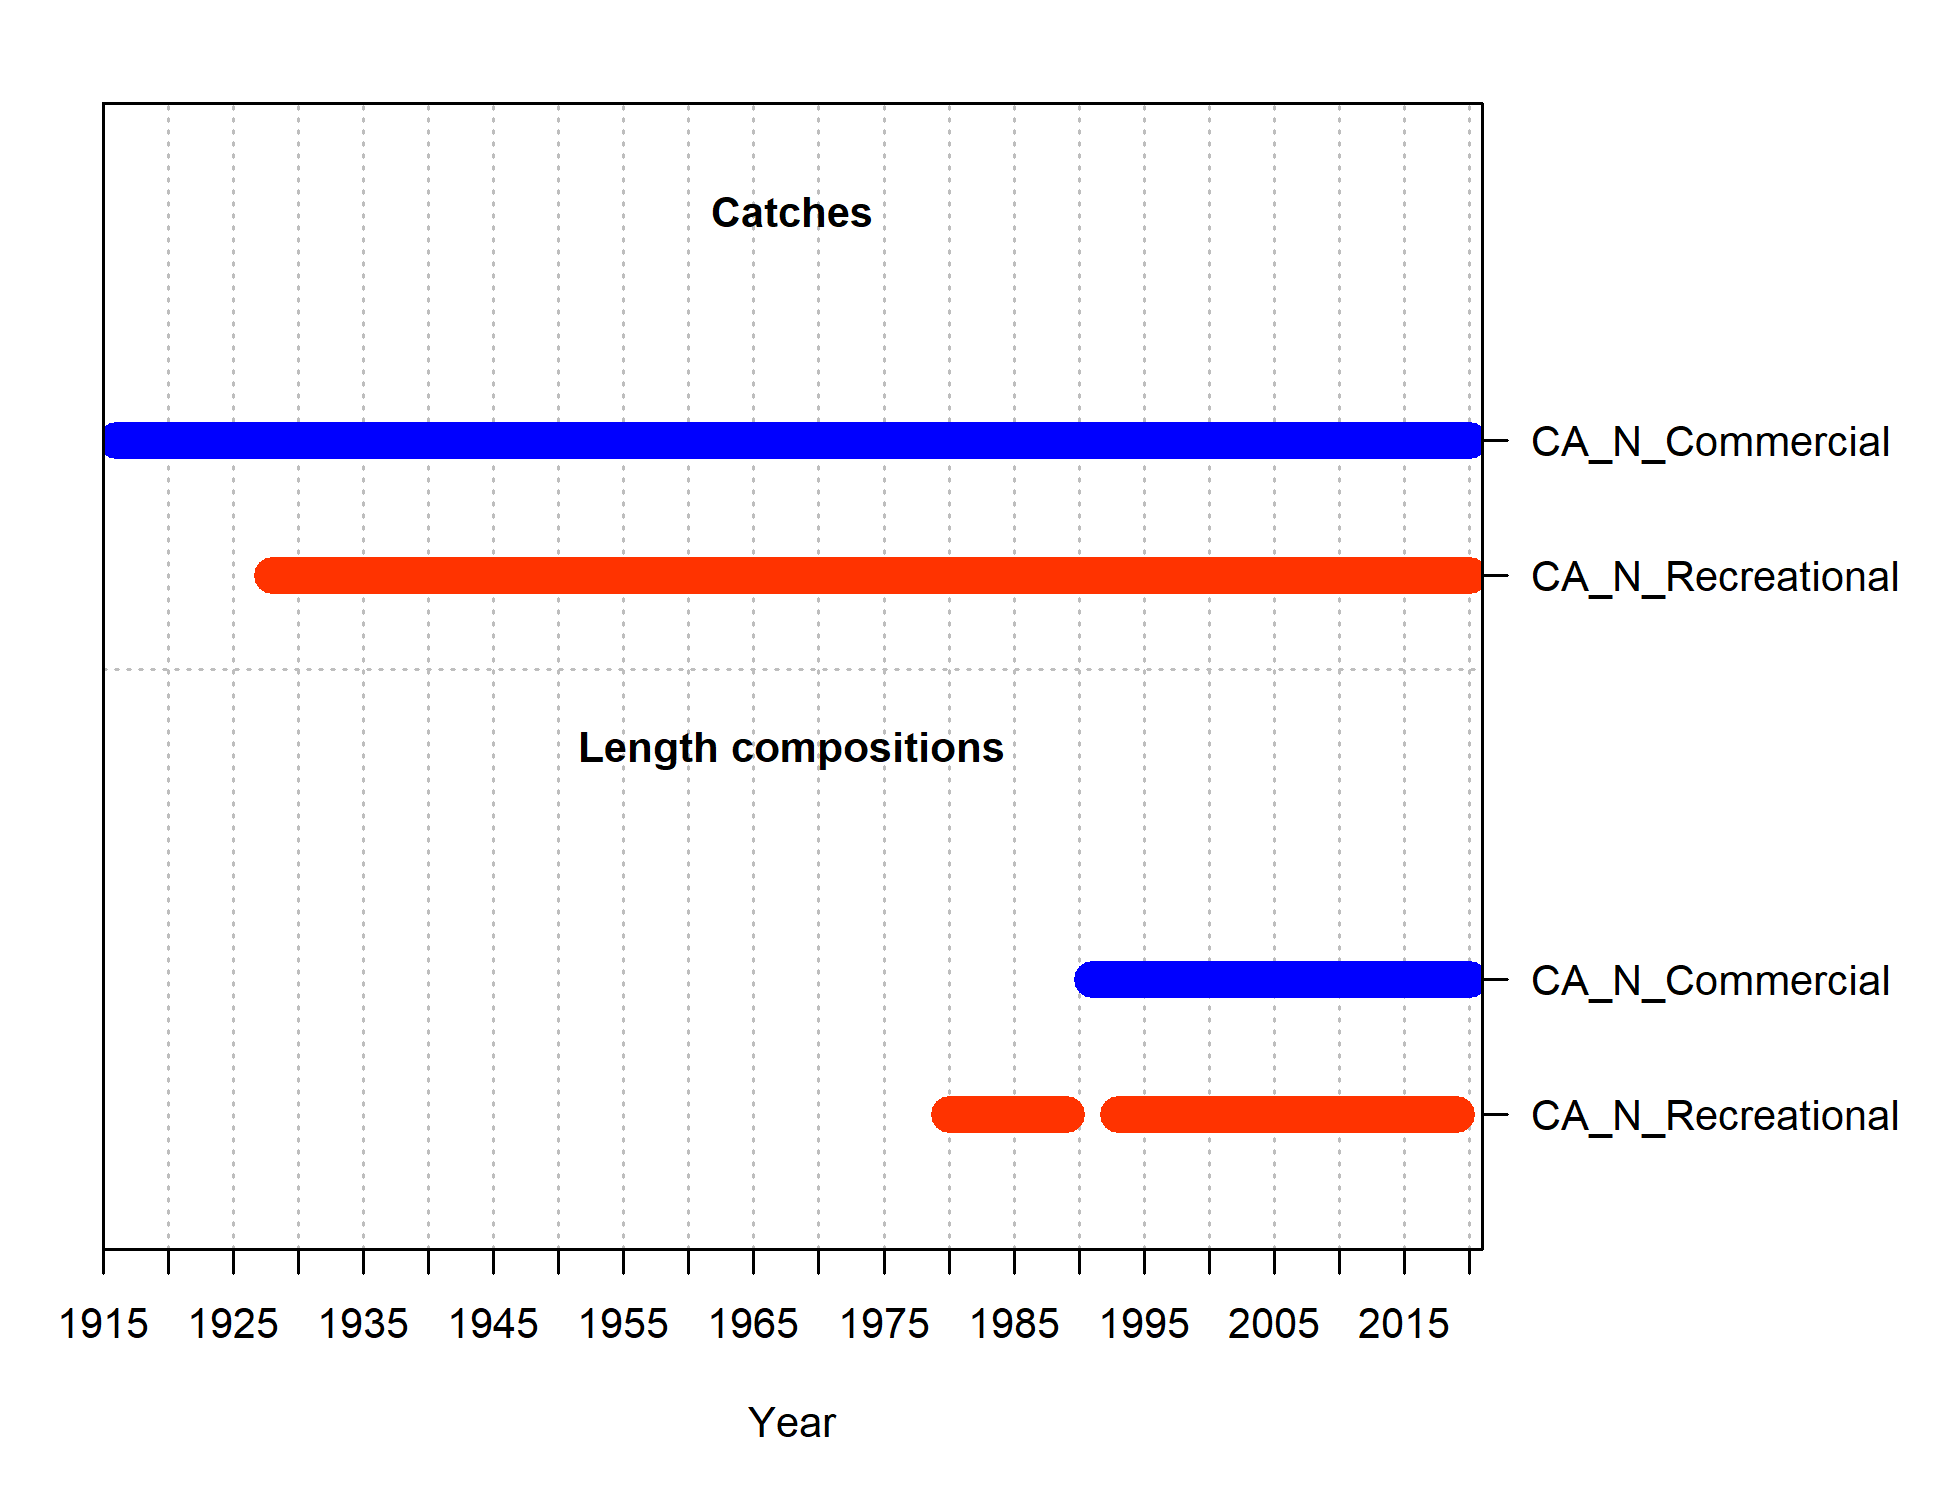
\includegraphics[width=1\textwidth,height=1\textheight]{C:/Assessments/2021/copper_rockfish_2021/models/or/7.0_base/plots/data_plot.png}
\caption{Summary of data sources used in the base model.\label{fig:data-plot}}
\end{figure}

\tagmcend\tagstructend

\tagstructbegin{tag=Figure,alttext={Length composition data from the commercial fleet.}}\tagmcbegin{tag=Figure}

\begin{figure}
\centering
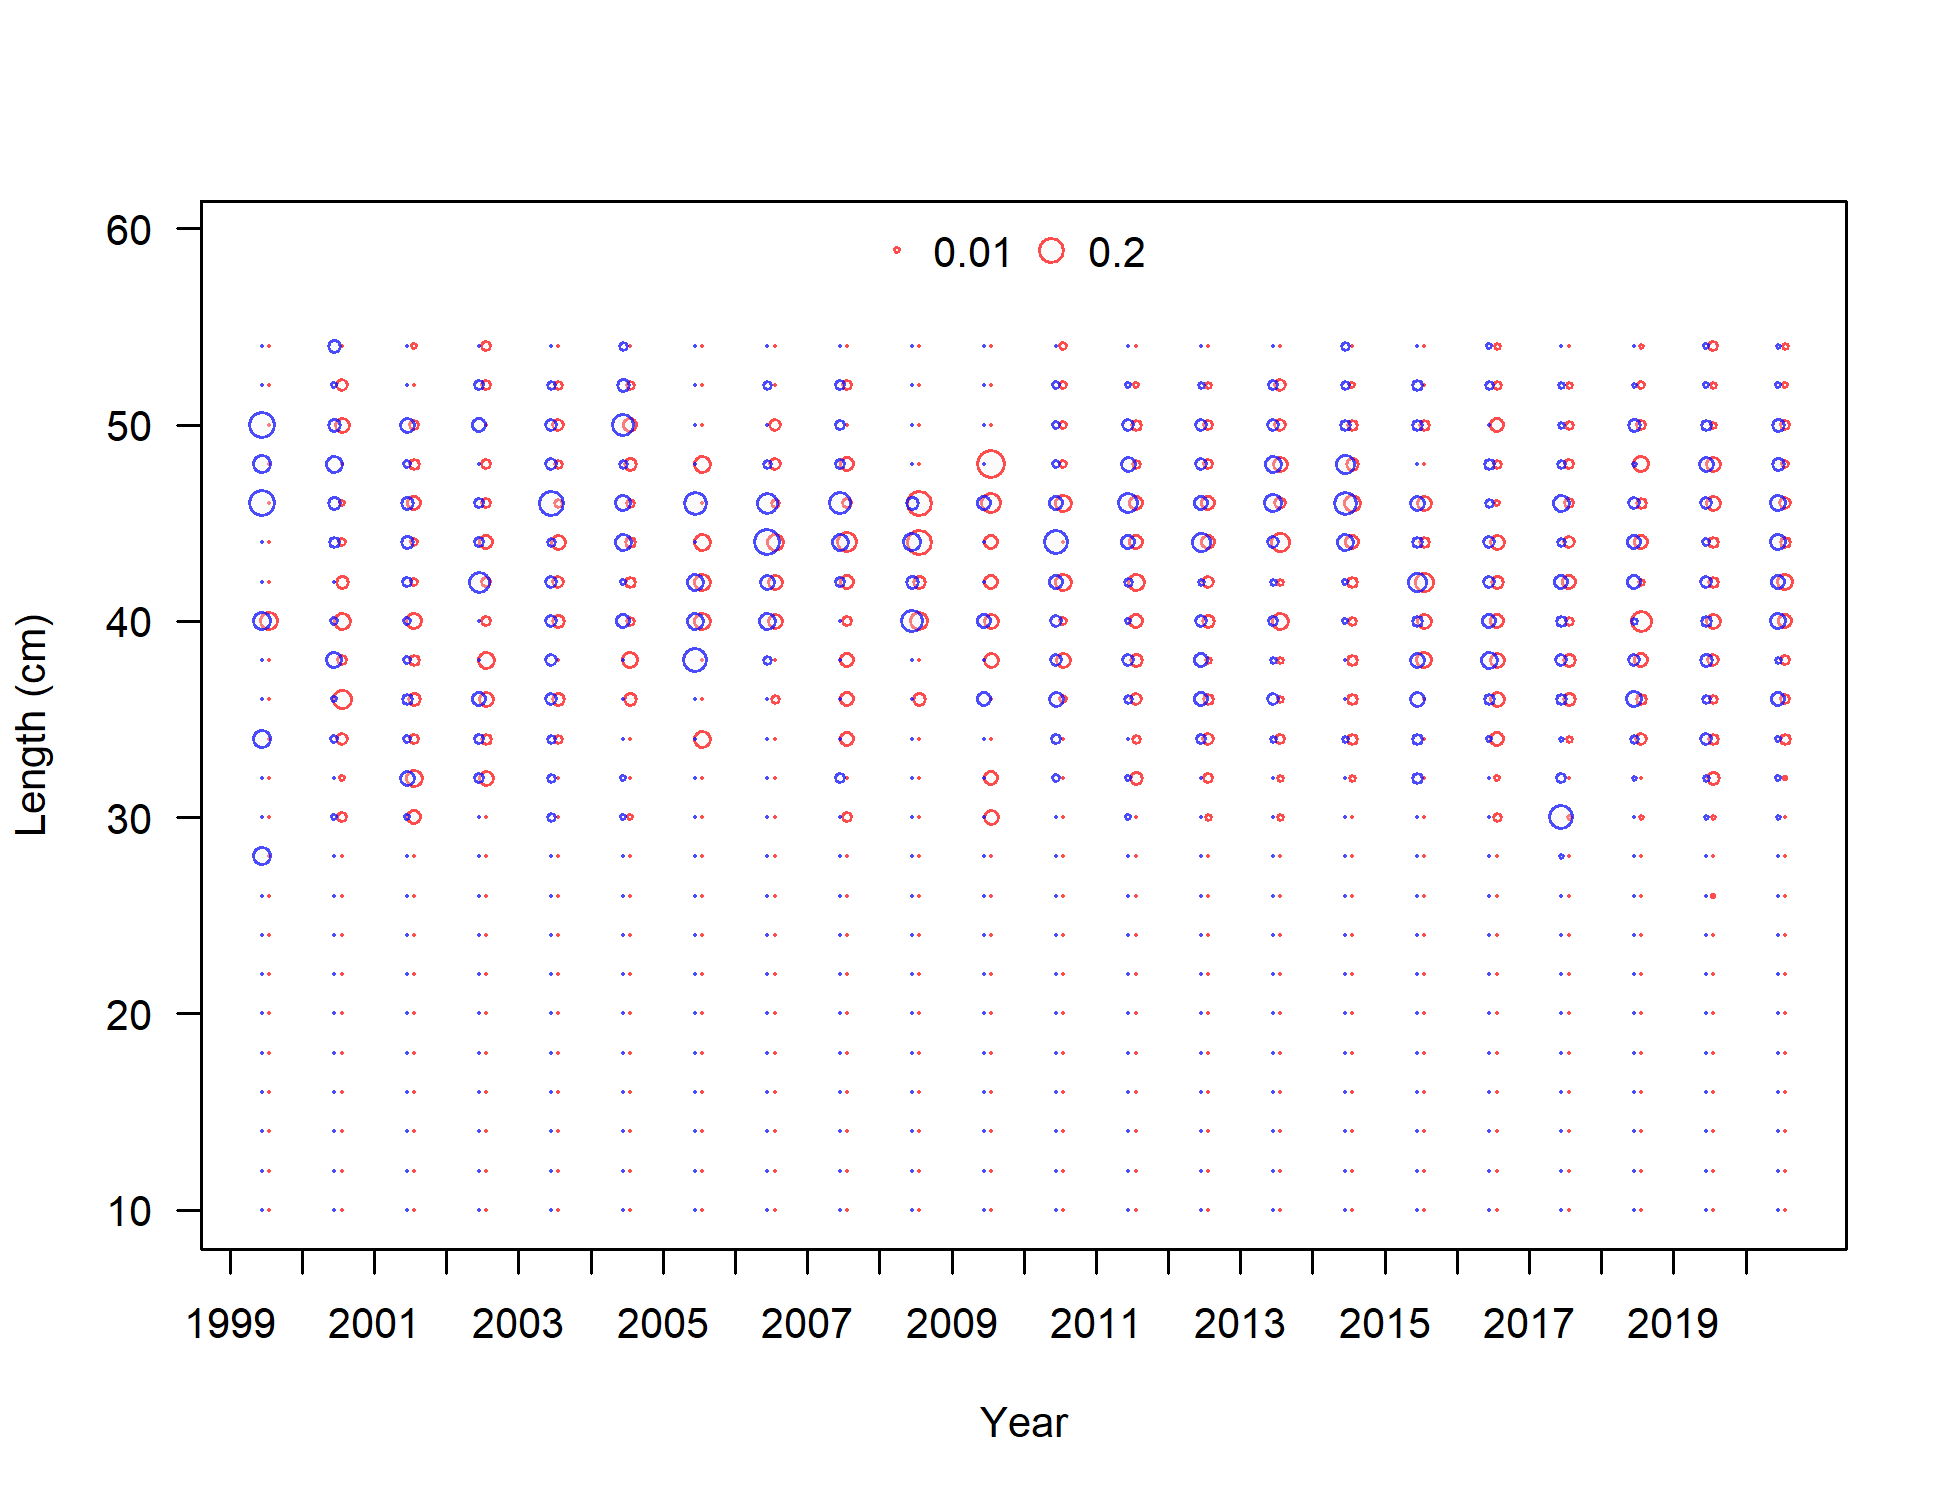
\includegraphics[width=1\textwidth,height=1\textheight]{C:/Assessments/2021/copper_rockfish_2021/models/or/7.0_base/plots/comp_lendat_bubflt1mkt0_page2.png}
\caption{Length composition data from the commercial fleet.\label{fig:com-len-data}}
\end{figure}

\tagmcend\tagstructend

\tagstructbegin{tag=Figure,alttext={Mean length for commercial fleet with 95 percent confidence intervals.}}\tagmcbegin{tag=Figure}

\begin{figure}
\centering
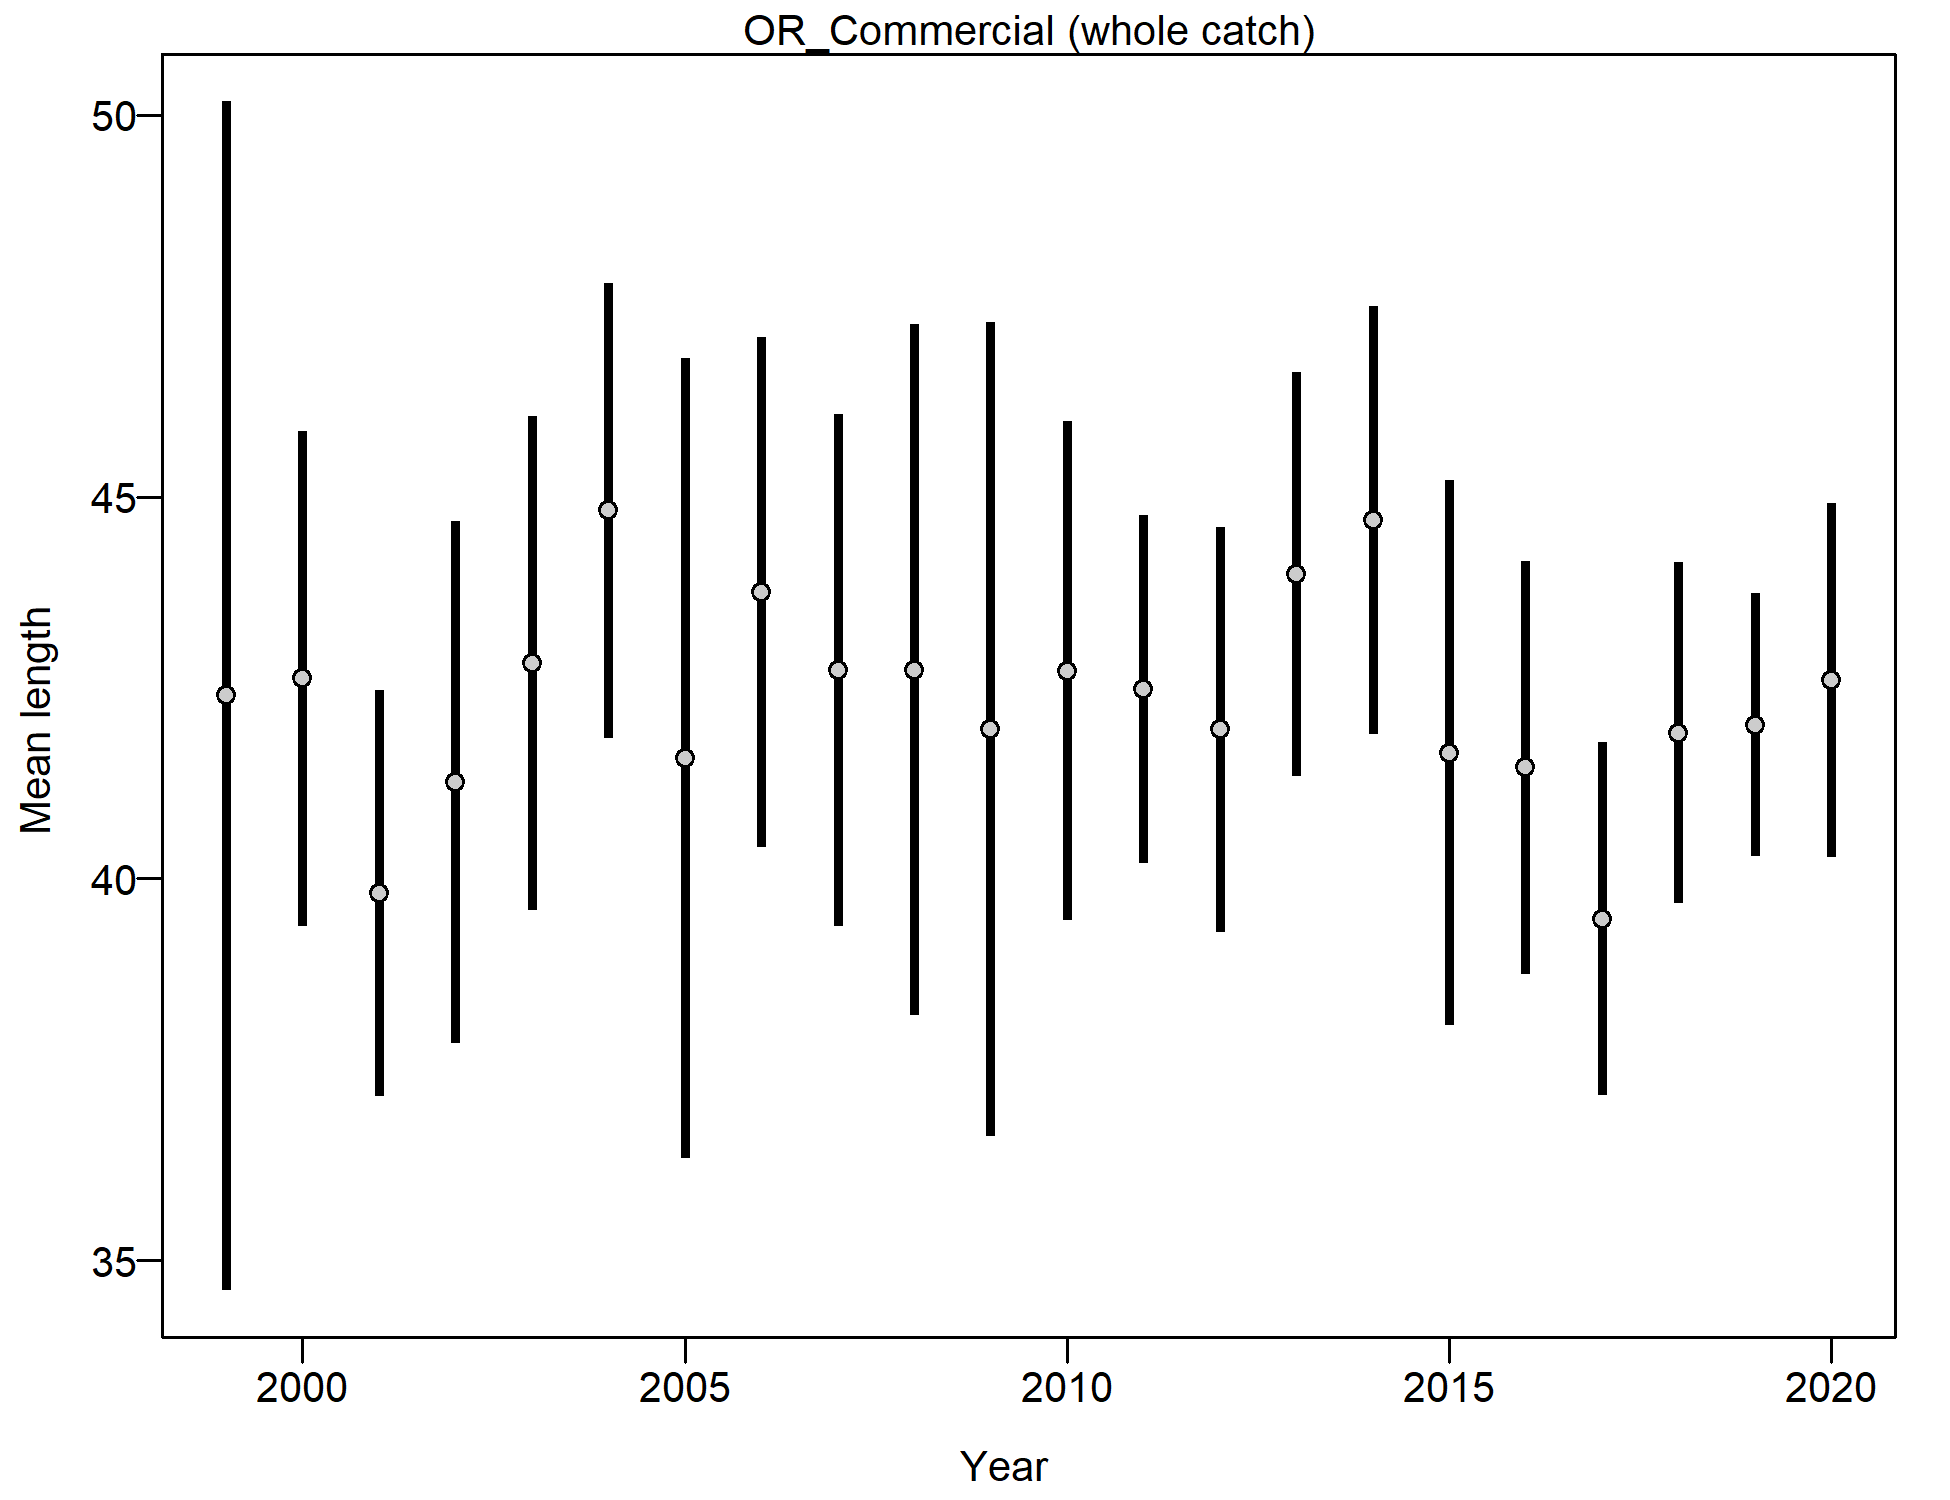
\includegraphics[width=1\textwidth,height=1\textheight]{C:/Assessments/2021/copper_rockfish_2021/models/or/7.0_base/plots/comp_lendat_data_weighting_TA1.8_OR_Commercial.png}
\caption{Mean length for commercial fleet with 95 percent confidence intervals.\label{fig:mean-com-len-data}}
\end{figure}

\tagmcend\tagstructend

\tagstructbegin{tag=Figure,alttext={Length composition data from the recreational fleet.}}\tagmcbegin{tag=Figure}

\begin{figure}
\centering
\includegraphics[width=1\textwidth,height=1\textheight]{C:/Assessments/2021/copper_rockfish_2021/models/or/7.0_base/plots/comp_lendat_bubflt2mkt0_page2.png}
\caption{Length composition data from the recreational fleet.\label{fig:rec-len-data}}
\end{figure}

\tagmcend\tagstructend

\tagstructbegin{tag=Figure,alttext={Mean length for recreational fleet with 95 percent confidence intervals.}}\tagmcbegin{tag=Figure}

\begin{figure}
\centering
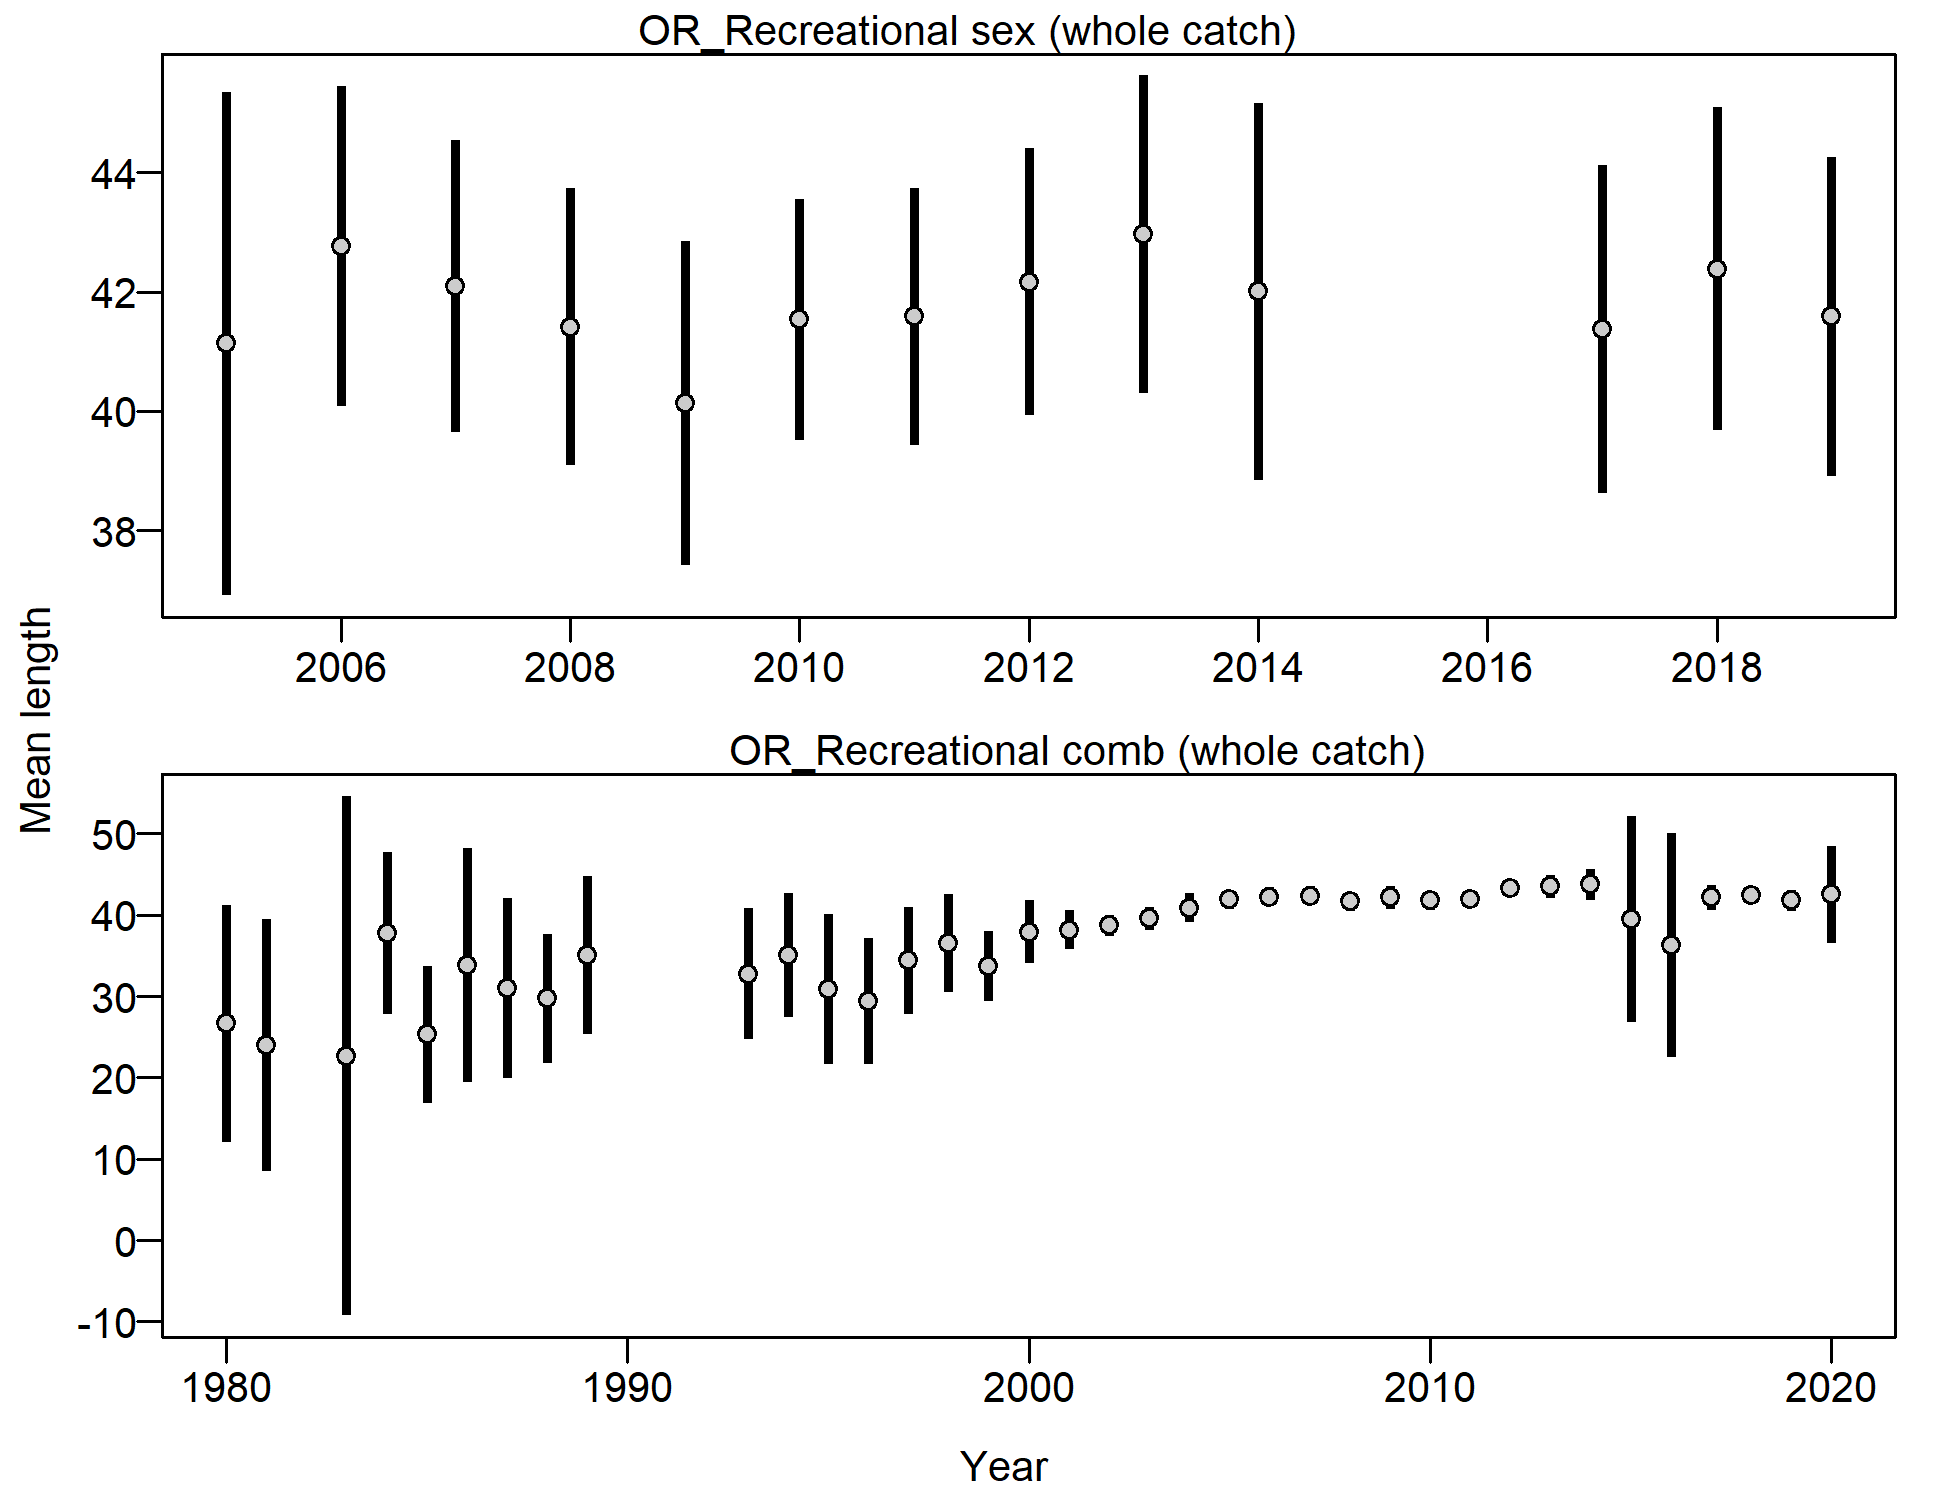
\includegraphics[width=1\textwidth,height=1\textheight]{C:/Assessments/2021/copper_rockfish_2021/models/or/7.0_base/plots/comp_lendat_data_weighting_TA1.8_OR_Recreational.png}
\caption{Mean length for recreational fleet with 95 percent confidence intervals.\label{fig:mean-rec-len-data}}
\end{figure}

\tagmcend\tagstructend

\tagstructbegin{tag=Figure,alttext={Comparison of the length-at-weight data from the NWFSC Hook and Line and the NWFSC WCGBT surveys.}}\tagmcbegin{tag=Figure}

\begin{figure}
\centering
\includegraphics[width=1\textwidth,height=1\textheight]{//nwcfile/FRAM/Assessments/CurrentAssessments/DataModerate_2021/copper_rockfish/data/biology/plots/doc_Length_Weight_Source.png}
\caption{Comparison of the length-at-weight data from the NWFSC Hook and Line and the NWFSC WCGBT surveys.\label{fig:len-weight-survey}}
\end{figure}

\tagmcend\tagstructend

\tagstructbegin{tag=Figure,alttext={Weight-at-length by sex used in the model.}}\tagmcbegin{tag=Figure}

\begin{figure}
\centering
\includegraphics[width=1\textwidth,height=1\textheight]{C:/Assessments/2021/copper_rockfish_2021/models/or/7.0_base/plots/bio5_weightatsize.png}
\caption{Weight-at-length by sex used in the model.\label{fig:len-weight}}
\end{figure}

\tagmcend\tagstructend

\tagstructbegin{tag=Figure,alttext={Observed sex specific length-at-age by data source with the estimate length-at-age curve.}}\tagmcbegin{tag=Figure}

\begin{figure}
\centering
\includegraphics[width=1\textwidth,height=1\textheight]{//nwcfile/FRAM/Assessments/CurrentAssessments/DataModerate_2021/copper_rockfish/data/biology/plots/doc_north_Age_by_Sex_Source.png}
\caption{Observed sex specific length-at-age by data source with the estimate length-at-age curve.\label{fig:len-age-data}}
\end{figure}

\tagmcend\tagstructend

\tagstructbegin{tag=Figure,alttext={Length at age in the beginning of the year in the ending year of the model.}}\tagmcbegin{tag=Figure}

\begin{figure}
\centering
\includegraphics[width=1\textwidth,height=1\textheight]{C:/Assessments/2021/copper_rockfish_2021/models/or/7.0_base/plots/bio1_sizeatage.png}
\caption{Length at age in the beginning of the year in the ending year of the model.\label{fig:len-age-ss}}
\end{figure}

\tagmcend\tagstructend

\tagstructbegin{tag=Figure,alttext={Maturity as a function of  length.}}\tagmcbegin{tag=Figure}

\begin{figure}
\centering
\includegraphics[width=1\textwidth,height=1\textheight]{C:/Assessments/2021/copper_rockfish_2021/models/or/7.0_base/plots/bio6_maturity.png}
\caption{Maturity as a function of length.\label{fig:maturity}}
\end{figure}

\tagmcend\tagstructend

\tagstructbegin{tag=Figure,alttext={Fecundity as a function of length.}}\tagmcbegin{tag=Figure}

\begin{figure}
\centering
\includegraphics[width=1\textwidth,height=1\textheight]{C:/Assessments/2021/copper_rockfish_2021/models/or/7.0_base/plots/bio9_fecundity_len.png}
\caption{Fecundity as a function of length.\label{fig:fecundity}}
\end{figure}

\tagmcend\tagstructend

\tagstructbegin{tag=Figure,alttext={Fraction female by length across all available data sources.}}\tagmcbegin{tag=Figure}

\begin{figure}
\centering
\includegraphics[width=1\textwidth,height=1\textheight]{//nwcfile/FRAM/Assessments/CurrentAssessments/DataModerate_2021/copper_rockfish/data/biology/plots/Length_fraction_female.png}
\caption{Fraction female by length across all available data sources.\label{fig:len-sex-ratio}}
\end{figure}

\tagmcend\tagstructend

\tagstructbegin{tag=Figure,alttext={Fraction female by age across all available data sources.}}\tagmcbegin{tag=Figure}

\begin{figure}
\centering
\includegraphics[width=1\textwidth,height=1\textheight]{//nwcfile/FRAM/Assessments/CurrentAssessments/DataModerate_2021/copper_rockfish/data/biology/plots/Age_fraction_female.png}
\caption{Fraction female by age across all available data sources.\label{fig:age-sex-ratio}}
\end{figure}

\tagmcend\tagstructend

\tagstructbegin{tag=Figure,alttext={Selectivity at length by fleet.}}\tagmcbegin{tag=Figure}

\begin{figure}
\centering
\includegraphics[width=1\textwidth,height=1\textheight]{C:/Assessments/2021/copper_rockfish_2021/models/or/7.0_base/plots/sel01_multiple_fleets_length1.png}
\caption{Selectivity at length by fleet.\label{fig:selex}}
\end{figure}

\tagmcend\tagstructend

\tagstructbegin{tag=Figure,alttext={Estimated time series of age-0 recruits (1000s).}}\tagmcbegin{tag=Figure}

\begin{figure}
\centering
\includegraphics[width=1\textwidth,height=1\textheight]{C:/Assessments/2021/copper_rockfish_2021/models/or/7.0_base/plots/ts11_Age-0_recruits_(1000s)_with_95_asymptotic_intervals.png}
\caption{Estimated time series of age-0 recruits (1000s).\label{fig:recruits}}
\end{figure}

\tagmcend\tagstructend

\tagstructbegin{tag=Figure,alttext={Estimated time series of recruitment deviations.}}\tagmcbegin{tag=Figure}

\begin{figure}
\centering
\includegraphics[width=1\textwidth,height=1\textheight]{C:/Assessments/2021/copper_rockfish_2021/models/or/7.0_base/plots/recdevs2_withbars.png}
\caption{Estimated time series of recruitment deviations.\label{fig:rec-devs}}
\end{figure}

\tagmcend\tagstructend

\tagstructbegin{tag=Figure,alttext={Recruitment bias adjustment applied in the base model.}}\tagmcbegin{tag=Figure}

\begin{figure}
\centering
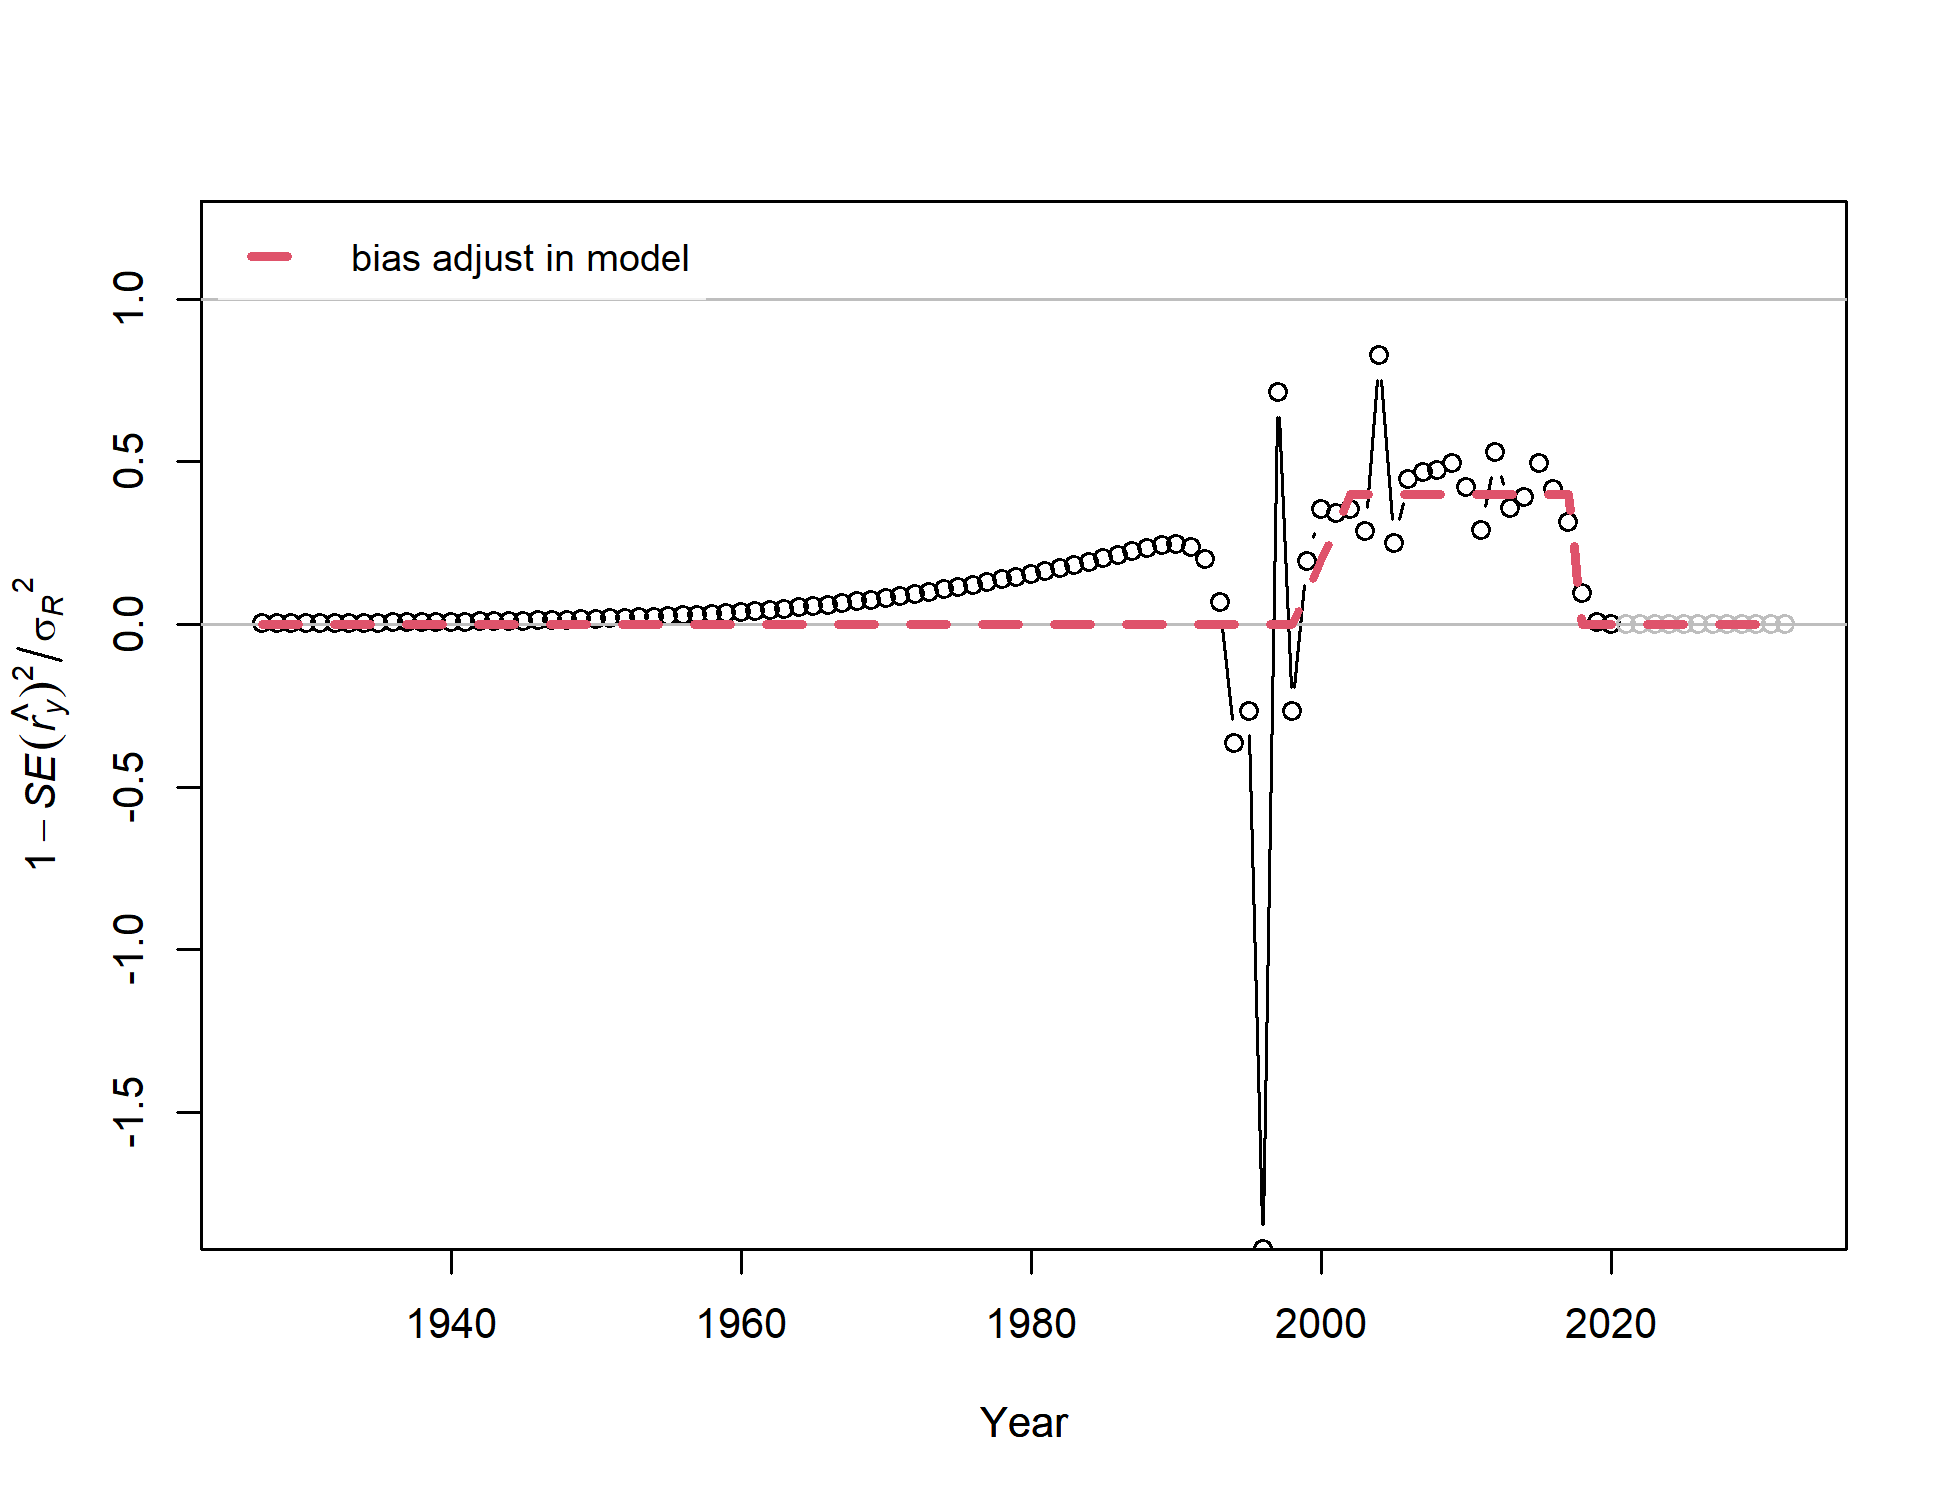
\includegraphics[width=1\textwidth,height=1\textheight]{C:/Assessments/2021/copper_rockfish_2021/write_up/or/figs/recruit_fit_bias_adjust.png}
\caption{Recruitment bias adjustment applied in the base model.\label{fig:bias-adj}}
\end{figure}

\tagmcend\tagstructend

\tagstructbegin{tag=Figure,alttext={Pearson residuals for commercial fleet. Closed bubble are positive residuals (observed > expected) and open bubbles are negative residuals (observed < expected).}}\tagmcbegin{tag=Figure}

\begin{figure}
\centering
\includegraphics[width=1\textwidth,height=1\textheight]{C:/Assessments/2021/copper_rockfish_2021/models/or/7.0_base/plots/comp_lenfit_residsflt1mkt0_page2.png}
\caption{Pearson residuals for commercial fleet. Closed bubble are positive residuals (observed \textgreater{} expected) and open bubbles are negative residuals (observed \textless{} expected).\label{fig:com-pearson}}
\end{figure}

\tagmcend\tagstructend

\tagstructbegin{tag=Figure,alttext={Mean length for commercial lengths with 95 percent confidence intervals based on current samples sizes.}}\tagmcbegin{tag=Figure}

\begin{figure}
\centering
\includegraphics[width=1\textwidth,height=1\textheight]{C:/Assessments/2021/copper_rockfish_2021/models/or/7.0_base/plots/comp_lenfit_data_weighting_TA1.8_OR_Commercial.png}
\caption{Mean length for commercial lengths with 95 percent confidence intervals based on current samples sizes.\label{fig:com-mean-len-fit}}
\end{figure}

\tagmcend\tagstructend

\tagstructbegin{tag=Figure,alttext={Pearson residuals for recreational fleet. Closed bubble are positive residuals (observed > expected) and open bubbles are negative residuals (observed < expected).}}\tagmcbegin{tag=Figure}

\begin{figure}
\centering
\includegraphics[width=1\textwidth,height=1\textheight]{C:/Assessments/2021/copper_rockfish_2021/models/or/7.0_base/plots/comp_lenfit_residsflt2mkt0_page2.png}
\caption{Pearson residuals for recreational fleet. Closed bubble are positive residuals (observed \textgreater{} expected) and open bubbles are negative residuals (observed \textless{} expected).\label{fig:rec-pearson}}
\end{figure}

\tagmcend\tagstructend

\tagstructbegin{tag=Figure,alttext={Mean length for recreational lengths with 95 percent confidence intervals based on current samples sizes.}}\tagmcbegin{tag=Figure}

\begin{figure}
\centering
\includegraphics[width=1\textwidth,height=1\textheight]{C:/Assessments/2021/copper_rockfish_2021/models/or/7.0_base/plots/comp_lenfit_data_weighting_TA1.8_OR_Recreational.png}
\caption{Mean length for recreational lengths with 95 percent confidence intervals based on current samples sizes.\label{fig:rec-mean-len-fit}}
\end{figure}

\tagmcend\tagstructend

\tagstructbegin{tag=Figure,alttext={Aggregated length comps over all years.}}\tagmcbegin{tag=Figure}

\begin{figure}
\centering
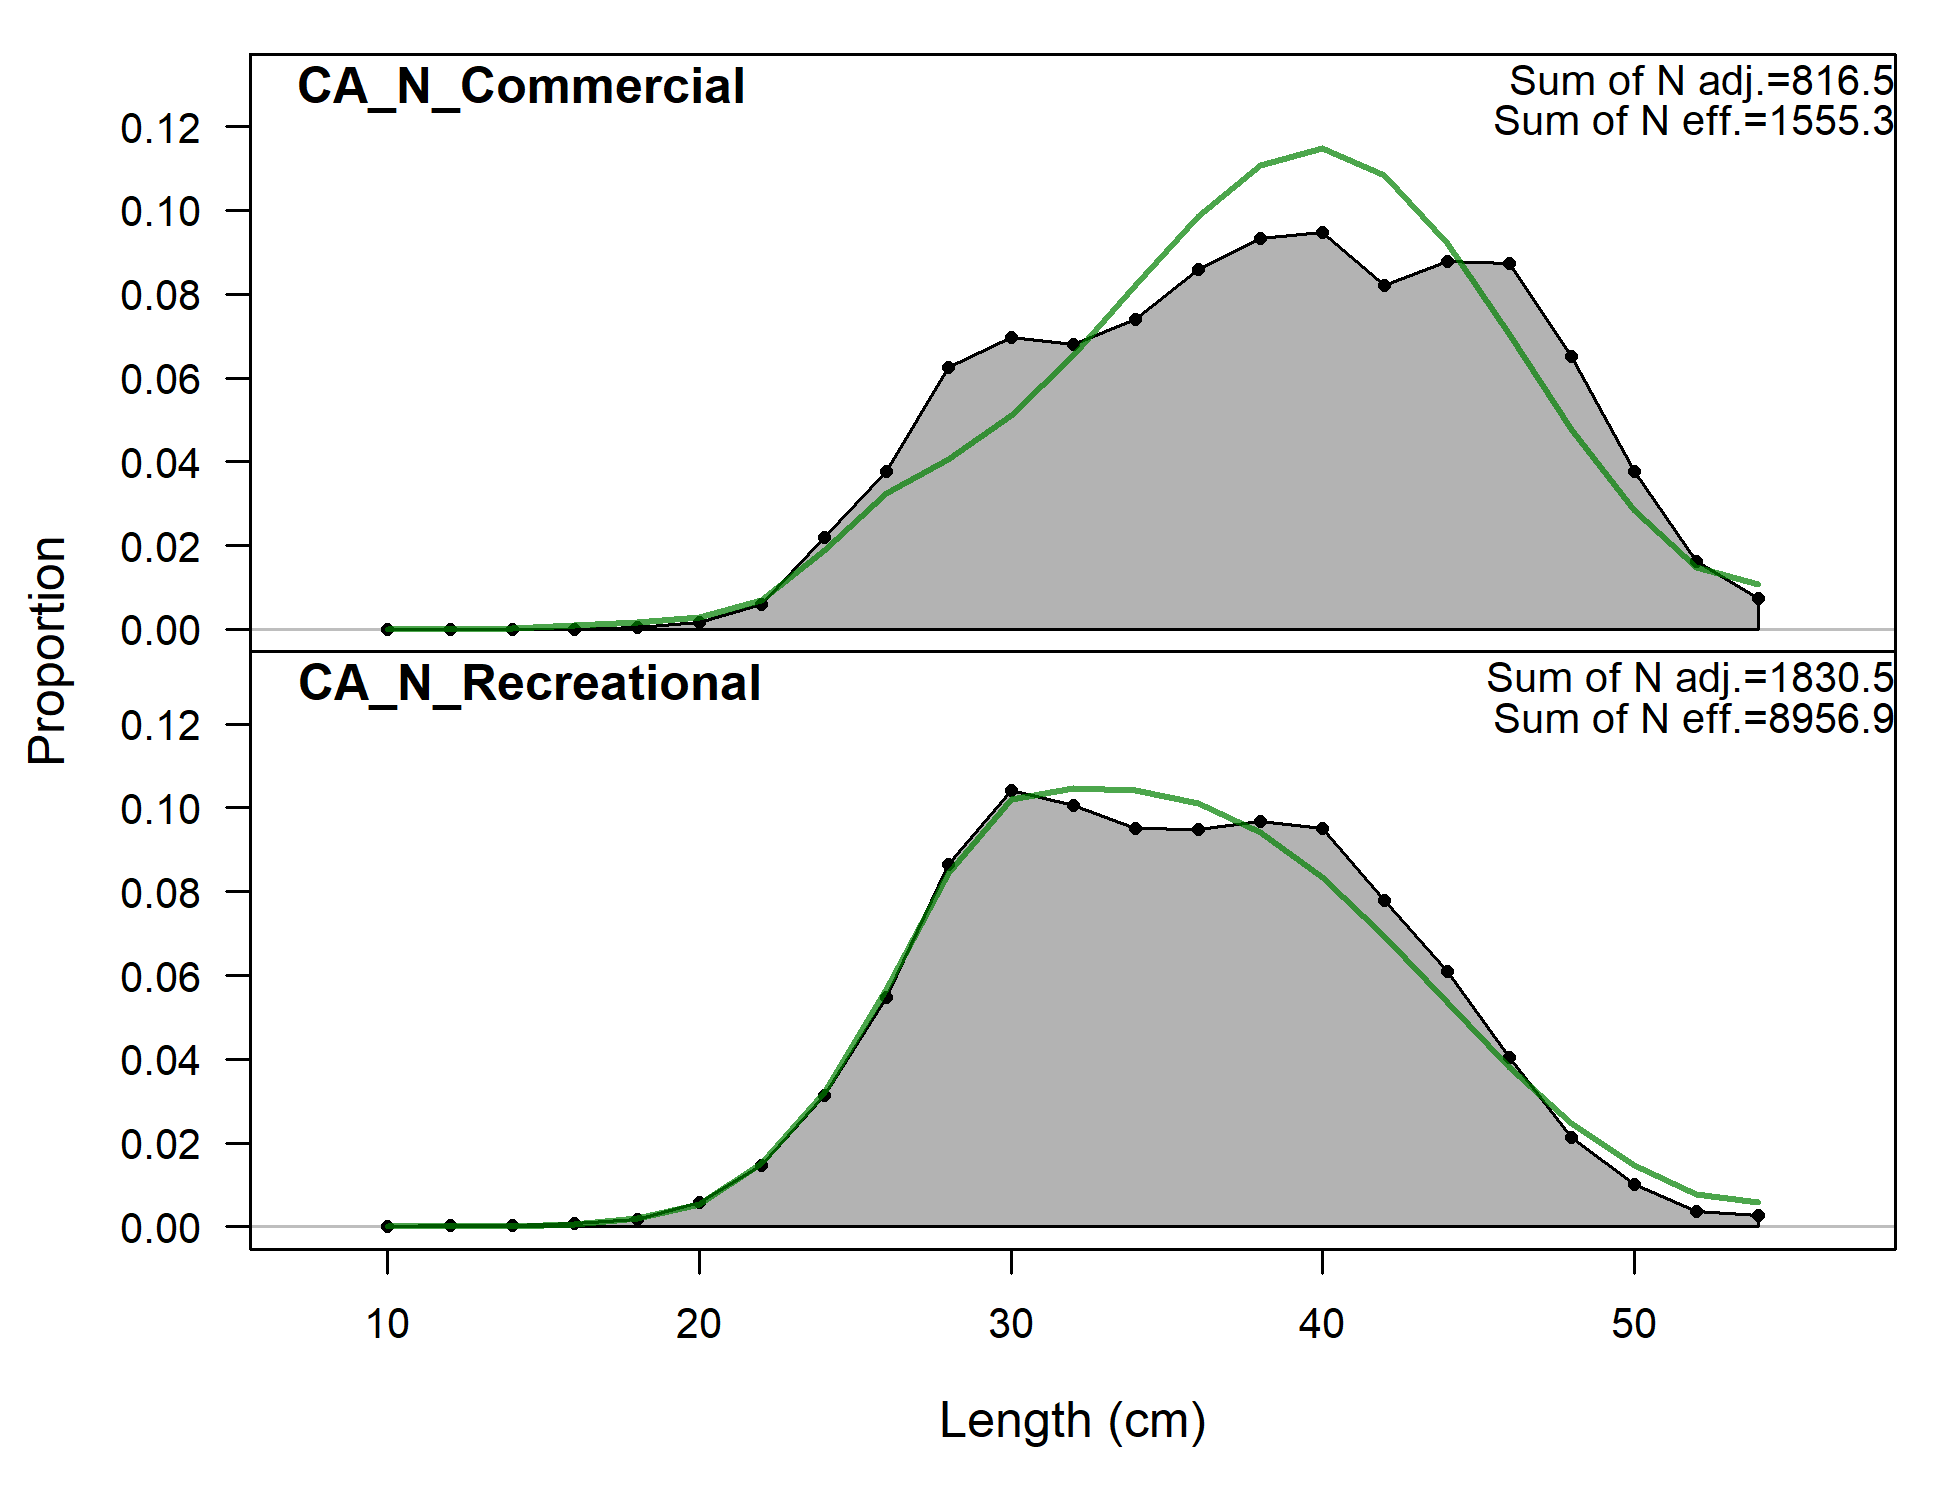
\includegraphics[width=1\textwidth,height=1\textheight]{C:/Assessments/2021/copper_rockfish_2021/models/or/7.0_base/plots/comp_lenfit__aggregated_across_time.png}
\caption{Aggregated length comps over all years.\label{fig:agg-len-fit}}
\end{figure}

\tagmcend\tagstructend

\tagstructbegin{tag=Figure,alttext={Estimated time series of spawning output.}}\tagmcbegin{tag=Figure}

\begin{figure}
\centering
\includegraphics[width=1\textwidth,height=1\textheight]{C:/Assessments/2021/copper_rockfish_2021/models/or/7.0_base/plots/ts7_Spawning_output_with_95_asymptotic_intervals_intervals.png}
\caption{Estimated time series of spawning output.\label{fig:ssb}}
\end{figure}

\tagmcend\tagstructend

\tagstructbegin{tag=Figure,alttext={Estimated time series of total biomass.}}\tagmcbegin{tag=Figure}

\begin{figure}
\centering
\includegraphics[width=1\textwidth,height=1\textheight]{C:/Assessments/2021/copper_rockfish_2021/models/or/7.0_base/plots/ts1_Total_biomass_(mt).png}
\caption{Estimated time series of total biomass.\label{fig:tot-bio}}
\end{figure}

\tagmcend\tagstructend

\tagstructbegin{tag=Figure,alttext={Estimated time series of relative spawning output.}}\tagmcbegin{tag=Figure}

\begin{figure}
\centering
\includegraphics[width=1\textwidth,height=1\textheight]{C:/Assessments/2021/copper_rockfish_2021/models/or/7.0_base/plots/ts9_Relative_spawning_output_intervals.png}
\caption{Estimated time series of relative spawning output.\label{fig:depl}}
\end{figure}

\tagmcend\tagstructend

\tagstructbegin{tag=Figure,alttext={Proportion of biomass unavailable due to selectivity for small and large fish..}}\tagmcbegin{tag=Figure}

\begin{figure}
\centering
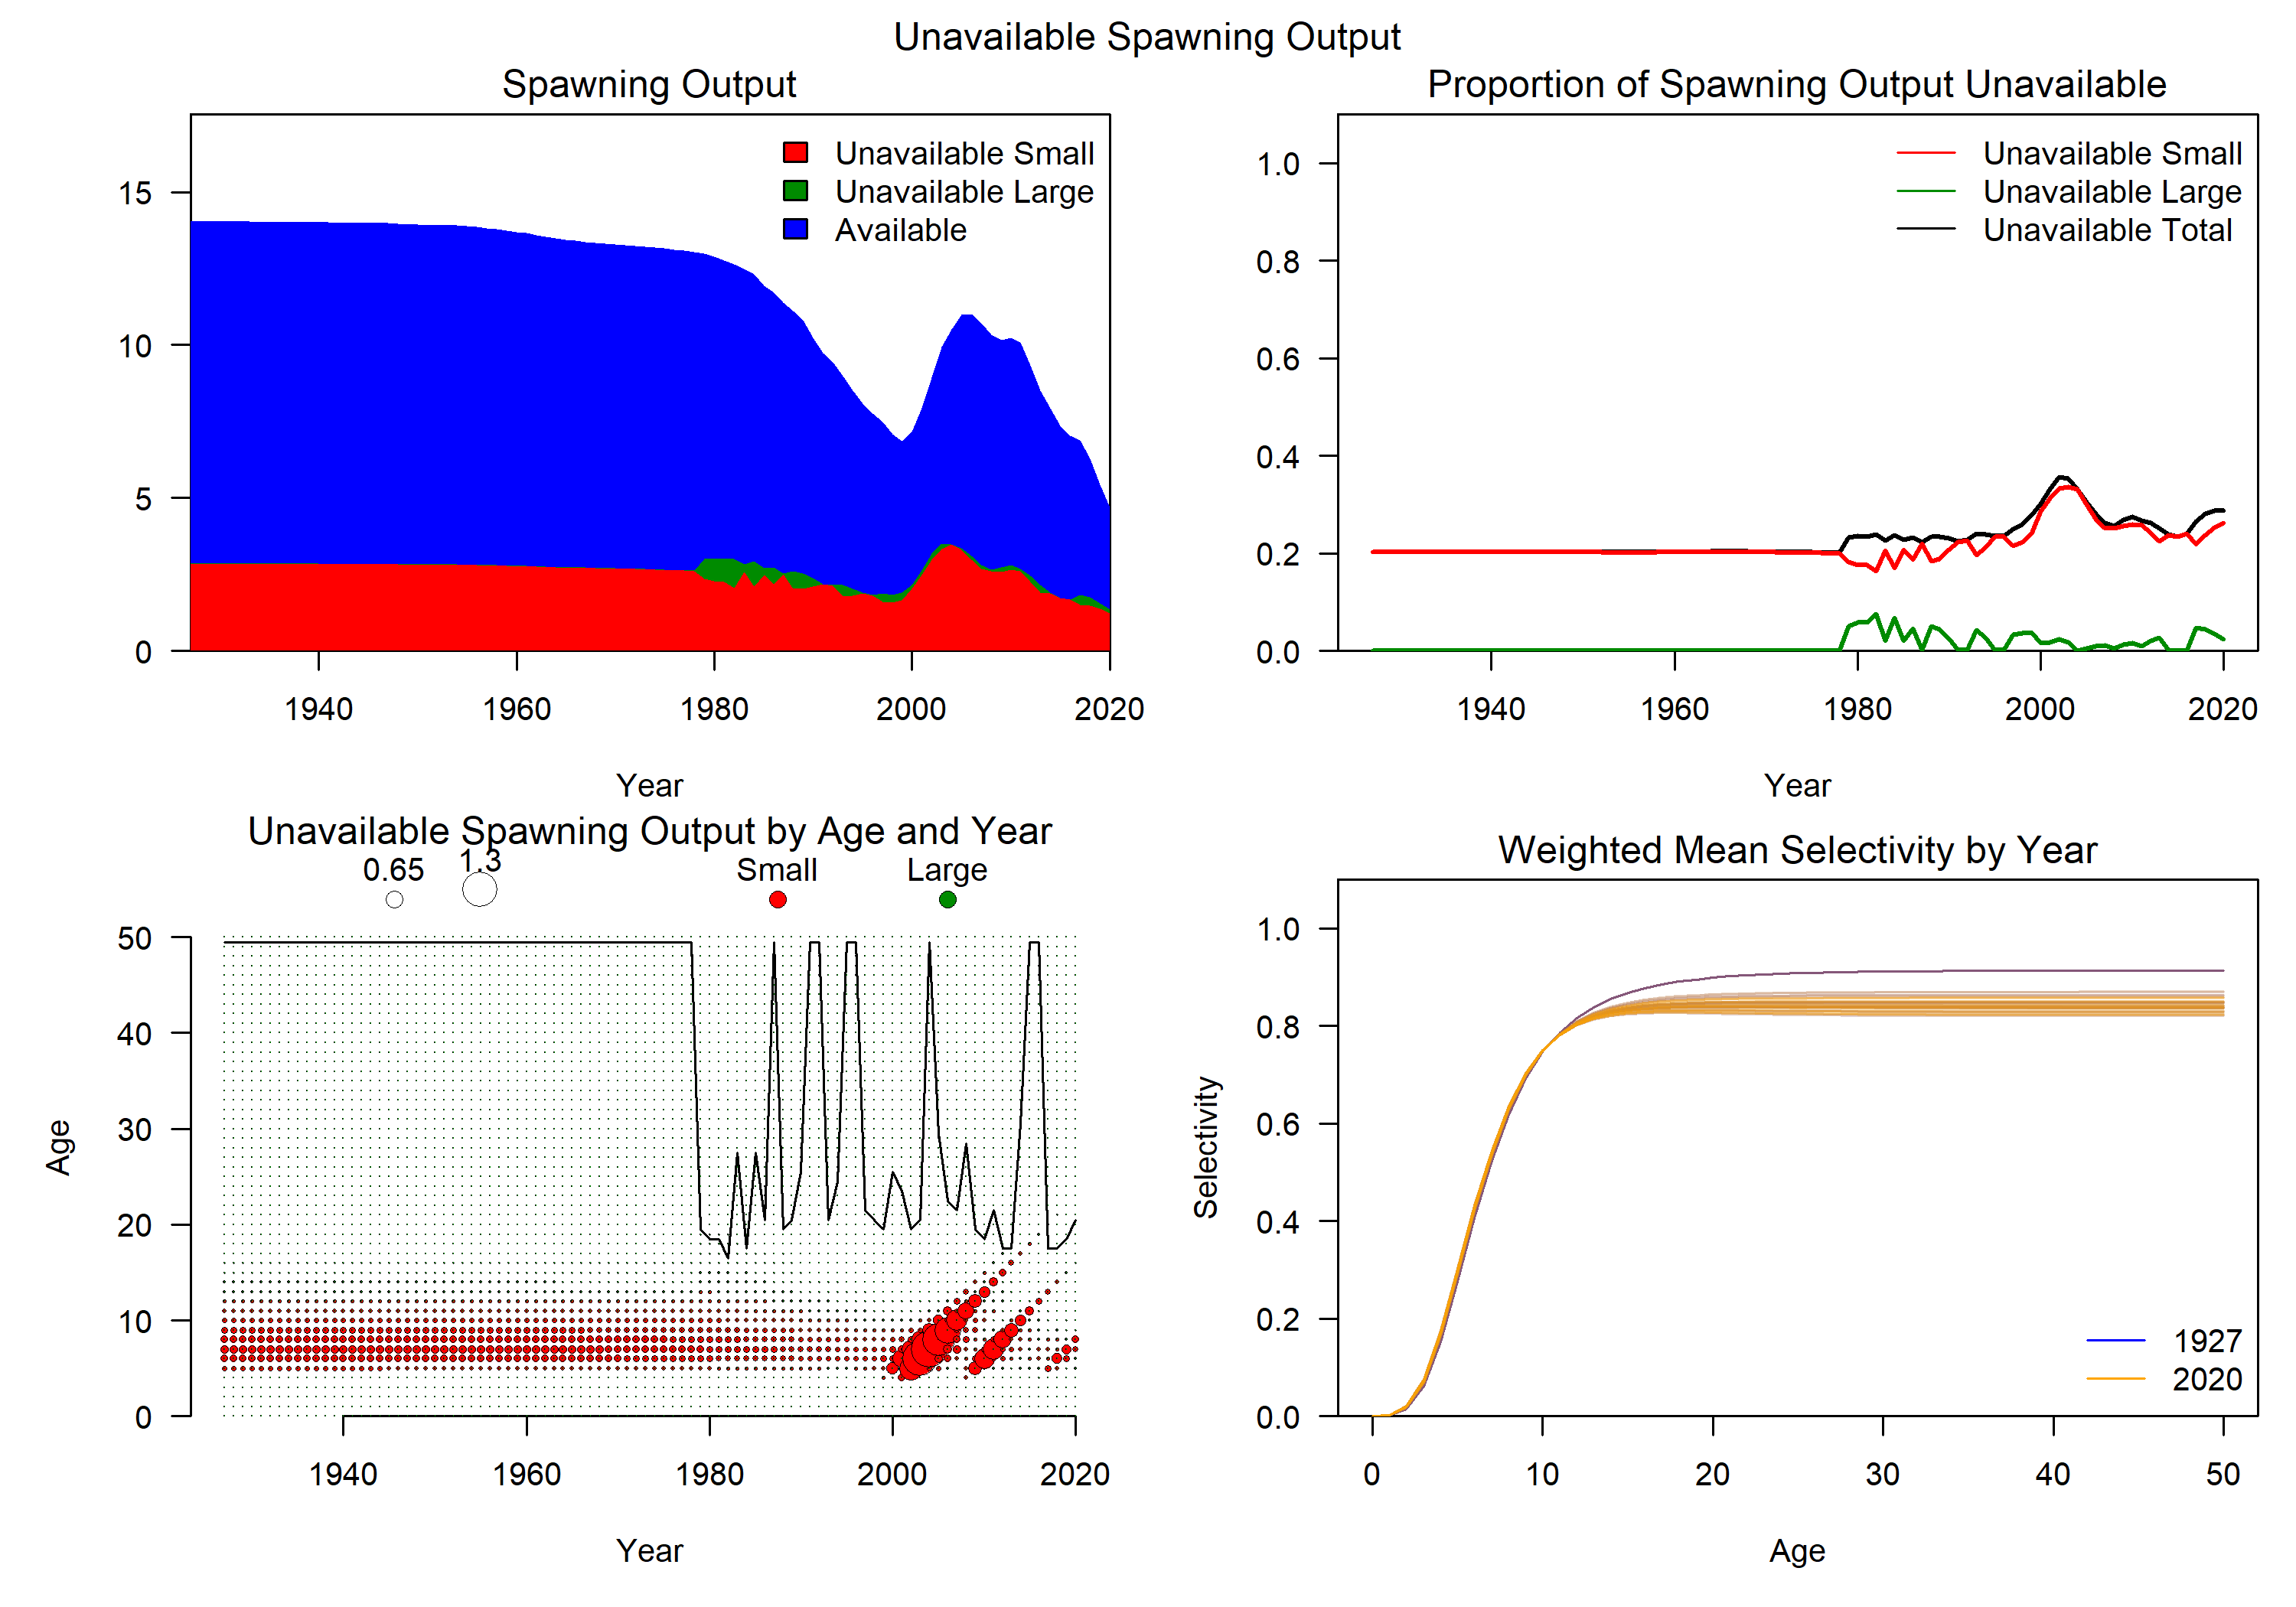
\includegraphics[width=1\textwidth,height=1\textheight]{C:/Assessments/2021/copper_rockfish_2021/write_up/or/figs/unavailable_biomass.png}
\caption{Proportion of biomass unavailable due to selectivity for small and large fish..\label{fig:unavail-bio}}
\end{figure}

\tagmcend\tagstructend

\tagstructbegin{tag=Figure,alttext={Stock-recruit curve. Point colors indicate year, with warmer colors indicating earlier years and cooler colors in showing later years.}}\tagmcbegin{tag=Figure}

\begin{figure}
\centering
\includegraphics[width=1\textwidth,height=1\textheight]{C:/Assessments/2021/copper_rockfish_2021/models/or/7.0_base/plots/SR_curve.png}
\caption{Stock-recruit curve. Point colors indicate year, with warmer colors indicating earlier years and cooler colors in showing later years.\label{fig:bh-curve}}
\end{figure}

\tagmcend\tagstructend

\tagstructbegin{tag=Figure,alttext={Estimated 1 - relative spawning ratio (SPR) by year.}}\tagmcbegin{tag=Figure}

\begin{figure}
\centering
\includegraphics[width=1\textwidth,height=1\textheight]{C:/Assessments/2021/copper_rockfish_2021/models/or/7.0_base/plots/SPR2_minusSPRseries.png}
\caption{Estimated 1 - relative spawning ratio (SPR) by year.\label{fig:1-spr}}
\end{figure}

\tagmcend\tagstructend

\tagstructbegin{tag=Figure,alttext={Equilibrium yield curve for the base case model. Values are based on the 2020 fishery selectivity and with steepness fixed at 0.72.}}\tagmcbegin{tag=Figure}

\begin{figure}
\centering
\includegraphics[width=1\textwidth,height=1\textheight]{C:/Assessments/2021/copper_rockfish_2021/models/or/7.0_base/plots/yield2_yield_curve_with_refpoints.png}
\caption{Equilibrium yield curve for the base case model. Values are based on the 2020 fishery selectivity and with steepness fixed at 0.72.\label{fig:yield}}
\end{figure}

\tagmcend\tagstructend

\tagstructbegin{tag=Figure,alttext={Change in estimated spawning output by sensitivity.}}\tagmcbegin{tag=Figure}

\begin{figure}
\centering
\includegraphics[width=1\textwidth,height=1\textheight]{C:/Assessments/2021/copper_rockfish_2021/models/or/_sensitivities/_plots/7.0_base_compare2_spawnbio_uncertainty.png}
\caption{Change in estimated spawning output by sensitivity.\label{fig:sens-ssb}}
\end{figure}

\tagmcend\tagstructend

\tagstructbegin{tag=Figure,alttext={Change in estimated fraction unfished by sensitivity.}}\tagmcbegin{tag=Figure}

\begin{figure}
\centering
\includegraphics[width=1\textwidth,height=1\textheight]{C:/Assessments/2021/copper_rockfish_2021/models/or/_sensitivities/_plots/7.0_base_compare4_Bratio_uncertainty.png}
\caption{Change in estimated fraction unfished by sensitivity.\label{fig:sens-depl}}
\end{figure}

\tagmcend\tagstructend

\tagstructbegin{tag=Figure,alttext={Change in estimated annual recruitment deviation.}}\tagmcbegin{tag=Figure}

\begin{figure}
\centering
\includegraphics[width=1\textwidth,height=1\textheight]{C:/Assessments/2021/copper_rockfish_2021/models/or/_sensitivities/_plots/7.0_base_compare12_recdevs_uncertainty.png}
\caption{Change in estimated annual recruitment deviation.\label{fig:sens-recdev}}
\end{figure}

\tagmcend\tagstructend

\tagstructbegin{tag=Figure,alttext={Change in the negative log-likelihood across a range of log(R0) values.}}\tagmcbegin{tag=Figure}

\begin{figure}
\centering
\includegraphics[width=1\textwidth,height=1\textheight]{C:/Assessments/2021/copper_rockfish_2021/models/or/7.0_base_profile_SR_LN(R0)/piner_panel_SR_LN(R0).png}
\caption{Change in the negative log-likelihood across a range of log(R0) values.\label{fig:r0-profile}}
\end{figure}

\tagmcend\tagstructend

\tagstructbegin{tag=Figure,alttext={Change in the estimate of spawning output across a range of log(R0) values.}}\tagmcbegin{tag=Figure}

\begin{figure}
\centering
\includegraphics[width=1\textwidth,height=1\textheight]{C:/Assessments/2021/copper_rockfish_2021/models/or/7.0_base_profile_SR_LN(R0)/SR_LN(R0)_trajectories_compare1_spawnbio.png}
\caption{Change in the estimate of spawning output across a range of log(R0) values.\label{fig:r0-ssb}}
\end{figure}

\tagmcend\tagstructend

\tagstructbegin{tag=Figure,alttext={Change in the estimate of fraction unfished across a range of log(R0) values.}}\tagmcbegin{tag=Figure}

\begin{figure}
\centering
\includegraphics[width=1\textwidth,height=1\textheight]{C:/Assessments/2021/copper_rockfish_2021/models/or/7.0_base_profile_SR_LN(R0)/SR_LN(R0)_trajectories_compare3_Bratio.png}
\caption{Change in the estimate of fraction unfished across a range of log(R0) values.\label{fig:r0-depl}}
\end{figure}

\tagmcend\tagstructend

\tagstructbegin{tag=Figure,alttext={Change in the negative log-likelihood across a range of steepness values.}}\tagmcbegin{tag=Figure}

\begin{figure}
\centering
\includegraphics[width=1\textwidth,height=1\textheight]{C:/Assessments/2021/copper_rockfish_2021/models/or/7.0_base_profile_SR_BH_steep/piner_panel_SR_BH_steep.png}
\caption{Change in the negative log-likelihood across a range of steepness values.\label{fig:h-profile}}
\end{figure}

\tagmcend\tagstructend

\tagstructbegin{tag=Figure,alttext={Change in the estimate of spawning output across a range of steepness values.}}\tagmcbegin{tag=Figure}

\begin{figure}
\centering
\includegraphics[width=1\textwidth,height=1\textheight]{C:/Assessments/2021/copper_rockfish_2021/models/or/7.0_base_profile_SR_BH_steep/SR_BH_steep_trajectories_compare1_spawnbio.png}
\caption{Change in the estimate of spawning output across a range of steepness values.\label{fig:h-ssb}}
\end{figure}

\tagmcend\tagstructend

\tagstructbegin{tag=Figure,alttext={Change in the estimate of fraction unfished across a range of steepness values.}}\tagmcbegin{tag=Figure}

\begin{figure}
\centering
\includegraphics[width=1\textwidth,height=1\textheight]{C:/Assessments/2021/copper_rockfish_2021/models/or/7.0_base_profile_SR_BH_steep/SR_BH_steep_trajectories_compare3_Bratio.png}
\caption{Change in the estimate of fraction unfished across a range of steepness values.\label{fig:h-depl}}
\end{figure}

\tagmcend\tagstructend

\tagstructbegin{tag=Figure,alttext={Change in the negative log-likelihood across a range of female natural mortality values.}}\tagmcbegin{tag=Figure}

\begin{figure}
\centering
\includegraphics[width=1\textwidth,height=1\textheight]{C:/Assessments/2021/copper_rockfish_2021/models/or/7.0_base_profile_NatM_p_1_Fem_GP_1/piner_panel_NatM_p_1_Fem_GP_1.png}
\caption{Change in the negative log-likelihood across a range of female natural mortality values.\label{fig:m-profile}}
\end{figure}

\tagmcend\tagstructend

\tagstructbegin{tag=Figure,alttext={Change in the estimate of spawning output across a range of female natural mortality values.}}\tagmcbegin{tag=Figure}

\begin{figure}
\centering
\includegraphics[width=1\textwidth,height=1\textheight]{C:/Assessments/2021/copper_rockfish_2021/models/or/7.0_base_profile_NatM_p_1_Fem_GP_1/NatM_p_1_Fem_GP_1_trajectories_compare1_spawnbio.png}
\caption{Change in the estimate of spawning output across a range of female natural mortality values.\label{fig:m-ssb}}
\end{figure}

\tagmcend\tagstructend

\tagstructbegin{tag=Figure,alttext={Change in the estimate of fraction unfished across a range of female natural values.}}\tagmcbegin{tag=Figure}

\begin{figure}
\centering
\includegraphics[width=1\textwidth,height=1\textheight]{C:/Assessments/2021/copper_rockfish_2021/models/or/7.0_base_profile_NatM_p_1_Fem_GP_1/NatM_p_1_Fem_GP_1_trajectories_compare3_Bratio.png}
\caption{Change in the estimate of fraction unfished across a range of female natural values.\label{fig:m-depl}}
\end{figure}

\tagmcend\tagstructend

\tagstructbegin{tag=Figure,alttext={Change in the negative log-likelihood across a range of female maximum length values.}}\tagmcbegin{tag=Figure}

\begin{figure}
\centering
\includegraphics[width=1\textwidth,height=1\textheight]{C:/Assessments/2021/copper_rockfish_2021/models/or/7.0_base_profile_L_at_Amax_Fem_GP_1/piner_panel_L_at_Amax_Fem_GP_1.png}
\caption{Change in the negative log-likelihood across a range of female maximum length values.\label{fig:linf-profile}}
\end{figure}

\tagmcend\tagstructend

\tagstructbegin{tag=Figure,alttext={Change in the estimate of spawning output across a range of female maximum length values.}}\tagmcbegin{tag=Figure}

\begin{figure}
\centering
\includegraphics[width=1\textwidth,height=1\textheight]{C:/Assessments/2021/copper_rockfish_2021/models/or/7.0_base_profile_L_at_Amax_Fem_GP_1/L_at_Amax_Fem_GP_1_trajectories_compare1_spawnbio.png}
\caption{Change in the estimate of spawning output across a range of female maximum length values.\label{fig:linf-ssb}}
\end{figure}

\tagmcend\tagstructend

\tagstructbegin{tag=Figure,alttext={Change in the estimate of fraction unfished across a range of female maximum length values.}}\tagmcbegin{tag=Figure}

\begin{figure}
\centering
\includegraphics[width=1\textwidth,height=1\textheight]{C:/Assessments/2021/copper_rockfish_2021/models/or/7.0_base_profile_L_at_Amax_Fem_GP_1/L_at_Amax_Fem_GP_1_trajectories_compare3_Bratio.png}
\caption{Change in the estimate of fraction unfished across a range of female maximum length values.\label{fig:linf-depl}}
\end{figure}

\tagmcend\tagstructend

\tagstructbegin{tag=Figure,alttext={Change in the negative log-likelihood across a range of female k values.}}\tagmcbegin{tag=Figure}

\begin{figure}
\centering
\includegraphics[width=1\textwidth,height=1\textheight]{C:/Assessments/2021/copper_rockfish_2021/models/or/7.0_base_profile_VonBert_K_Fem_GP_1/piner_panel_VonBert_K_Fem_GP_1.png}
\caption{Change in the negative log-likelihood across a range of female k values.\label{fig:k-profile}}
\end{figure}

\tagmcend\tagstructend

\tagstructbegin{tag=Figure,alttext={Change in the estimate of spawning output across a range of female k values.}}\tagmcbegin{tag=Figure}

\begin{figure}
\centering
\includegraphics[width=1\textwidth,height=1\textheight]{C:/Assessments/2021/copper_rockfish_2021/models/or/7.0_base_profile_VonBert_K_Fem_GP_1/VonBert_K_Fem_GP_1_trajectories_compare1_spawnbio.png}
\caption{Change in the estimate of spawning output across a range of female k values.\label{fig:k-ssb}}
\end{figure}

\tagmcend\tagstructend

\tagstructbegin{tag=Figure,alttext={Change in the estimate of fraction unfished across a range of female k values.}}\tagmcbegin{tag=Figure}

\begin{figure}
\centering
\includegraphics[width=1\textwidth,height=1\textheight]{C:/Assessments/2021/copper_rockfish_2021/models/or/7.0_base_profile_VonBert_K_Fem_GP_1/VonBert_K_Fem_GP_1_trajectories_compare3_Bratio.png}
\caption{Change in the estimate of fraction unfished across a range of female k values.\label{fig:k-depl}}
\end{figure}

\tagmcend\tagstructend

\newpage

\tagstructbegin{tag=Figure,alttext={LB-SPR yearly estimates of selectivity, the ratio of fishing intensity to natural mortality (F/M), and annual spawner-per-recruit (SPR) values.}}\tagmcbegin{tag=Figure}

\begin{figure}
\centering
\includegraphics[width=1\textwidth,height=1\textheight]{//nwcfile/FRAM/Assessments/CurrentAssessments/DataModerate_2021/copper_rockfish/models/lbspr/Copper_OR_LBSPR_newVBGF.png}
\caption{LB-SPR yearly estimates of selectivity, the ratio of fishing intensity to natural mortality (F/M), and annual spawner-per-recruit (SPR) values.\label{fig:lbspr}}
\end{figure}

\tagmcend\tagstructend

\newpage

\tagstructbegin{tag=Figure,alttext={Change in the estimate of spawning output when the most recent 5 years of data area removed sequentially.}}\tagmcbegin{tag=Figure}

\begin{figure}
\centering
\includegraphics[width=1\textwidth,height=1\textheight]{C:/Assessments/2021/copper_rockfish_2021/models/or/7.0_base_retro/compare2_spawnbio_uncertainty.png}
\caption{Change in the estimate of spawning output when the most recent 5 years of data area removed sequentially.\label{fig:retro-ssb}}
\end{figure}

\tagmcend\tagstructend

\tagstructbegin{tag=Figure,alttext={Change in the estimate of fraction unfished when the most recent 5 years of data area removed sequentially.}}\tagmcbegin{tag=Figure}

\begin{figure}
\centering
\includegraphics[width=1\textwidth,height=1\textheight]{C:/Assessments/2021/copper_rockfish_2021/models/or/7.0_base_retro/compare4_Bratio_uncertainty.png}
\caption{Change in the estimate of fraction unfished when the most recent 5 years of data area removed sequentially.\label{fig:retro-depl}}
\end{figure}

\tagmcend\tagstructend

\newpage

\clearpage

\tagstructbegin{tag=H1}\tagmcbegin{tag=H1}

\hypertarget{appendix}{%
\section{Appendix}\label{appendix}}

\leavevmode\tagmcend\tagstructend

\tagstructbegin{tag=H2}\tagmcbegin{tag=H2}

\hypertarget{detailed-fit-to-length-composition-data}{%
\subsection{Detailed Fit to Length Composition Data}\label{detailed-fit-to-length-composition-data}}

\leavevmode\tagmcend\tagstructend

\tagstructbegin{tag=Figure,alttext={Length comps, whole catch, OR_Commercial (plot 1 of 2).<br><br>'N adj.' is the input sample size after data-weighting adjustment. N eff. is the calculated effective sample size used in the McAllister-Iannelli tuning method..}}\tagmcbegin{tag=Figure}

\begin{figure}
\centering
\includegraphics[width=1\textwidth,height=1\textheight]{C:/Assessments/2021/copper_rockfish_2021/models/or/7.0_base/plots/comp_lenfit_flt1mkt0_page1.png}
\caption{Length comps, whole catch, OR\_Commercial (plot 1 of 2).`N adj.' is the input sample size after data-weighting adjustment. N eff. is the calculated effective sample size used in the McAllister-Iannelli tuning method..\label{fig:comp_lenfit_flt1mkt0_page1}}
\end{figure}

\tagmcend\tagstructend

\tagstructbegin{tag=Figure,alttext={Length comps, whole catch, OR_Commercial (plot 2 of 2).}}\tagmcbegin{tag=Figure}

\begin{figure}
\centering
\includegraphics[width=1\textwidth,height=1\textheight]{C:/Assessments/2021/copper_rockfish_2021/models/or/7.0_base/plots/comp_lenfit_flt1mkt0_page2.png}
\caption{Length comps, whole catch, OR\_Commercial (plot 2 of 2).\label{fig:comp_lenfit_flt1mkt0_page2}}
\end{figure}

\tagmcend\tagstructend

\tagstructbegin{tag=Figure,alttext={Length comps, whole catch, OR_Recreational (plot 1 of 2).<br><br>'N adj.' is the input sample size after data-weighting adjustment. N eff. is the calculated effective sample size used in the McAllister-Iannelli tuning method..}}\tagmcbegin{tag=Figure}

\begin{figure}
\centering
\includegraphics[width=1\textwidth,height=1\textheight]{C:/Assessments/2021/copper_rockfish_2021/models/or/7.0_base/plots/comp_lenfit_flt2mkt0_page1.png}
\caption{Length comps, whole catch, OR\_Recreational (plot 1 of 2).`N adj.' is the input sample size after data-weighting adjustment. N eff. is the calculated effective sample size used in the McAllister-Iannelli tuning method..\label{fig:comp_lenfit_flt2mkt0_page1}}
\end{figure}

\tagmcend\tagstructend

\tagstructbegin{tag=Figure,alttext={Length comps, whole catch, OR_Recreational (plot 2 of 2).}}\tagmcbegin{tag=Figure}

\begin{figure}
\centering
\includegraphics[width=1\textwidth,height=1\textheight]{C:/Assessments/2021/copper_rockfish_2021/models/or/7.0_base/plots/comp_lenfit_flt2mkt0_page2.png}
\caption{Length comps, whole catch, OR\_Recreational (plot 2 of 2).\label{fig:comp_lenfit_flt2mkt0_page2}}
\end{figure}

\tagmcend\tagstructend

\clearpage

\tagstructbegin{tag=H2}\tagmcbegin{tag=H2}

\hypertarget{implied-fit-to-recreational-ghost-fleet-length-data}{%
\subsection{Implied Fit to Recreational `Ghost' Fleet Length Data}\label{implied-fit-to-recreational-ghost-fleet-length-data}}

\leavevmode\tagmcend\tagstructend

\tagstructbegin{tag=P}\tagmcbegin{tag=P}

The `ghost' fleet data consist of recreational length samples collected prior to 2000 which were not used in the base model due to low sample sizes which resulted in noisy length distributions that were not considered consistent with the recreational fleet selectivity. Length composition data included in the `ghost' fleet collected from 2005 and after reflect special collection samples of released fish from the recreational fleet.

\leavevmode\tagmcend\tagstructend\par

\tagstructbegin{tag=Figure,alttext={Length composition data from the recreational fleet.}}\tagmcbegin{tag=Figure}

\begin{figure}
\centering
\includegraphics[width=1\textwidth,height=1\textheight]{C:/Assessments/2021/copper_rockfish_2021/write_up/or/figs/comp_lendat_bubflt2mkt0_page3.png}
\caption{Length composition data from the recreational fleet.\label{fig:ghost-rec-len-data}}
\end{figure}

\tagmcend\tagstructend

\tagstructbegin{tag=Figure,alttext={Ghost length comps, whole catch, OR_Recreational (plot 1 of 2).<br><br>'N adj.' is the input sample size after data-weighting adjustment. N eff. is the calculated effective sample size used in the McAllister-Iannelli tuning method..}}\tagmcbegin{tag=Figure}

\begin{figure}
\centering
\includegraphics[width=1\textwidth,height=1\textheight]{C:/Assessments/2021/copper_rockfish_2021/models/or/7.0_base/plots/comp_gstlenfit_flt2mkt0_page1.png}
\caption{Ghost length comps, whole catch, OR\_Recreational (plot 1 of 2).`N adj.' is the input sample size after data-weighting adjustment. N eff. is the calculated effective sample size used in the McAllister-Iannelli tuning method..\label{fig:comp_gstlenfit_flt2mkt0_page1}}
\end{figure}

\tagmcend\tagstructend

\tagstructbegin{tag=Figure,alttext={Ghost length comps, whole catch, OR_Recreational (plot 2 of 2).}}\tagmcbegin{tag=Figure}

\begin{figure}
\centering
\includegraphics[width=1\textwidth,height=1\textheight]{C:/Assessments/2021/copper_rockfish_2021/models/or/7.0_base/plots/comp_gstlenfit_flt2mkt0_page2.png}
\caption{Ghost length comps, whole catch, OR\_Recreational (plot 2 of 2).\label{fig:comp_gstlenfit_flt2mkt0_page2}}
\end{figure}

\tagmcend\tagstructend

\tagstructbegin{tag=Figure,alttext={Ghost length comps, whole catch, OR_Recreational.<br><br>'N adj.' is the input sample size after data-weighting adjustment. N eff. is the calculated effective sample size used in the McAllister-Iannelli tuning method..}}\tagmcbegin{tag=Figure}

\includegraphics[width=1\textwidth,height=1\textheight]{C:/Assessments/2021/copper_rockfish_2021/models/or/7.0_base/plots/comp_gstlenfit_flt2mkt0.png} \clearpage

\tagmcend\tagstructend

\tagstructbegin{tag=H2}\tagmcbegin{tag=H2}

\hypertarget{odfw-marine-reserve-hook-and-line-survey}{%
\subsection{ODFW Marine Reserve Hook and Line Survey}\label{odfw-marine-reserve-hook-and-line-survey}}

\leavevmode\tagmcend\tagstructend

\tagstructbegin{tag=P}\tagmcbegin{tag=P}

One source of information that fell outside the bounds of the current PFMC Groundfish Terms of Reference for Data Moderate assessment is the ODFW Marine Reserve Hook and Line Survey. This data source to date has not been used in any West Coast groundfish stock assessments, but will likely be considered in select future full rockfish assessments (e.g., black rockfish). Given that this is an existing data source that may prove useful for future rockfish assessments, we wanted to provide an overall summary of this data source and the available data for copper rockfish.

\leavevmode\tagmcend\tagstructend\par

\tagstructbegin{tag=P}\tagmcbegin{tag=P}

The Marine Reserve Program in the ODFW has routinely monitored state marine reserves (MR) and associated comparison areas (CA) since 2011. Data from the hook and line survey from 2011 - 2019 are presented in this summary. Surveys in 2011 and 2012 only visited a single site, Redfish Rocks. Surveys from 2013 -- 2019 include reserves and comparison areas from four sites: Redfish Rocks, Cape Falcon, Cape Perpetua and Cascade Head. Each of these four sites has a marine reserve and one to three comparison areas. Comparison areas are specifically selected for each marine reserve to be similar in location, habitat and depth to the reserve but are subject to fishing pressure. Not all sites are sampled in each year, due to both the gradual implementation of the reserve network and the available staff to execute surveys. Sites and areas sampled that are included in this dataset are below.

\leavevmode\tagmcend\tagstructend\par

\begingroup\fontsize{10}{12}\selectfont
\begingroup\fontsize{10}{12}\selectfont

\begin{longtable}[t]{>{\raggedright\arraybackslash}p{2.2cm}>{\raggedright\arraybackslash}p{5.75cm}>{\raggedright\arraybackslash}p{3.5cm}>{\raggedright\arraybackslash}p{1.25cm}}
\caption{\label{tab:table-1}Sites and areas sampled by the Mrine Reserve Program hook and line survey.}\\
\toprule
Site & Area & Years Sampled & Total Samples\\
\midrule
\endfirsthead
\caption[]{\label{tab:table-1}Sites and areas sampled by the Mrine Reserve Program hook and line survey. \textit{(continued)}}\\
\toprule
Site & Area & Years Sampled & Total Samples\\
\midrule
\endhead

\endfoot
\bottomrule
\endlastfoot
Redfish Rocks & Humbug CA & 2011 – 2019 & 8\\
Redfish Rocks & Redfish Rocks MR & 2011 – 2019 & 8\\
Redfish Rocks & Orford Reef CA & 2014, 2015, 2017, 2019 & 4\\
Cape Falcon & CA Adjacent to Cape Falcon MR & 2014, 2015, 2017, 2019 & 4\\
Cape Falcon & Cape Falcon MR & 2014, 2015, 2017, 2019 & 4\\
Cape Falcon & Cape Meares CA & 2014, 2015, 2017, 2019 & 4\\
Cape Falcon & Three Arch Rocks CA & 2014, 2015, 2017, 2019 & 4\\
Cape Perpetua & CA Outside Cape Perpetua MR & 2016, 2018 & 2\\
Cape Perpetua & Cape Perpetua MR & 2013, 2014, 2017, 2018 & 4\\
Cape Perpetua & Postage Stamp CA & 2013, 2014, 2017, 2018 & 4\\
Cascade Head & Cape Foulweather CA & 2015, 2016, 2018 & 3\\
Cascade Head & Cascade Head MR & 2013 - 2016, 2018 & 5\\
Cascade Head & Cavalier CA & 2013, 2015, 2016, 2018 & 4\\
Cascade Head & Schooner Creek CA & 2013 - 2016, 2018 & 5\\*
\end{longtable}
\endgroup{}
\endgroup{}

\tagstructbegin{tag=P}\tagmcbegin{tag=P}

A 500 meter square grid overlaid on the area defines the sampling units or cells. Cells are randomly selected within a marine reserve or comparison area for each sampling event. Three replicate drifts are executed in each cell. The specific location of the drifts within the cell is selected by the captain. Over time, cells without appropriate habitat for the focus species, mainly groundfish, have been removed from the selection procedures, and those presented in this dataset include only those that are currently ``active''. The number of cells visited in a day can vary slightly and range from three to five. Data are aggregated to the cell-day level.

\leavevmode\tagmcend\tagstructend\par

\tagstructbegin{tag=P}\tagmcbegin{tag=P}

A 500 meter square grid overlaid on the area defines the sampling units or cells. Cells are randomly selected within a marine reserve or comparison area for each sampling event. Three replicate drifts are executed in each cell. The specific location of the drifts within the cell is selected by the captain. Over time, cells without appropriate habitat for the focus species, mainly groundfish, have been removed from the selection procedures, and those presented in this dataset include only those that are currently ``active''. The number of cells visited in a day can vary slightly and range from three to five. Data are aggregated to the cell-day level.

\leavevmode\tagmcend\tagstructend\par

\tagstructbegin{tag=H3}\tagmcbegin{tag=H3}

\hypertarget{copper-rockfish-summary}{%
\subsubsection{Copper Rockfish Summary}\label{copper-rockfish-summary}}

\leavevmode\tagmcend\tagstructend

\tagstructbegin{tag=P}\tagmcbegin{tag=P}

Of the 940 total-cell days at 14 areas, 97 (10.3 percent) of those had positive copper rockfish catches with a total of 136 observations across all years and sites. The number of copper rockfish caught ranged from 1 to 6 fish in a cell-day.

\leavevmode\tagmcend\tagstructend\par

\begingroup\fontsize{10}{12}\selectfont

\begin{landscape}\begingroup\fontsize{10}{12}\selectfont

\begin{longtable}[t]{l>{\raggedright\arraybackslash}p{1cm}>{\raggedright\arraybackslash}p{1cm}>{\raggedright\arraybackslash}p{1cm}>{\raggedright\arraybackslash}p{1cm}>{\raggedright\arraybackslash}p{1cm}>{\raggedright\arraybackslash}p{1cm}>{\raggedright\arraybackslash}p{1cm}>{\raggedright\arraybackslash}p{1cm}>{\raggedright\arraybackslash}p{1cm}>{\raggedright\arraybackslash}p{1cm}}
\caption{\label{tab:table-2}Summary of number of catch cell days and positive observations of copper rockfish.}\\
\toprule
 & 2011 & 2012 & 2013 & 2014 & 2015 & 2016 & 2017 & 2018 & 2019 & Total\\
\midrule
\endfirsthead
\caption[]{\label{tab:table-2}Summary of number of catch cell days and positive observations of copper rockfish. \textit{(continued)}}\\
\toprule
 & 2011 & 2012 & 2013 & 2014 & 2015 & 2016 & 2017 & 2018 & 2019 & Total\\
\midrule
\endhead

\endfoot
\bottomrule
\endlastfoot
Number of Positive Catch Cell-Days & 1.000 & 0 & 10.000 & 20.000 & 9.000 & 17.000 & 9.000 & 19.000 & 12.000 & 97.000\\
Total Cell-Days & 44.000 & 52 & 97.000 & 141.000 & 167.000 & 112.000 & 103.000 & 116.000 & 108.000 & 940.000\\
Proportion of Positives & 0.023 & 0 & 0.103 & 0.142 & 0.054 & 0.152 & 0.087 & 0.164 & 0.111 & 0.103\\
Total Number of Copper Caught & 1.000 & 0 & 14.000 & 31.000 & 12.000 & 31.000 & 11.000 & 22.000 & 14.000 & 136.000\\*
\end{longtable}
\endgroup{}
\end{landscape}
\endgroup{}

\tagstructbegin{tag=Figure,alttext={Frequency of positive copper rockfish catches between 2011 - 2019.}}\tagmcbegin{tag=Figure}

\begin{figure}
\centering
\includegraphics[width=1\textwidth,height=1\textheight]{//nwcfile/FRAM/Assessments/CurrentAssessments/DataModerate_2021/copper_rockfish/write_up/or/fig_1_marine_hkl.png}
\caption{Frequency of positive copper rockfish catches between 2011 - 2019.\label{fig:pos-hkl}}
\end{figure}

\tagmcend\tagstructend

\tagstructbegin{tag=P}\tagmcbegin{tag=P}

Areas differ in both geographic location and the level of fishing pressure experienced or allowed. Staff from the Marine Reserves Program suggested that the treatment (reserve vs.~comparison area) may not be a delineating factor for the catch of of some species (e.g., cabezon) due to the recent implementation of the reserves. It was suggested that data could be aggregated to the site level, functioning at the level of a reef complex, to examine patterns at different locations along the coast. However, this may not be possible with the sample size available at some sites.

\leavevmode\tagmcend\tagstructend\par

\tagstructbegin{tag=P}\tagmcbegin{tag=P}

Observations of copper rockfish were varied across sample sites and years. The number of observations of copper rockfish was highest at Cape Perpetua (N = 50), followed by Cascade Head (N = 46) and Redfish Rocks (N = 35) respectively.

\leavevmode\tagmcend\tagstructend\par

\begingroup\fontsize{10}{12}\selectfont
\begingroup\fontsize{10}{12}\selectfont

\begin{longtable}[t]{l>{\raggedright\arraybackslash}p{1.83cm}>{\raggedright\arraybackslash}p{1.83cm}>{\raggedright\arraybackslash}p{1.83cm}>{\raggedright\arraybackslash}p{1.83cm}>{\raggedright\arraybackslash}p{1.83cm}}
\caption{\label{tab:table-3}SSummary of sampling effort by year and site combined with the positive observations of copper rockfish.}\\
\toprule
Site & Year & Number of Positive Catch Cell Days & Total Cell Days & Proportion of Positives & Total Number of Copper Rockfish Caught\\
\midrule
\endfirsthead
\caption[]{\label{tab:table-3}SSummary of sampling effort by year and site combined with the positive observations of copper rockfish. \textit{(continued)}}\\
\toprule
Site & Year & Number of Positive Catch Cell Days & Total Cell Days & Proportion of Positives & Total Number of Copper Rockfish Caught\\
\midrule
\endhead

\endfoot
\bottomrule
\endlastfoot
Cape Falcon & 2014 & 0 & 18 & 0.000 & 0\\
 & 2015 & 0 & 51 & 0.000 & 0\\
 & 2017 & 0 & 47 & 0.000 & 0\\
 & 2019 & 5 & 42 & 0.119 & 5\\
 & Total & 5 & 158 & 0.032 & 5\\
Cape Perpetua & 2013 & 4 & 34 & 0.118 & 6\\
 & 2014 & 10 & 34 & 0.294 & 19\\
 & 2016 & 8 & 42 & 0.190 & 17\\
 & 2018 & 6 & 41 & 0.146 & 8\\
 & Total & 28 & 151 & 0.185 & 50\\
Cascade Head & 2013 & 3 & 35 & 0.086 & 5\\
 & 2014 & 7 & 43 & 0.163 & 9\\
 & 2015 & 4 & 59 & 0.068 & 4\\
 & 2016 & 9 & 63 & 0.143 & 14\\
 & 2018 & 13 & 75 & 0.173 & 14\\
 & Total & 36 & 275 & 0.131 & 46\\
Redfish Rocks & 2011 & 1 & 44 & 0.023 & 1\\
 & 2012 & 0 & 52 & 0.000 & 0\\
 & 2013 & 3 & 28 & 0.107 & 3\\
 & 2014 & 3 & 46 & 0.065 & 3\\
 & 2015 & 5 & 57 & 0.088 & 8\\
 & 2016 & 0 & 7 & 0.000 & 0\\
 & 2017 & 9 & 56 & 0.161 & 11\\
 & 2019 & 7 & 66 & 0.106 & 9\\*
\end{longtable}
\endgroup{}
\endgroup{}

\tagstructbegin{tag=P}\tagmcbegin{tag=P}

Catch-per-unit-effort (CPUE) was calculated by the number of fish per angler hour. The number of anglers and hooks are standardized for each survey. Angler hours have been adjusted for non-fishing time (i.e., travel time, etc.).

\leavevmode\tagmcend\tagstructend\par

\tagstructbegin{tag=Figure,alttext={Copper rockfish CPUE calculated based on positive values only.}}\tagmcbegin{tag=Figure}

\begin{figure}
\centering
\includegraphics[width=1\textwidth,height=1\textheight]{//nwcfile/FRAM/Assessments/CurrentAssessments/DataModerate_2021/copper_rockfish/write_up/or/fig_2_cpue_val.png}
\caption{Copper rockfish CPUE calculated based on positive values only.\label{fig:fig-2}}
\end{figure}

\tagmcend\tagstructend

\tagstructbegin{tag=Figure,alttext={Copper rockfish CPUE calculated based on all values.}}\tagmcbegin{tag=Figure}

\begin{figure}
\centering
\includegraphics[width=1\textwidth,height=1\textheight]{//nwcfile/FRAM/Assessments/CurrentAssessments/DataModerate_2021/copper_rockfish/write_up/or/fig_3_cpue.png}
\caption{Copper rockfish CPUE calculated based on all values.\label{fig:fig-3}}
\end{figure}

\tagmcend\tagstructend

\tagstructbegin{tag=P}\tagmcbegin{tag=P}

Additional filtering may not be necessary, as the filtering for ``active'' cells has already likely removed any unsuitable sampling units, based on habitat, depth and local knowledge. Based on the annual proportion of positive cell-days and the relative rarity of copper rockfish encounters, there are probably not enough data to move forward with a timeseries at a coastwide level. However, Redfish Rocks has been sampled in each year from 2011 - 2019, except for 2018. Though sample size is extremely limited, CPUE at this site shows an increasing trend since 2011 for copper rockfish.

\leavevmode\tagmcend\tagstructend\par

\tagstructbegin{tag=Figure,alttext={Copper rockfish CPUE calculated at Redfish Rocks based on postive values only.}}\tagmcbegin{tag=Figure}

\begin{figure}
\centering
\includegraphics[width=1\textwidth,height=1\textheight]{//nwcfile/FRAM/Assessments/CurrentAssessments/DataModerate_2021/copper_rockfish/write_up/or/fig_4_redfish_cpue.png}
\caption{Copper rockfish CPUE calculated at Redfish Rocks based on postive values only.\label{fig:fig-4}}
\end{figure}

\tagmcend\tagstructend

\tagstructbegin{tag=P}\tagmcbegin{tag=P}

Copper rockfish appear to have an increasing trend from 2011 -- 2019, with the last four years of surveys above the long-term mean.

\leavevmode\tagmcend\tagstructend\par

\tagstructbegin{tag=Figure,alttext={Copper rockfish relative CPUE across all sample sites.}}\tagmcbegin{tag=Figure}

\begin{figure}
\centering
\includegraphics[width=1\textwidth,height=1\textheight]{//nwcfile/FRAM/Assessments/CurrentAssessments/DataModerate_2021/copper_rockfish/write_up/or/fig_5_relative_cpue.png}
\caption{Copper rockfish relative CPUE across all sample sites.\label{fig:fig-4}}
\end{figure}

\tagmcend\tagstructend
\end{document}
